\documentclass[reqno, fleqn, paper=a4, fontsize=12pt, DIV=11, BCOR=10mm, twoside, titlepage, open=right, bibliography=totoc, numbers=noendperiod, captions=tableheading, headings=normal, parskip]{scrbook} %{scrreprt}
%\documentclass[reqno, fleqn, paper=a4, fontsize=12pt, DIV=11, BCOR=0mm, twoside=semi, titlepage, open=right, bibliography=totoc, numbers=noendperiod, captions=tableheading, headings=normal, parskip]{scrbook} %{scrreprt}
\usepackage{99_style/style_de}
%\usepackage{99_style/styleMarkus}
\color{black}
\usepackage{lmodern}
\usepackage[framemethod=tikz]{mdframed}
\newmdtheoremenv[
hidealllines=true,
leftline=true,
innertopmargin=0pt,
innerbottommargin=0pt,
linewidth=7pt,
linecolor=blue!90,
innerrightmargin=0pt,
]{Def}{Definition}[chapter]

\graphicspath{{97_graphics/}}
\newcommand*{\GraphicPath}{./97_graphics}%

\usepackage{array}
\usepackage{longtable}
\usepackage{multicol}
\usepackage{ragged2e}
\usepackage{verbatim}
\newcolumntype{K}[1]{>{\centering\arraybackslash}m{#1}}
\newcolumntype{P}[1]{>{\RaggedRight\hspace{0pt}}p{#1}}
\newcolumntype{P}[1]{>{\centering\arraybackslash}p{#1}}
\newcolumntype{M}[1]{>{\centering\arraybackslash}m{#1}}
\begin{document}
\pagenumbering{roman}
	
\newcommand{\Organization}{FZI - Forschungszentrum Informatik}
\newcommand{\Department}{Embedded Systems and Sensors Engineering}
\newcommand{\Prof}{Prof. Dr.-Ing. Eric Sax} 
\newcommand{\mytitle}{Titel}
\newcommand{\Worktype}{Bachelorarbeit / Masterarbeit }
\newcommand{\Verfasser}{(B.Sc.) / (M.Sc.) Max Mustermann}
\newcommand{\StartDatum}{TT.MM.JJJJ}
\newcommand{\EndDatum}{TT.MM.JJJJ}
\newcommand{\Betreuer}{Dipl.-Ing./M.Sc.  Max Mustermann}


\renewcommand{\maketitle}{\pagestyle{empty}\begin{titlepage}
\begin{tikzpicture}[overlay]
\node [anchor=north ] at (8,0.5) {%

\includegraphics[width=.13\textwidth]{00_intro/fzi-logo_transparenz.png}
};
\node  at (8,-13) {%
\begin{minipage}{1.1\textwidth}
	\centering \Large \sffamily \textbf{%
		\Organization\\
	}
	\centering \large \sffamily{
		\Department\\
	}	
	\vspace{3cm}
	\centering \LARGE \sffamily \textbf{
		\mytitle\\
	}
	\vspace{2.5cm}
	\centering \Large \sffamily \textbf{
		\Worktype\\
	}
	\vspace{1.5cm}
	\centering \large \sffamily {
		\iflanguage{english}
			{presented by\\}
			{vorgelegt von\\}
			\vspace{0.25cm}
		\Verfasser\\
	}
	\vspace{2.5cm}
	\centering \normalsize  \sffamily {
	\begin{tabular}{@{}ll@{}}
		\iflanguage{english}
			{
				Date: & \qquad \EndDatum\\
				Advisor: & \qquad \Prof\\
				Preceptor: & \qquad \Betreuer\\
			}
			{
				Datum: & \qquad \EndDatum\\
				Referent: & \qquad \Prof\\
				Betreuer: & \qquad \Betreuer\\
			}
	\end{tabular}
	}
\end{minipage}
};
\end{tikzpicture}
\end{titlepage}


\begin{titlepage}
	\vspace*{\fill}
	{\Large\textbf{Erklärung}\par}\bigskip%
	Hiermit erkläre ich, dass ich die vorliegende Masterarbeit selbstständig verfasst und keine anderen als die angegebenen Hilfsmittel und Quellen benutzt habe, die wörtlich oder inhaltlich übernommenen Stellen als solche kenntlich gemacht und die Regeln zur Sicherung guter wissenschaftlicher Praxis im Karlsruher Institut für Technologie (KIT) in der jeweils gültigen Fassung beachtet habe.\par\bigskip%
	Karlsruhe, den \EndDatum\par\vspace{5ex}%
\end{titlepage}



}

\maketitle 


	\addchap*{Abstract}
Recent years have seen a significant advancement in autonomous driving technology, which has great promise for improving both the efficiency and safety of transportation. However, maintaining autonomous vehicles' dependability is still a major problem. Autonomous driving vehicles distinguish the objects in the surroundings with the help of pre-trained neural network models and sensor data. Achieving high accuracy in the training of a \acrfull{dnn} necessitates exposure to a substantial volume of meticulously annotated data devoid of bias. Generating LiDAR-based datasets for training deep neural networks entails considerably greater time investment and elevated personal and manual workload costs compared to other machine vision functions such as image datasets. \acrshort{sota} datasets like SemanticKITTI are publicly available to forward the development of \acrfull{had} system research in tasks like semantic segmentation, and object detection. However, because of the vast amount of interacting possibilities between the environment and objects, publicly accessible datasets such as SemanticKITTI do not suffice in providing the comprehensive range of scenarios necessary to thoroughly assess the functionality of \acrfull{had} systems within the realm of machine vision. Researchers and practitioners also decided on synthetic data from simulations. As a consequence of inadequacies in scenery assembly, sensor realism, and sensor fidelity, coupled with environmental variability and the modeling of dynamic objects, a persistent domain gap endures between simulated and real-world environments. Despite improvements in the performance of models, such as those used for object detection, these advancements are still deemed insufficient. Creating sufficiently robust training and testing datasets for \acrshort{dnn} poses a formidable challenge, demanding state-of-the-art methodologies to ensure validity across diverse operational scenarios within its domain.

This thesis investigates methods to enhance the variety of circumstances between foreground objects and background scenery of LiDAR test data within the scope of scenery assembly, particularly focusing on the interplay between \acrfull{vru}, such as pedestrians, and their surrounding background. The adopted approach entails extracting foreground objects as representative prototypes or clusters by leveraging the 3D geometric information of points obtained from a source point cloud. Subsequently, this information is utilized to augment another point cloud, referred to as the target, by accurately situating the object within the target environment. This thesis introduces a method for recombining point clouds through a statistical approach aimed at diversifying the variety of foreground objects, encompassing their appearance and positional relationship concerning the LiDAR sensor and the scene. These methodologies hold applicability in testing scenarios involving both real-world driving situations and virtual test environments, particularly in cases where LiDAR data is utilized. The utilization of 3D geometric information from points facilitates the extraction of prototypes (\acrshort{vru}) from a source scene cloud. Thereafter, the extracted prototype is relocated to a specified target location within the target scene cloud. Following the surface reconstruction of the "transformed" prototype, the point cloud associated with the prototype is recalculated, considering its new position within the target scene cloud. Furthermore, shadow-casting computations are performed to assess the prototype's influence on the target location. Consequently, a novel scenario point cloud is generated through the recombination of the prototype extracted from a source scene cloud and positioned within the target scene cloud.

	\tableofcontents{}
	\listoffigures {}
	\listoftables {}
\cleardoublepage	
\pagenumbering{arabic}
	\pagestyle{headings}
			\chapter{Introduction}

\section{Motivation}
A survey report (\acrshort{nmvccs}) presented by the  U.S. Department of Transportation, National Highway Traffic Safety Administration in 2008 \parencite{nmvccs} shows that about \(94\%\) of road accidents are caused by human errors. Failure to use a seatbelt, excessive speeding, distractions from various sources, and tailgating are among the causes of road incidents. False assumptions about other drivers' habits and neglecting to check traffic before pulling out also contribute to these incidents. With the goal of preventing collisions, cutting emissions, assisting the mobility-impaired in getting around, and easing the stress associated with driving, \acrfull{had} Systems are being researched. The development of deep learning and the accessibility of sensors such as LiDAR, radar, camera, etc have led to significant advancements in computer vision and accelerated the study and application of \acrshort{had} in industry. Autonomous robotaxis are operating in major cities like San Francisco, Phoenix, Beijing, Shanghai, etc \parencite{robotaxis}. Among the sensors such as camera, ultrasonic, radar, and LiDAR, the depth information is captured by all the sensors except camera. Among the depth information capturing sensors, LiDAR has the highest accuracy for a range less than 200 meters \parencite{Yurtsever_2020}. Some features of LiDAR include high depth perception accuracy and resolution, sturdy under dim light, and capable of velocity measurement, etc. However, companies have different carlines and the setup for each carline is different. For detection in short to middle range, cameras are dominantly being used (e.g. Tesla Carlines, Mercedes Class S) in the \acrshort{had} industry. LiDAR and Radar are used in carlines mostly for middle to long-range detection. A LiDAR-equipped Lexus and a Tesla Model 3 were tested in the dark by Luminar to demonstrate the variations in safety measures \parencite{tesla_vs_lexus}. They encountered a dummy pedestrian. The Tesla mowed down the dummy while the Lexus stopped in time. While the system's usefulness cannot be disputed, this seems to indicate that the camera-equipped Tesla is less effective at night. The 2007 DARPA Grand Challenge showcased the capabilities of LiDAR perception systems and was a significant event in the field of autonomous driving. Each of the top three teams' systems was harnessed with LiDAR. Since 2015 \parencite{guo2020deep}, deep learning-based point cloud analysis, including object categorization and segmentation, has advanced significantly thanks to the availability of publically available datasets and progress in deep learning methodology for 3D. Deep learning on 3D point clouds is still beset by a number of serious difficulties, including the chaotic structure of 3D point clouds, the high dimensionality, and the small size of datasets \parencite{qi2017pointnet}. In the context of LiDAR sensors like Velodyne HDL-64E, the sensor reads more than 1.3 million points per second from space giving an output of 100MBPS UDP Packets \parencite{velodyne_64}. Annotating and verifying each and every point of the LiDAR point cloud is time-consuming. It took annotators about 1700 hours to label and verify the labeling process in the SemanticKITTI dataset \parencite{behley2019semantickitti}.

\begin{figure}[htbp]
    \centering
    \includegraphics[width=0.8\linewidth]{97_graphics//introduction/naturalness_vs_density.pdf}
    \caption{Images from KITTI Vision Benchmark Suite \parencite{Geiger2012CVPR}}
    \label{fig:introduction_surf_variation_in_kitti}
\end{figure}
The distribution of points in the LiDAR point cloud exhibits a notable imbalance between foreground and background elements. Analysis of the KITTI training dataset reveals an average of 19,047 points per scene within the camera's field of view, with approximately 1,382 points (about \(7.25\%\)) falling within 3D bounding box annotations, indicating foreground objects. Similarly, examination of the KITTI validation set shows an average of 18,888 points per scene in the camera field of view, with around 1,641 points (approximately \(8.69\%\)) classified as foreground within 3D bounding box annotations \parencite{DBLP:journals/corr/abs-2004-01643}. This observation highlights a class imbalance between foreground objects and the background scene. According to \parencite{DBLP:journals/corr/abs-1708-02002}, class imbalance poses several challenges. Training efficiency is compromised as a majority of locations represent easy negatives, providing minimal learning signals. The prevalence of these easy negatives can dominate the training process, resulting in the development of degenerate models.
Figure \ref{fig:introduction_surf_variation_in_kitti}, shows a brief look into the diversity of data in SemanticKITTI. It is understood from the figure that most of the data in SemanticKITTI represents either downtown or natural vegetation. So there lies a question of how to close the gap in \acrfull{sota} datasets like SemanticKITTI that is used as a base for semantic understanding of \acrshort{had} system benchmarking \parencite{papers-with-code}. Because of the interactions between vehicles driven by humans, the chances of accidents are low. As a result, the dataset collected in an open-world environment may not represent complete possible scenarios. Such conditions lead to faulty tests of \acrshort{had} systems. For example in 2022, Cruise Robotaxis had 546,492 driverless miles in California and even though the number of miles driven by the autonomous vehicles of Cruise in California for 2023 was a total of 583,624 Miles with 510 Vehicles \parencite{disengagement_report}, accident occurred on February 10, 2023. A woman was struck by a human-driven Nissan at a red light, which caused her to fall under the passenger side of the autonomous Cruise Robotaxi that was moving parallel to the Nissan. When the cab attempted to pull over to the edge of the road, it dragged the woman a few meters instead of stopping instantly \parencite{cruise_crash}. Even though the Cruise Robotaxis had driven millions of miles in the real world as \acrshort{had} system, such a horrific situation occurred due to the result of a scenario that was never seen by the Cruise Robotaxis. Deficits of the variety of scenarios (positions, behavior or pose, the appearance of pedestrians, and also the scenery like the background or surroundings of pedestrians) necessitate a new method of scenario generation that represents the real world better than the synthetic simulations and can be used to test the \acrshort{had} systems effectiveness and harmlessness.

\section{Applications}
Annotated data is necessary to apply deep learning technology. Deep neural network models are trained, validated, and tested using the known labels. A predominant strategy for mitigating the workload associated with data annotation involves the generation of synthetic data through environmental simulations. This approach exhibits potential by streamlining the acquisition of all ground-truth labels. Even though the performance of the object detection models is improved \parencite{johnsonroberson2017driving}, there still exists a domain gap between the synthetic and real-world data \parencite{care_real_and_syn_gap}. There exists a question about the fidelity of sensors in a simulation involving LiDAR because of reasons such as unreturned pulses, multiple echos from the environment, retroreflectors, spurious returns, etc \parencite{zero_domain_gap}. As a result of these factors, achieving high-fidelity modeling of simulators involving LiDAR sensors remains unattained. These factors have prompted the utilization of simulations, such as \acrfull{mil}, \acrfull{sil}, \acrfull{hil}, \acrfull{vil}, etc during the early phases of \acrshort{had} system development and research \parencite{x_in_loop}. Another strategy to deal with limited annotated data is data augmentation \parencite{lidar_aug}. We ask the research question : 
\begin{itemize}
    \item How to address the class imbalance issue i.e. between foreground objects and background scene?
    \item How to mitigate the deficiency in scenarios in the context of \acrshort{had}?
\end{itemize}

\section{Contributions}

This thesis outlines a methodology for generating concrete scenarios utilizing available LiDAR data. Unlike approaches that operate at a higher level, such as simulation, for scenario generation and testing, this research emphasizes a lower-level approach, specifically augmenting point clouds through LiDAR augmentation techniques.

\begin{figure}[htbp]
    \centering
    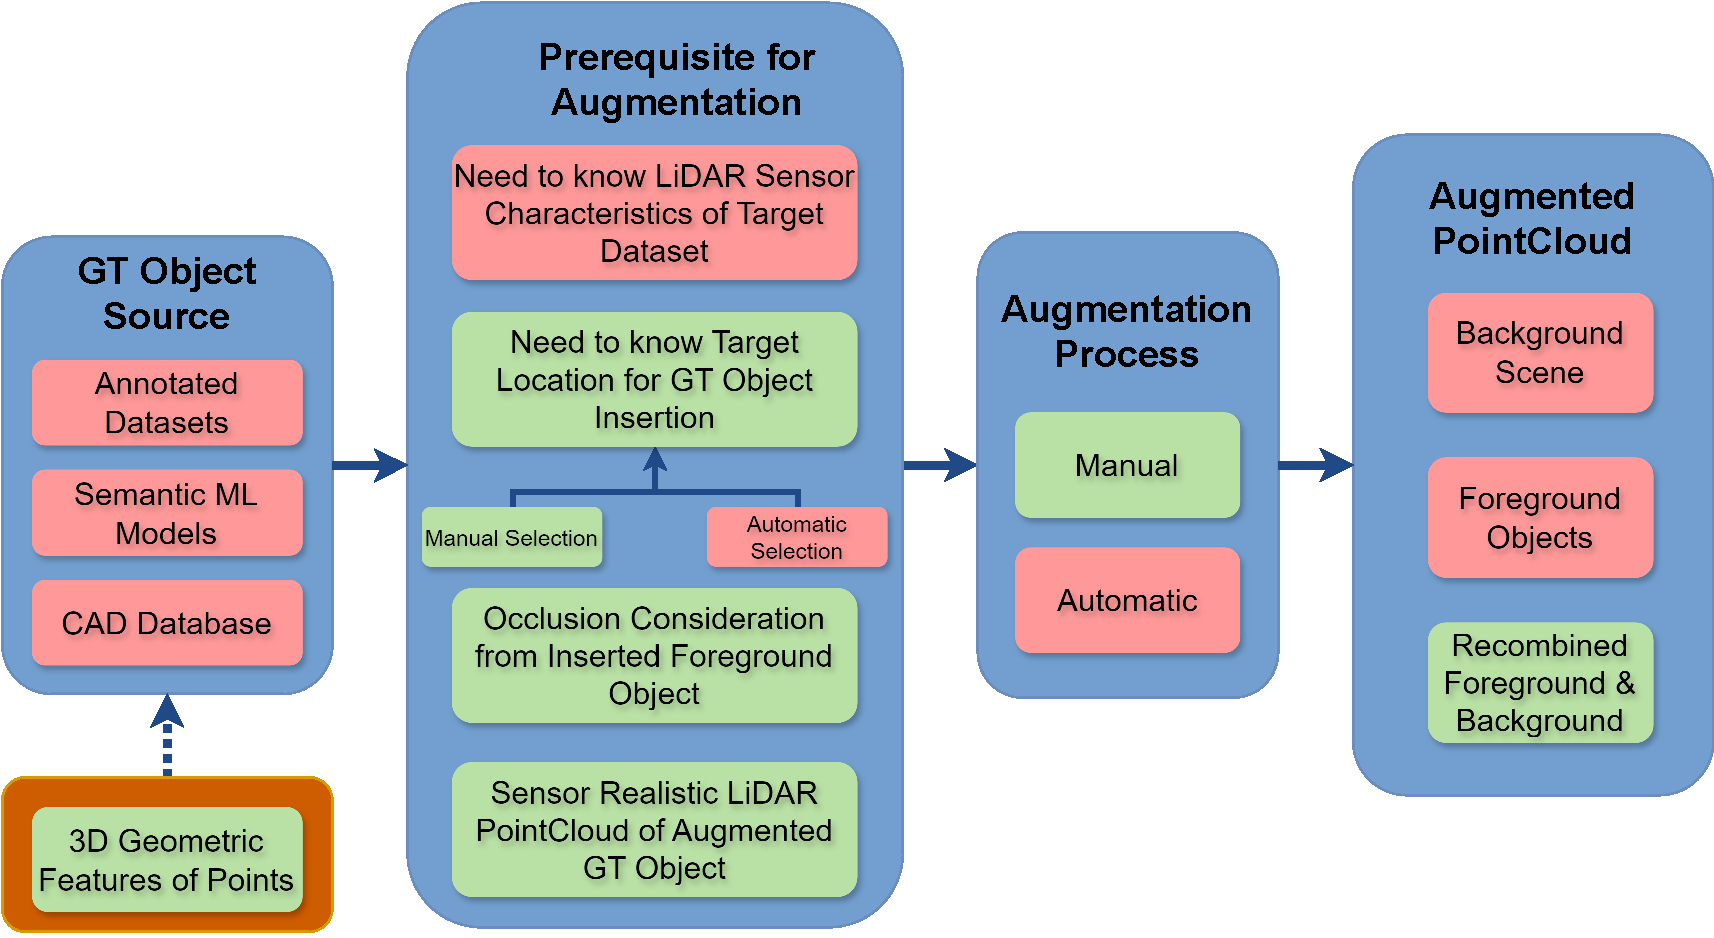
\includegraphics[width=1\linewidth]{97_graphics//related_work/related_work_block_diagram.pdf}
    \caption{Augmentation process of LiDAR Point Cloud.}
    \label{fig:sota-related_work_block_diagram}
\end{figure}


Figure \ref{fig:sota-related_work_block_diagram} illustrates current methods employed in augmenting LiDAR \acrfull{pcd}, where blue-colored blocks represent existing techniques. These methods predominantly rely on annotated datasets, Semantic ML models, or pre-existing CAD models for extracting \acrfull{gt} objects (foreground objects), as indicated by the red-colored blocks within the "GT Object Source" block. The green-colored blocks in the figure signify the approaches adopted in this thesis for scenario generation. Regardless of certain augmentation methods \parencite{9811816, dada_2023}, this thesis does not require prior knowledge of the characteristics of the LiDAR in the target dataset to be augmented. Instead, it leverages the distribution of the target point cloud in the augmentation process to accommodate these characteristics. A distinctive contribution of this work involves leveraging 3D geometric features of points within a local neighborhood for the extraction of ground truth objects from a scene, depicted by the dark orange-colored block on the far left side in figure \ref{fig:sota-related_work_block_diagram}. Implementing this method has the potential to enhance dataset diversity by injecting foreground point cloud objects into scenarios lacking foreground elements, thus addressing the class imbalance issue. Importantly, this approach eliminates the necessity for collecting and annotating new LiDAR data for scenario generation.

			\chapter{Work Environment}
\section{Work Environment}
			\chapter{Basics}

\section{LiDAR}
LiDAR refers to Light detection and ranging (Laser imaging, detection, and ranging). It can measure an object's range, angle, material reflectance, and, in certain situations, radial velocity in relation to the sensor. Numerous fields, including oceanography, meteorology, security, augmented and virtual reality, mapping, and autonomy, employ it.
\begin{figure}[htbp]
    \centering
    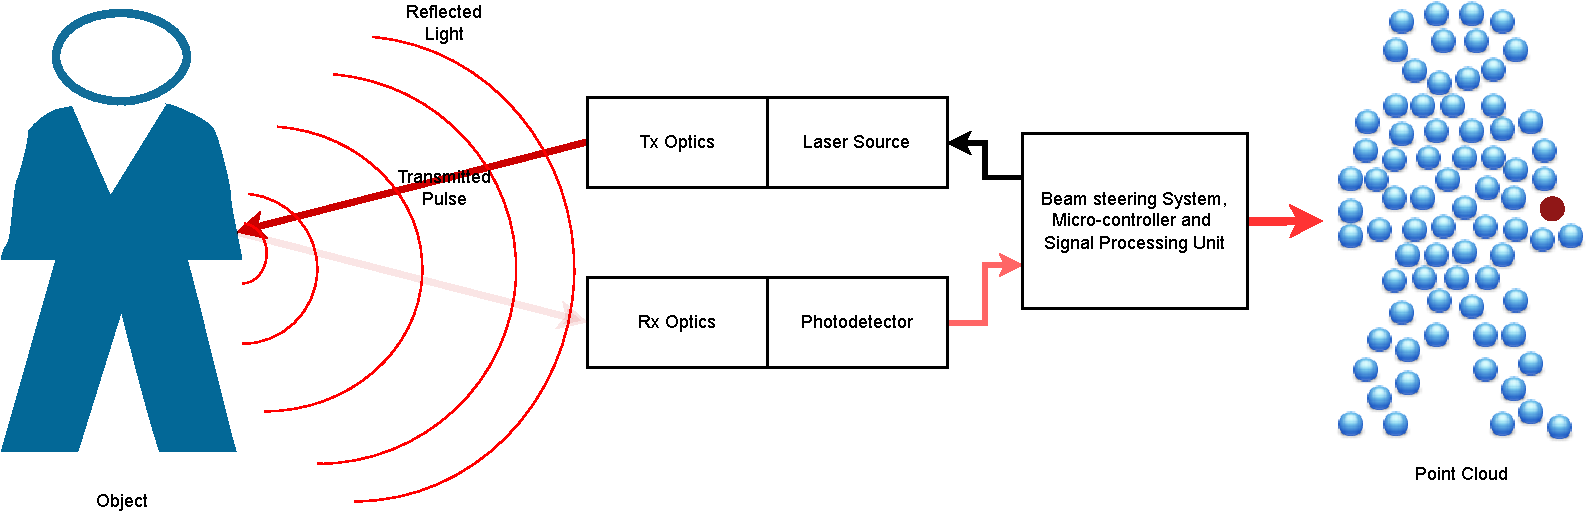
\includegraphics[width=0.8\linewidth]{97_graphics/related_work/lidar_principle.pdf}
    \caption{Operating principle of LiDAR}
    \label{fig:related_work-lidar}
\end{figure}

Laser is an electromagnetic radiation similar to that of radio frequency waves. Lasers are far shorter in wavelength than radio frequency waves, making it simple to use lenses to collimate them into narrow beams. This greatly improves LiDAR's resolution, with less than 2cm accuracy in the case of Velodyne HDL-64E LiDAR \parencite{velodyne_64}, over MIMO imaging radar and reduces the difficulty of estimating the direction of arrival. As shown in figure \ref{fig:related_work-lidar}, laser light is transmitted from the laser source, which is directed by the transmitter optics. The laser ray hits an object, reflecting the laser depending on the properties of the surface. The reflected light is captured by the photodetector system. The time of flight is calculated based on the time between the sending and receiving of the pulse. Based on the time of flight and speed of the light, the range is determined. For a round trip time \(t\), with the velocity of laser light \(c\), the distance \(d\) between the object and the laser source is determined as shown in equation \ref{eq:laser}.
\begin{equation}\label{eq:laser}
    d = \frac{c \cdot t}{2}
\end{equation}
For Speed of light(Approx.) = \(3 * 10^8 m/s^2\) and TOF = \(10 ns = 10 * 10^{-9} second\). We can use equation \ref{eq:laser} to find the distance between the laser source and the target point. Using the formula we get, the distance between the laser source and target = 0.15 meters. So it means that the distance between the laser source and the target hit point is 0.15 meters. By using the orientation of the LiDAR sensor, the exact position of the hit point is calculated. For example, if the LiDAR sensor was oriented along the x-axis, then the coordinate of the hit point would be \((x, y, z) = (0.15, 0, 0)\). Finding each point from the environment gives a point cloud representation of the environment. Data from LiDAR sensors are stored in the form of binaries. The point cloud from the LiDAR can also be represented in formats such as LAS/ LAZ, PLY, ASCII, BIN, text, etc.

\section{Testing Highly Automated Driving Systems}
Since autonomous driving systems are getting more complicated, they need to be extensively examined before being released for public use. Safeguarding the passengers' safety within an autonomous driving system presents a formidable challenge. Throughout the whole phases of development, including functional engineering and testing, integration of systems and validation, test drive and validation, etc., a comprehensive profile for testing of autonomous vehicle procedures is critically needed. Figure \ref{fig:related_work-ad_testing} shows pipelines in autonomous driving development and testing.

\begin{figure}[htbp]
    \centering
    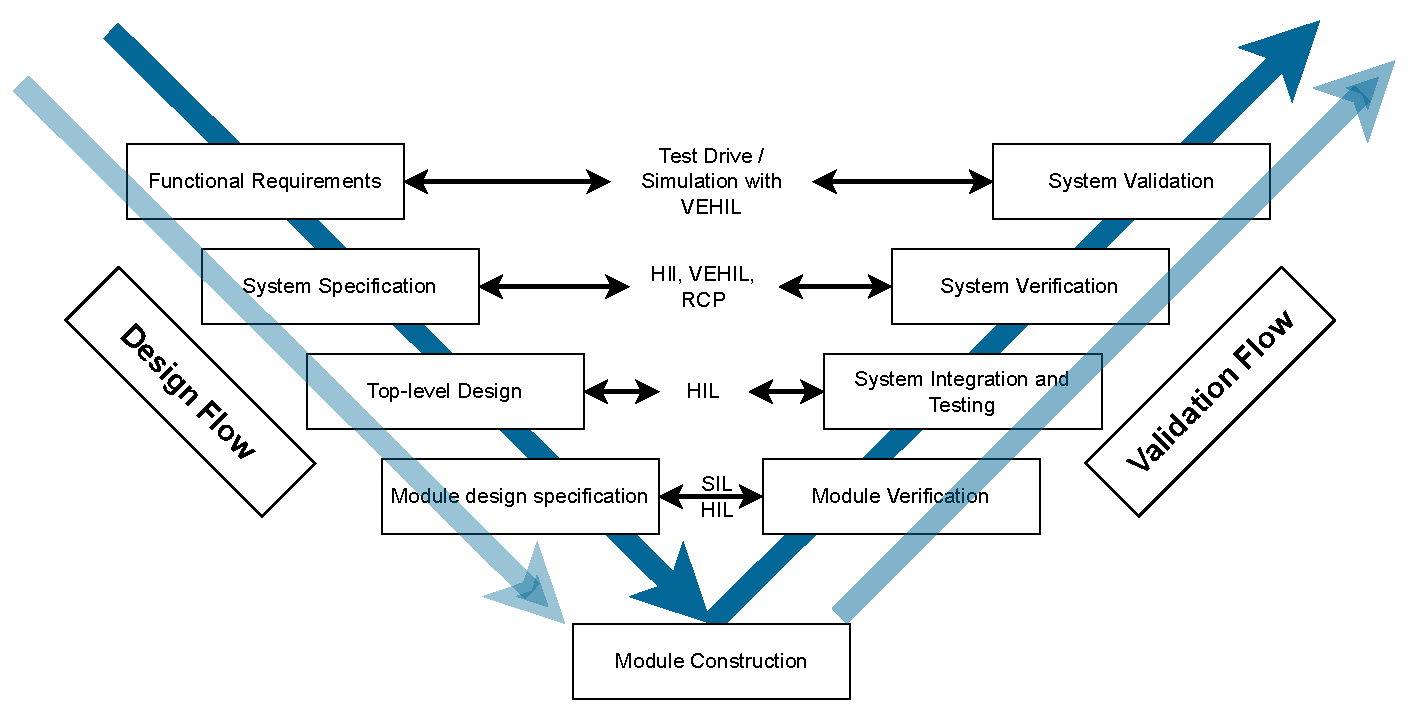
\includegraphics[width=0.7\linewidth]{97_graphics/related_work/ad_testing.pdf}
    \caption{Design and Testing pipeline for Autonomous vehicles, adapted from \parencite{ad_test_2016}}
    \label{fig:related_work-ad_testing}
\end{figure}

Various steps involve from describing functional requirements to development, validation, and verification of the requirement. \acrfull{mil}, \acrfull{sil}, \acrfull{hil}, \acrfull{vil}, or mixed simulation techniques are used to guarantee \acrshort{had} systems functionality, dependability, and safety.  

\begin{figure}[htbp]
    \centering
    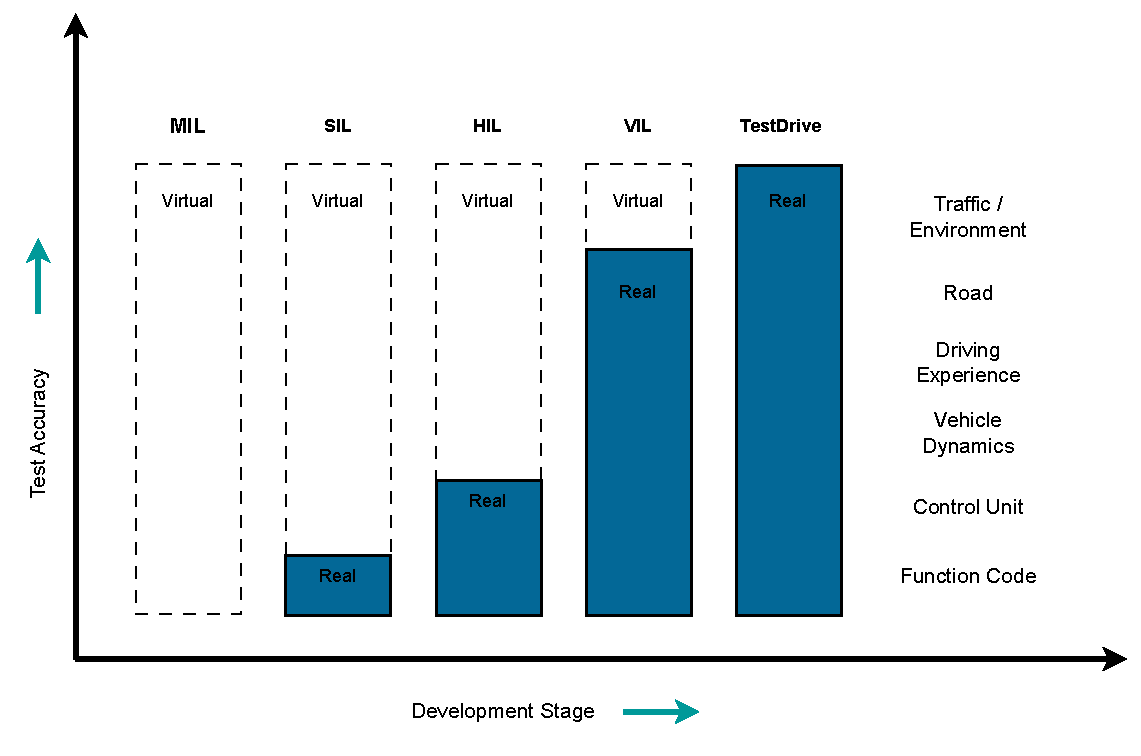
\includegraphics[width=0.7\linewidth]{97_graphics/related_work/x_in_loop_tests.pdf}
    \caption{\acrfull{xil}, adapted from \parencite{x_in_loop_test_compare}}
    \label{fig:related_work-x_in_loop_tests}
\end{figure}

A comparison of various tests concerning their reliability and development lifecycle can be viewed in figure \ref{fig:related_work-x_in_loop_tests}. \acrfull{mil} is a highly helpful tool for rapidly creating and evaluating algorithms during the prototyping or initial test stage. Pseudo code that is ready to be implemented on the \acrshort{had} system needs to be tested. Instead of testing directly on the \acrshort{had} system, which might be hazardous, the \acrfull{sil} approach is carried out. In SIL, only the pseudo-code that is to be implemented in the actual automotive controller in the HAD system is not synthetic, other domains such as \acrfull{ecu}, Vehicle Dynamics, Driving experience, road, traffic, and environment are all implemented in simulations. Numerous situations can be checked quickly because trials can be simulated more quickly than in real life. Hence, MIL and SIL are executed at the initial development phase and also have lower test accuracy in comparison to real-drive testing. Based on environmental data gathered by LiDAR, radar, stereo cameras, and other sensors, the \acrfull{ecu} controller manages the vehicle's supervisory control. With the gathered data, ECU needs to be able to understand the surrounding environment where it acts as a perception unit. It might need to be able to make decisions about safety rules, traffic laws, etc where it supports decision-making. It might also support on sending control signals to the actuators of the HAD system. An HAD system comprises multiple ECUs each focused on specific tasks, and this number only rises when pursuing towards higher level of autonomy in the HAD system. In a lab setting, \acrfull{hil} verifies the real ECU design and operational characteristics at the hardware level. Testing multiple ECUs in a synthetic environment and vehicle makes the development and verification phase of ECUs faster. \acrfull{vil} is the testing of a real vehicle in the real world but with a virtual environment. Traffic around a vehicle in the real world is simulated in VIL. It can be utilized for the evaluation of the HAD system behaviors under various critical situations without the threat of collision or hazards. Test drive comes at the final stage of the development phase. The actual vehicle is tested for the verification of the complete system. The reliability of the HAD system can be emphasized by real drive testing. During real-drive testing, an \acrfull{adas} system can get feedback from the takeover or by the engagement of the driver. This makes the process ever-learning, which improves the reliability factor of the HAD system under various scenarios.

Real-world validation of autonomous vehicles through real-drive testing is a time-consuming endeavor, as evidenced by the findings presented in \parencite{how_many_miles}, which suggest that it would take approximately 400 years of continuous driving by a fleet of 100 autonomous driving (AD) vehicles, each traveling at an average speed of 25 miles per hour, to achieve a statistically significant comparison with human driver fatality rates, with a confidence level of 95\%. However, the advent of sophisticated simulation environments developed by industry leaders has provided a promising alternative. According to a Waymo blog post \parencite{waymo_blog}, their vehicles accrue over 100 years of simulated driving experience every single day. Despite these advancements and accumulation of significant experiences, incidents such as those reported in \parencite{waymo_blog_accident} involving Waymo vehicles raise concerns about the existence of the lack of tested scenery. Domain gaps \parencite{zero_domain_gap} between real-world scenarios and those replicated in virtual environments is also a major concern. Limitations in accurately mimicking real-world landscapes and scenarios within virtual simulations may contribute to such discrepancies.


\section{SemanticKITTI Dataset}
It is an extensive dataset based on laser technology to advance semantic segmentation research in the field of autonomous driving. Comprehensive point-wise annotations are available for every sequence in the KITTI Vision Odometry Benchmark dataset \parencite{Geiger2012CVPR}. The public dataset was created by gathering real-world data to meet the rigorous requirements for functional testing and improvement of autonomous driving vehicles. The dataset contains rural roads, residential regions, freeway scenes, and inner-city traffic in Karlsruhe, Germany. For 28 classes; such as person, car, road, and vegetation; point-wise annotation is offered. This is the current state-of-the-art dataset for 3D semantic segmentation. The current SOTA 3D semantic models for autonomous driving can also be viewed at \parencite{papers-with-code}, which are also compared using the SemanticKITTI dataset. About more than 1700 hours \parencite{behley2019semantickitti} was required by a group of annotators to label and verify the labeling of the benchmark dataset. Though collected in a variety of different scenes, it does not contain all the variation of data.

\begin{figure}[htb]
    \centering
    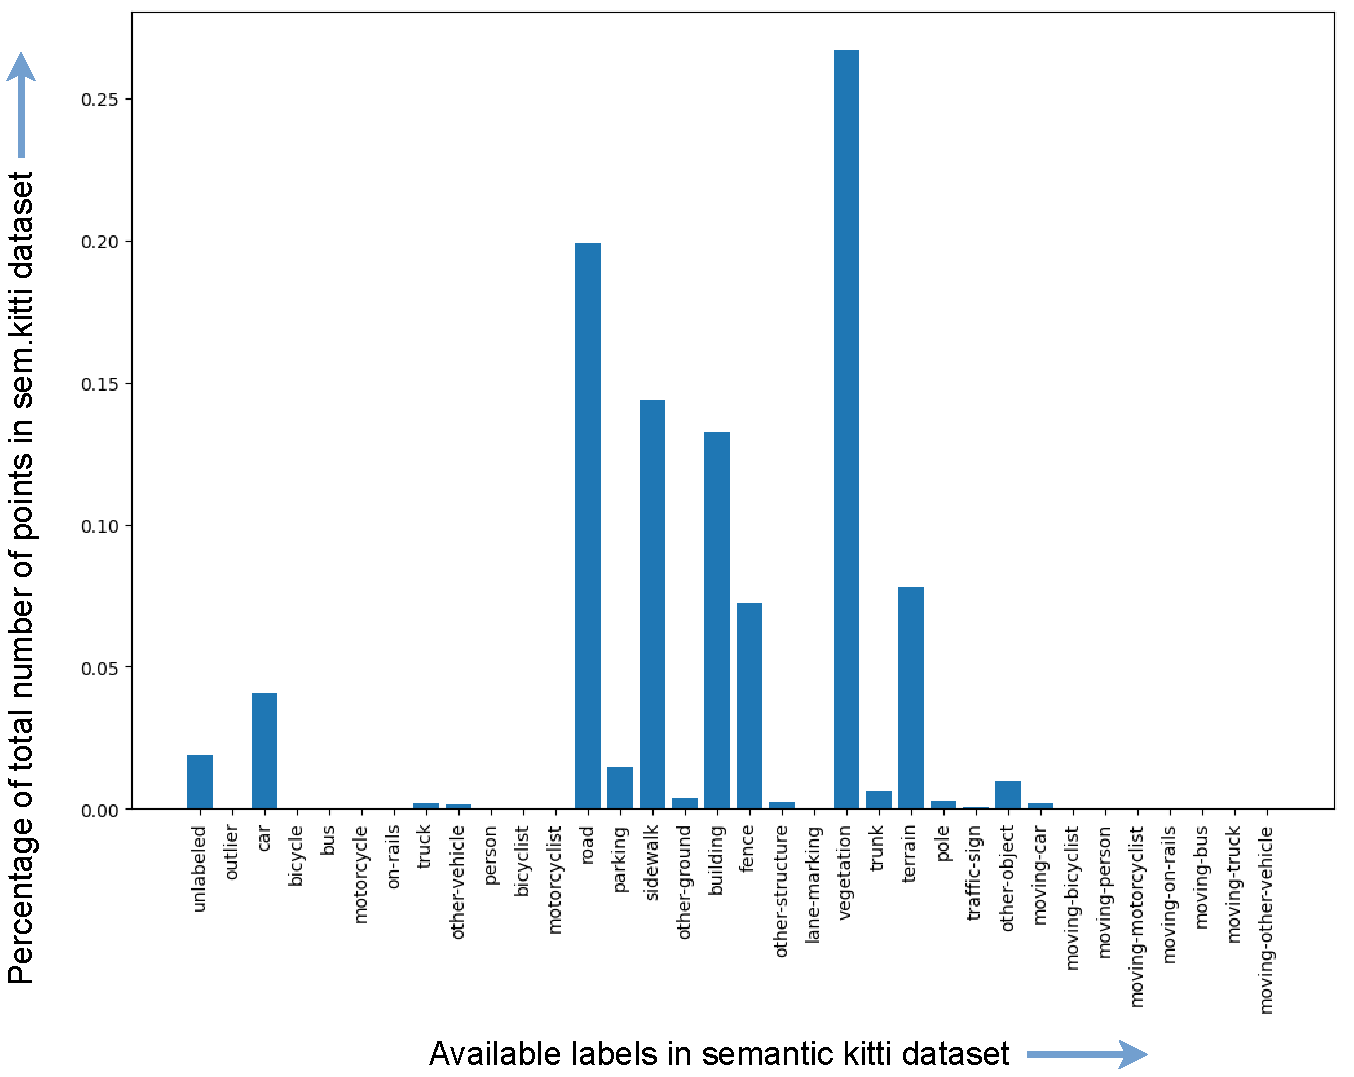
\includegraphics[width=1\linewidth]{97_graphics//related_work/ratio_with_total_points_kitti.pdf}
    \caption{Class distribution in SemanticKITTI Dataset in comparison with complete dataset points}
    \label{fig:related_work-ratio_with_total_points_kitti}
\end{figure}

Figure \ref{fig:related_work-ratio_with_total_points_kitti} shows variants of classes in comparison with total labeled classes available in the SemanticKITTI dataset \parencite{behley2019semantickitti, sem_kitti_total_points_ratio}. From the figure, it can be visualized that vegetation is the most labeled class, after that are roads, sidewalks, buildings, fences, etc. The number of labeled points for classes like person, car, trucks, etc is relatively low in comparison with classes like road, building, fence, vegetation, terrain, etc. The dataset contains scenes with either a higher density of natural scenes or scenes of downtowns, as shown in figure \ref{fig:introduction_surf_variation_in_kitti}. For a HAD system, any situation can occur when navigating in an environment such as across a river, along a mountain trail, through a desert, alongside an under-construction region, or through a huge mass of people due to demonstration, etc. Such scenarios datasets are not made available in the SemanticKITTI dataset as the data was collected in a controlled setting in Karlsruhe, Germany. This presents a gap in the dataset to represent scenarios to a maximum extent and hence only represent the real world in fragments. Also since the performance of LiDAR is also affected by environmental factors \parencite{park2023automotive}, the dataset is not enough to represent the real world to a maximum extent in the HAD context.

\begin{figure}[htb]
    \centering
    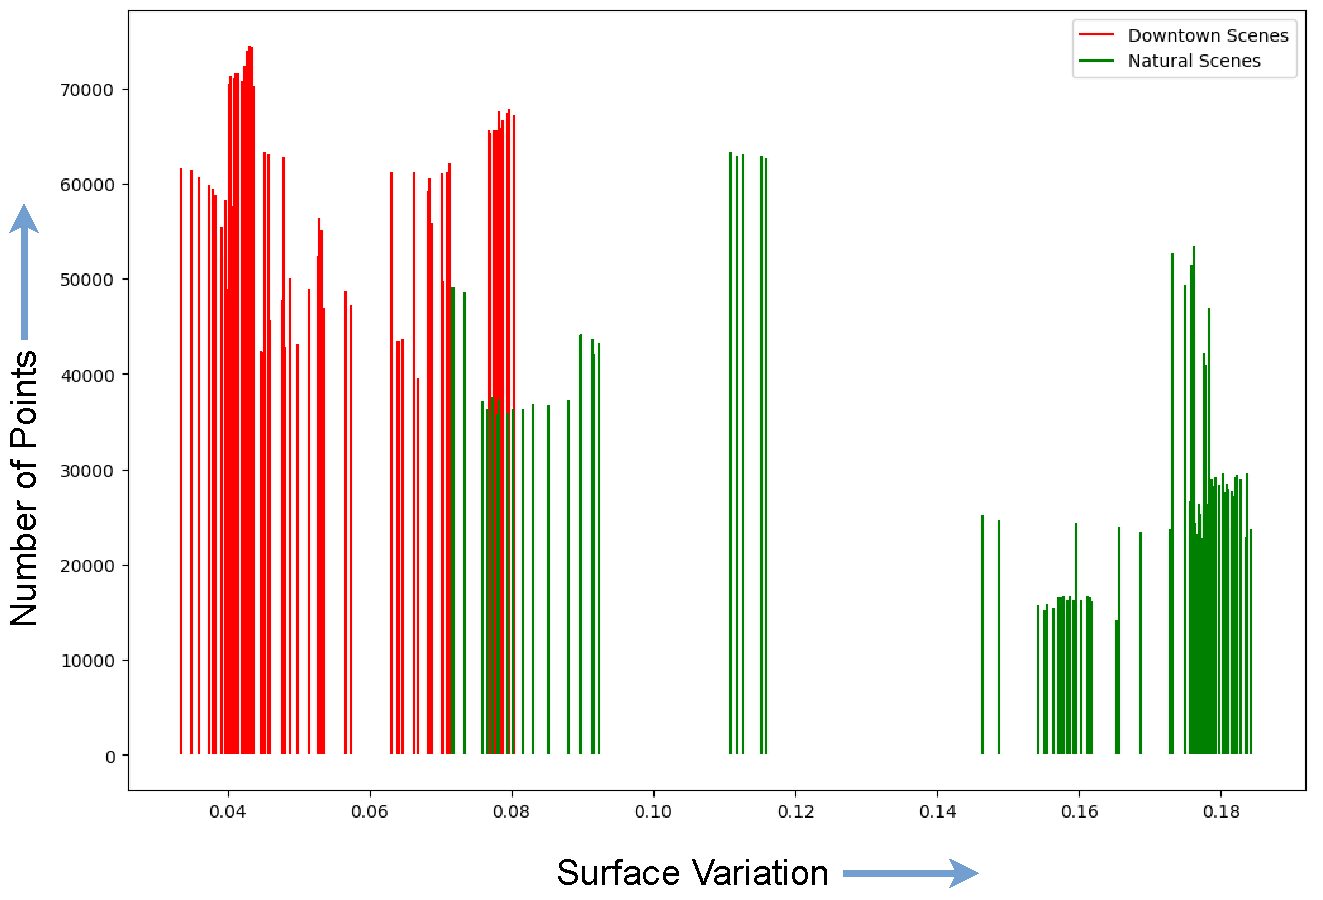
\includegraphics[width=1\linewidth]{97_graphics/related_work/downtown_and_vegetation_sv.pdf}
    \caption{Distribution of SemanticKITTI Dataset}
    \label{fig:related_work-downtown_and_vegetation_sv}
\end{figure}

From a randomly selected 100 LiDAR sequences from the SemanticKITTI dataset, point clouds for downtown scenes were calculated by accumulating points for buildings, fences, vehicles, parking, etc, unlabeled points, outliers, roads, vegetation, trunks, terrain, other-objects points were not taken to be the points for the downtown scene for the calculation in figure \ref{fig:related_work-downtown_and_vegetation_sv}. For the point clouds of natural scenes; vegetation, trunk, and terrain point clouds were combined. Point cloud aggregation is performed independently for downtown scenes and natural scenes categories within each sequence. Using hybrid search in open3d \parencite{open3d} with a sphere of radius 30 cm and maximum nearest neighbor of 6 for nearest neighbor search, surface variation was calculated using the equation \ref{eq:surf_var}. The average was taken after dividing the sum of the surface variation of each point by the total number of points for a scene for either downtown or natural scenes separately. Figure \ref{fig:related_work-downtown_and_vegetation_sv} shows the distribution of geometric features (surface variation) of the dataset for each scene. The red lines represent downtown scenes and the green lines represent natural scenes. It can be analyzed that the dataset is not evenly distributed when comparing the geometric features. The available SOTA dataset does not represent diverse scenes and it is risky, expensive, and not usually reproducible to physically test HAD vehicles on public roads. Thus, rather than doing real-world testing, simulations and other methods are opted for the initial testing phase.




\section{Simulations}
Collection of large annotated datasets like SemanticKITTI requires extensive labor work\parencite{behley2019semantickitti}. The situation becomes considerably more problematic when sparse LiDAR data is included. In order to prevent overfitting and enhance neural networks' capacity for generalization by intentionally increasing the number and variety of training data, simulations are used. Simulation are very useful in generating a variety of scenarios which is risky, costly, and rare to get from the real world. However, the variation and unpredictability of real-world situations, such as interactions between automobile drivers, pedestrians, and environmental elements, may not always be adequately captured by simulations.
A variety of simulators are currently available for testing autonomous vehicles, including CARLA, DeepDrive, Nvidia Drive Sim, Vista, VI-WorldSim, and others. \parencite{li2023choose} provides a detailed analysis of various simulators and identifies CARLA as the sole open-source, fully functional simulator that is still being maintained. As described in \parencite{li2023choose}, the examination of synthetic and real-world images within CARLA highlights the existence of disparities between simulated settings and reality. Additionally, it also discusses the shortcomings of current weather simulations, which frequently only concentrate on visual effects while not including comparable noise disturbances to sensors like LiDAR, radar, etc. There are also issues with how accurately car dynamics are simulated; numerous physics models only behave reliably when the parameters of steering angle, acceleration, and velocity stay low \parencite{7225830}.

\begin{figure}[htbp]
    \centering
    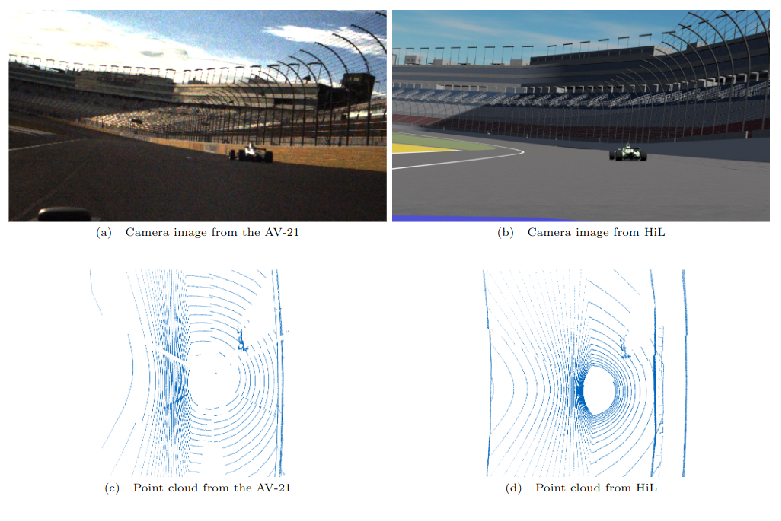
\includegraphics[width=0.8\linewidth]{97_graphics/related_work/real_vs_simulation_difference.pdf}
    \caption{Real world vs Simulation difference \parencite{sauerbeck_learn_Year}}
    \label{fig:related_work-real_vs_simulation}
\end{figure}

Data captured on a series of Indy Autonomous Challenge 2021 \parencite{sauerbeck_learn_Year} shows the difference between the real environment and synthetic simulation. The assumptions that underpin virtual sensor models do not always stand valid in practical situations. Content and Appearance gap between the synthetic and real-world is also discussed in \parencite{care_real_and_syn_gap}. For high accuracy, we need simulation with a low domain gap concerning the real world. It is difficult to model HAD simulators involving LiDAR because of the following reasons \parencite{zero_domain_gap}. 
\begin{itemize}
    \item Unreturned pulses because of pulse's power decay.
    \item Multiple echoes from the environment resulting in multiple peaks in the returning signal.
    \item Spurious returns due to volume scattering, blooming, beam divergence, multi-echo, etc.
    \item Noisy points because of randomness in the real world, retro-reflectors.
    \item Rolling shutter and motion blur in moving vehicle.
\end{itemize}

\section{Scenario-Based Testing}
According to \parencite{def_scene}, a scene is a description of a particular moment in time of the environment that includes the scenery, dynamic aspects, self-representations of all the performers and spectators, and the interactions between those entities. A scenario explains how various scenes in a series of sequences of scenes evolve over time. Three distinct scenarios are defined according to \parencite{menzel2018scenarios}. They are functional scenarios, logical scenarios, and concrete scenarios. 

\begin{figure}[htbp]
    \centering
    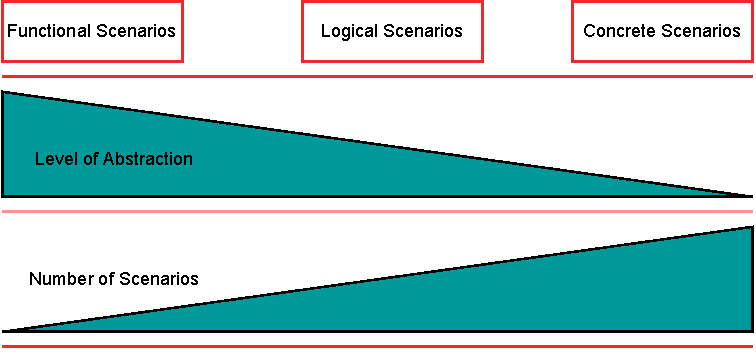
\includegraphics[width=0.75\linewidth]{97_graphics/related_work/three_different_scenarios.pdf}
    \caption{Three different scenarios, adapted from \parencite{menzel2018scenarios}}
    \label{fig:related_work-3scenarios}
\end{figure}

As shown in figure \ref{fig:related_work-3scenarios}, the level of abstraction decreases with an increase in several scenarios from functional to concrete scenarios. Functional scenarios come in the concept phase where the scenarios can be described by human experts in the natural language. A logical scenario appears in the system development phase where the scenario is explained with various parameter ranges. Concrete scenarios are represented for the test phase where the concrete state values are defined to guarantee scene replicability and facilitate testing techniques. For describing the parameters of the logical and concrete scenario, a five-layer model is explained in \parencite{bagschik2018ontology}, as shown in figure \ref{fig:related_work-5layer_model}.

\begin{figure}[htbp]
    \centering
    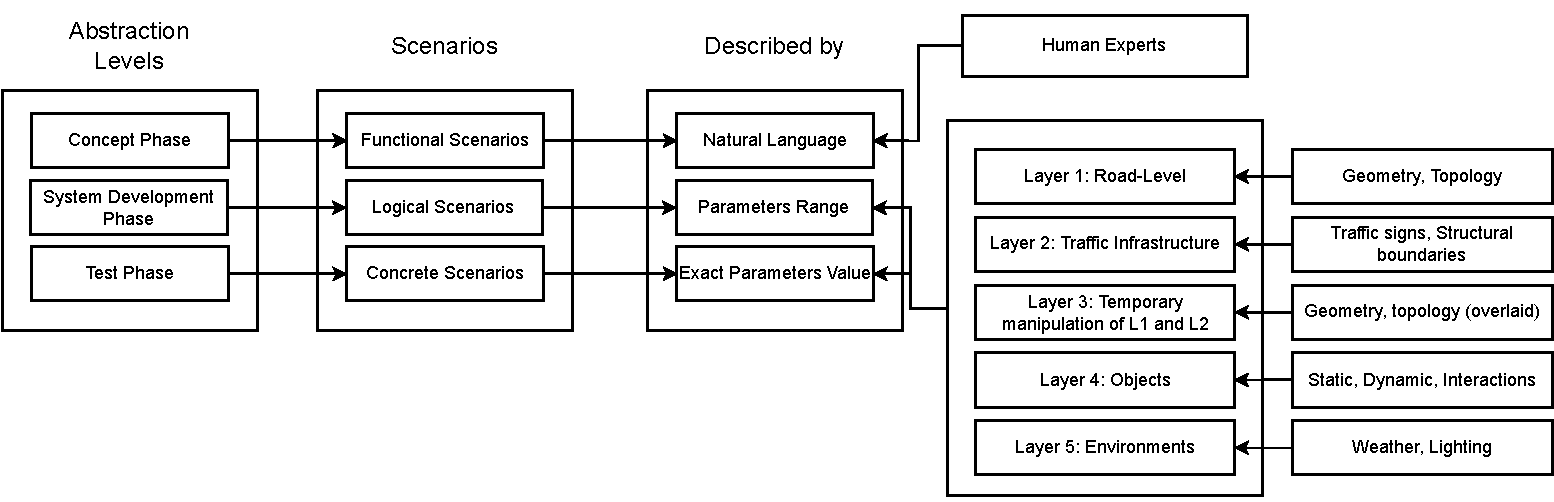
\includegraphics[width=1\linewidth]{97_graphics/related_work/scenario_based_testing.pdf}
    \caption{Abstraction levels, scenarios, and explanation terms. Adapted from \parencite{bagschik2018ontology} and \parencite{menzel2018scenarios}
    }
    \label{fig:related_work-5layer_model}
\end{figure}

To arrange all the data in a database of knowledge to represent scenes, a model with multiple layers is explained as illustrated in the figure \ref{fig:related_work-5layer_model}. The topology and markings of the road are described in the first layer. The model's hierarchical ideas describe how to construct legitimate road fragments for traffic scenes by assembling geometries that represent lanes. Road-level traffic infrastructure is added in the second layer. Not every stationary object, such as vegetation, is a part of the infrastructure for traffic. Classes that reflect the marking, routing, and security requirements for building sites are included in the third layer. In the ensuing traffic scenarios, the modifications made to the original layout are identified as manipulation. The fourth layer models every object that may not be included in the transportation infrastructure. It is possible to arrange both stationary and mobile objects without significantly altering the connections within the traffic infrastructure. Participants in traffic are divided into object classes, such as vehicles, trucks, bicycles, etc. Environmental conditions like weather and lightning are considered on the fifth layer. Additionally, the impact on the interactions amongst traffic participants is taken into account, leading to varying parameter ranges for relative parameters.

With the help of the scenarios database and knowledge, new scenarios are generated. The information content and level of abstraction in each generated or extracted scenario categorize the scenario types within the \acrfull{odd}. The scenarios database is created with expert knowledge or by varying the parameter range and values. As described on \parencite{bagschik2018ontology}, concrete scenarios are selected based on a testing-based approach or falsification-based approach. In the testing-based approach, range sampling and distribution sampling are done from a logical scenario database, and concrete scenarios are extracted. Based on macroscopic and microscopic assessment, a scenario is selected. A substantial quantity of data needs to be made available to make a macroscopic (statistical) assessment regarding the overall effect of autonomous vehicles on traffic. Specific traffic scenarios are put to the test and assessed. Microscopic evaluation is the assessment of a single scenario. The purpose of the falsification techniques is to locate counterexamples that break safety regulations while doing microscopic evaluations. Based on criticality, complexity, etc concrete scenarios are selected from the scenario database which undergoes microscopic assessment. Scenarios could be samples from the accident database or by changing the criticality of available concrete scenarios. Increasing the scenario's complexity can likewise raise the likelihood of discovering a counterexample.
The chosen specific scenarios can be executed in a variety of testing environments. These can be carried out using \acrfull{xil} simulation \parencite{x_in_loop}, which offers a higher level of virtualization, or in the actual world through field or proving-ground experiments. Since XIL offers numerous benefits in terms of, for example, expenses, risks, and safety, nearly all references employ simulation as part of their proof of concept.
Scenario-based testing involves organizing circumstances relevant to the testing system in a systematic manner. Implementing a derived logical scenario necessitates keeping irrelevant circumstances constant for a specific test argumentation while adjusting relevant ones through the execution of concrete scenarios. Achieving this demands positioning prototypes such as persons within the scene in a controlled manner, which is impractical in reality and feasible in simulation, though without valid sensor data.

\section{Enhancing Methods for Testing LiDAR-based Functions}
Enhancing LiDAR-based functions involves improving the capabilities and performance of LiDAR systems for various applications. The different methods used to improve the LiDAR-based functions are described in below points :
\begin{itemize}
    \item \textbf{LiDAR Data Augmentation : }
    Capturing data representing diversities of scenes in the real world is expensive and laborious. Simulations are also utilized in addition but because of the domain gap between the real and synthetic world, the captured data do not accurately represent the real world environment. LiDAR data augmentation could be approached where data within the LiDAR is changed like scaled, transformed, rotated, etc. Combining synthetic data of objects with real-world point clouds is also an option.
    \item \textbf{Sensor Data Fusion : }
    The system's reliability is increased by integrating LiDAR data with information from other sensors, including cameras, radar, and \acrshort{gps}, which also improves perception accuracy and redundancy. Data from the camera sensor can be mapped to the LiDAR point cloud to make use of a robust image segmentation model for the localization of objects in the point cloud. \parencite{pointpainting2019} make use of segmentation information obtained from the image detection algorithm to "paint" the points of a 3D point cloud. In the context of integrating data from various sensors, challenges such as ensuring the synchronization of data streams must be addressed.
    \item \textbf{Security testing and Attack Simulations : }
    Testing LiDAR systems for possible security risks like jamming or spoofing guarantees their robustness and resilience when used in real-world scenarios.  Adversarial scenario simulation is used to evaluate LiDAR performance under several attack vectors, which aids in finding weaknesses and strengthening system defenses.
    \item \textbf{Resolution Enhancement and Noise Reduction : }
    Post-processing techniques like interpolation or the use of multi-beam LiDAR may be approached to enhance the resolution of LiDAR data. Accurate object detection and mapping can be improved by using point clouds with higher resolutions, which capture finer aspects of the scene. Different techniques can be employed to remove noise from LiDAR point clouds to make the data more accurate and clear. Strategies like Gaussian filtering and statistical outlier elimination can assist in lowering noise brought on by flaws in the sensor or environmental influences.
    \item \textbf{Use of Contextual Information : }
    Using additional environmental cues to enhance the comprehension of the 3D point clouds is an effective way to employ contextual information in LiDAR data analysis. LiDAR-based algorithms can achieve better scene understanding and object recognition by adding contextual information such as spatial interconnections, object interactions, and scene interpretation. Contextual indications, such as building structures, traffic signs, and road markings, can be particularly helpful in determining the presence and placement of things like cars, pedestrians, and other obstacles. Contextual data also makes LiDAR systems more resilient and reliable in real-world applications like autonomous driving, urban planning, and environmental monitoring by allowing them to adjust dynamically to changing environmental conditions. Local neighborhood features of points play a vital role in understanding the context.
\end{itemize}


\section{Statistical Computation of LiDAR Point Cloud Descriptors}
\subsection{Mathematical Operations in 3D Space}
\subsubsection{Scalars and Vectors}
A scalar is a quantity that has only magnitude or size without any associated direction. Scalars are often employed to quantify quantities like mass, temperature, energy, speed, or time since they are represented by a single real integer. A quantity having both magnitude and direction is called a vector. An ordered collection of real numbers, or components, and a direction in space are used to represent vectors. Vectors are commonly depicted in 3D space as arrows that point from the origin to a designated location in the space.


\begin{figure}[htbp]
    \centering
    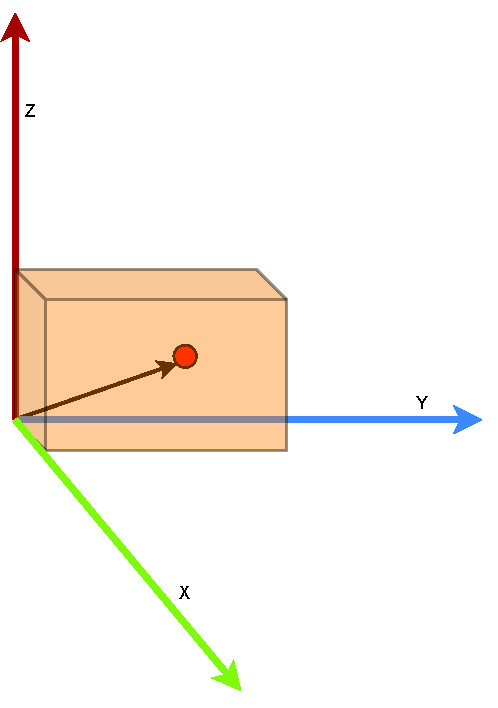
\includegraphics[width=0.4\linewidth]{97_graphics/related_work/scalar_and_vector.pdf}
    \caption{A 3D Cube in XYZ Coordinate System.}
    \label{fig:related_work-scalar_and_vector}
\end{figure}

In the figure \ref{fig:related_work-scalar_and_vector}, the volume of the cuboid represents the scalar quantity, and the black arrow pointing to a red point in the cuboid represents a vector. Scalars can be added, subtracted, multiplied, or divided just like ordinary numbers. Various mathematical operations can be performed on vectors like scalar multiplication, vector addition, dot product, cross product, etc. Equation \ref{eq:dot_product}, \ref{eq:cosine_angle}, \ref{eq:cross_product}, \ref{eq:sine_angle}, \ref{eq:angle_between_vectors} gives a general idea of calculating the angle between two vectors using the vector operations.
\begin{itemize}
    \item \textbf{Dot Product}:
    \begin{equation}\label{eq:dot_product}
        \mathbf{p} \cdot \mathbf{q} = p_x \cdot q_x + p_y \cdot q_y + p_z \cdot q_z
    \end{equation}
    \item \textbf{Cosine of Angle between two vectors}:
    \begin{equation}\label{eq:cosine_angle}
        \cos\theta = \left(\frac{\mathbf{p} \cdot \mathbf{q}}{|\mathbf{p}| \cdot |\mathbf{q}|}\right)
    \end{equation}
    \item \textbf{Cross Product}:
    \begin{equation}\label{eq:cross_product}
        \mathbf{p} \times \mathbf{q} = (p_y q_z - p_z q_y, p_z q_x - p_x q_z, p_x q_y - p_y q_x)
    \end{equation}
    \item \textbf{Sine of Angle between two vectors}:
    \begin{equation}\label{eq:sine_angle}
        \sin\theta = \left(\frac{|\mathbf{p} \times \mathbf{q}|}{|\mathbf{p}| \cdot |\mathbf{q}|}\right)
    \end{equation}
    \item \textbf{Angle between two vectors}:
    \begin{equation}\label{eq:angle_between_vectors}
        \theta = \arctan\left(\frac{\sin(\theta)}{\cos(\theta)}\right)
    \end{equation}
\end{itemize}

\subsubsection{Translation, Rotation, and Transformation}
Moving an object from one place to another in three dimensions without modifying its shape or orientation is referred to as translation. It entails moving every point on the item in a certain direction by a predetermined amount. In three-dimensional space, rotation is the process of shifting an object's orientation around a designated axis or point. It involves rotating the object by a certain angle about the selected axis or point. A combination of translation, rotation, scaling, and other operations performed on an object is referred to as transformation in 3D space. It enables one-step changes to the object's size, location, and orientation. The operations are represented by the equation \ref{eq:translation}, \ref{eq:rotation}, \ref{eq:transformation}. Where (x,y,z) represents a point in cylindrical coordinates and T represents any transformation matrix.

\begin{itemize}
    \item \textbf{Translation}:
    \begin{equation}\label{eq:translation}
        \begin{pmatrix}
        x' \\
        y' \\
        z'
        \end{pmatrix}
        =
        \begin{pmatrix}
        x + a \\
        y + b \\
        z + c
        \end{pmatrix}
    \end{equation}
    
    \item \textbf{Rotation}:
    \begin{equation}\label{eq:rotation}
        \begin{pmatrix}
        x' \\
        y' \\
        z'
        \end{pmatrix}
        =
        \begin{bmatrix}
        \cos(\theta) & -\sin(\theta) & 0 \\
        \sin(\theta) & \cos(\theta) & 0 \\
        0 & 0 & 1
        \end{bmatrix}
        \begin{pmatrix}
        x \\
        y \\
        z
        \end{pmatrix}
    \end{equation}
    
    \item \textbf{Transformation}:
    \begin{equation}\label{eq:transformation}
        \begin{pmatrix}
        x' \\
        y' \\
        z'
        \end{pmatrix}
        =
        T
        \begin{pmatrix}
        x \\
        y \\
        z
        \end{pmatrix}
    \end{equation}
\end{itemize}

\subsection{Nearest Neighbour Search}
A basic issue in mathematics and computer science, especially in the areas of computational geometry and data structures, is nearest neighbor search. A collection of points P serves as the problem's input. The objective is to locate the point in the set P that is closest to a given query point, q. This necessitates O(n) comparisons naively since we must compare q to every point in P. Using the brute-force technique is not computationally possible when the number of points is very huge. As a result, our objective is to pre-process the input and produce a data structure that can respond to queries rapidly. Distance metric, such as the Minkowski, Manhattan, or Euclidean distances, is usually utilized to determine the separation between two positions, which can be used to create new data structures for effective search. The Euclidean distance, which is the square root of the total squared differences in each coordinate, is frequently used in the context of three-dimensional space. Nearest Neighbor has countless applications and is used in numerous computer science fields, including computational linguistics, machine learning, and image recognition. It's crucial to remember that, despite all recent developments in the field, exhaustive search remains the only technique that can reliably retrieve the precise nearest neighbor. Because of the "curse of dimensionality", finding the exact nearest neighbor is impractical when the dimensionality of the data is large and so an Approximate Nearest Neighbor was introduced. Techniques like Vector Transformation, Vector Encoding, None Exhaustive Search Components were introduced to preprocess the data into an efficient index. Numerous space-partitioning techniques have been created to address the nearest neighbor search issue. The k-d tree (a binary tree), which repeatedly splits the search space into two areas with half of the points of the parent region, is arguably the most straightforward. By analyzing the query point at each split, queries are executed by traversing the tree from the root to a leaf. It might also be necessary to assess nearby branches that could contain hits, depending on the query's distance specification. Parameters, such as radius and maximum number of nearest neighbors, could be adjusted for a search of the nearest neighbor of a query point.
\begin{figure}[htbp]
    \centering
    \begin{minipage}[b]{0.45\textwidth}
    \centering
    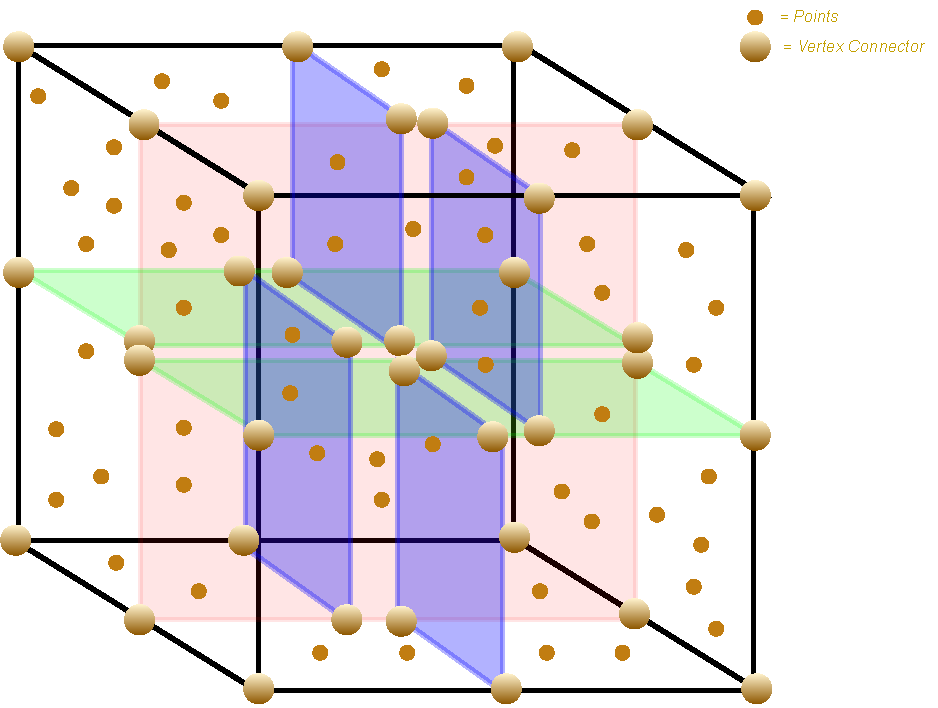
\includegraphics[width=1\linewidth]{97_graphics/related_work/kdtree_cube.pdf}
    \caption{3D Space containing Points with dividing Hyperplanes.}
    \label{fig:related_work-kdtree}
    \end{minipage}
    \hfill
    \begin{minipage}[b]{0.45\textwidth}
    \centering
    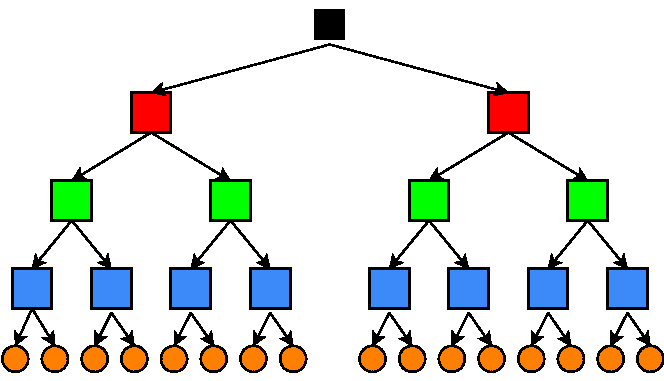
\includegraphics[width=1\linewidth]{97_graphics/related_work/kdtree_tree.pdf}
    \caption{Tree structure showing leaf nodes, root nodes.}
    \label{fig:related_work-search_tree}
    \end{minipage}
\end{figure}

In figure \ref{fig:related_work-kdtree}, the initial partition (the red vertical plane) divides the root cell into two subcells. The subsequent division (the green horizontal planes) further divides each of those subcells into two subcells, and so on. The splitting plane in the three-dimensional space represents the non-leaf node. All non-leaf nodes can be viewed as inherently creating a dividing hyperplane, or half-space, that divides the available region into two halves. Points to the left of the hyperplane are represented by the subtree on the left side of that node, while points to the right of the hyperplane are represented by the subtree on the right side. Here's how to figure out the orientation of the hyperplane: each node in the tree corresponds to one of the k dimensions, and the hyperplane is oriented perpendicularly to the axis of that dimension. This splitting of 3D dimension into cells can be discussed with the figure \ref{fig:related_work-search_tree}. The square boxes in the figure represent non-leaf nodes. The circular shapes in orange color represent the points in the 3D space. A 3D space is split into two halves by a red plane in figure \ref{fig:related_work-kdtree}. This is represented by the black root node separated into two red-colored child nodes - left and right node. The red plane is further divided into two green planes in the 3D space, which is represented by two green-colored child nodes of red parent nodes. The space separated by green planes is further divided by blue planes, which contain the points. A search of the nearest neighbor is done by traversing the tree from the root to the leaf nodes, where each comparison is done for each dimension of k-dimensions alternatively when traversing the parent nodes.

\subsection{Variance, Covariance, and Covariance Matrix}
The dispersion or spread of a single random variable is measured by variance. The variance of X in 3D space expresses the degree to which the values of X differ from their mean value. The amount that two random variables fluctuate together is measured by covariance. 

\begin{itemize}
    \item \textbf{Variance of variable X:}
    \begin{equation}
    \text{Var}(X) = \frac{1}{n} \sum_{i=1}^{n} (X_i - \bar{X})^2
    \end{equation}
    
    \item \textbf{Covariance between X and Y:}
    \begin{equation}\label{eq:covariance}
    \text{Cov}(X, Y) = \frac{1}{n} \sum_{i=1}^{n} (X_i - \bar{X})(Y_i - \bar{Y})
    \end{equation}
    
    \item \textbf{Covariance Matrix in 3D Spaces:}
    The covariance matrix \(C\) is given by:
    \begin{equation}\label{eq:covariance_matrix}
    C = \begin{bmatrix}
    \text{Var}(X) & \text{Cov}(X, Y) & \text{Cov}(X, Z) \\
    \text{Cov}(Y, X) & \text{Var}(Y) & \text{Cov}(Y, Z) \\
    \text{Cov}(Z, X) & \text{Cov}(Z, Y) & \text{Var}(Z)
    \end{bmatrix}
    \end{equation}
\end{itemize}

The equation \ref{eq:covariance_matrix} is very useful in giving us insights about the dataset of variables by helping us to understand the relation between variables, in our case in 3D space. It can be summarized in below points :
\begin{itemize}
    \item  Negative covariances show that variables move in the opposite way.
    \item Positive covariances show that variables tend to rise or decrease together.
\end{itemize}

It can be utilized to construct a transformation matrix known as a whitening transformation, which, from another angle, enables one to evaluate the best foundation for compactly describing the data or, alternatively, to fully decorrelate the data. Therefore, the covariance matrix can be viewed as a linear transformation that maps vectors from one d-dimensional space to another d-dimensional space. Dimensionality Reduction, financial portfolio optimizations, clustering, statistical inference, and calculation of surface orientations are some use cases from the use of covariance matrix.

\subsection{Eigen Values and Eigen Vectors}
 The vectors that a linear transformation works on are rotated, stretched, or sheared. The vectors that are merely stretched; they do not rotate or shear; are known as its eigenvectors. The associated eigenvalue for an eigenvector is the value that influences an eigenvector to change in length or direction. If the eigenvalue is negative, the eigenvector's direction is transformed. Non-zero vectors that, upon application of a linear transformation (expressed by a matrix), are scaled by the associated eigenvalues are Eigenvectors. Eigenvectors depict the directions that a transformation acts in, just extending or compressing; they do not alter the direction. For a transformation matrix "T", the corresponding eigen values and eigen vectors are represented by equation \ref{eq:eigen}. If \( \lambda_1, \lambda_2, \) and \( \lambda_3 \) represents the eigen values of a 3D covariance matrix then a relation can be showed by equation \ref{eq:eigen_relation}.

\begin{itemize}
    \item Eigenvalue (\( \lambda \)) and Eigenvector (\( \mathbf{v}^{\rightarrow} \)):
    \begin{equation}\label{eq:eigen}
    \text T \mathbf{v}^{\rightarrow} = \lambda \mathbf{v}^{\rightarrow}
    \end{equation}
    \item Relation between eigen values for a 3D Covaraiance matrix :
    \begin{equation}\label{eq:eigen_relation}
    \lambda_1 \geq \lambda_2 \geq \lambda_3 \geq 0
    \end{equation}
    
\end{itemize}

By undergoing the process of eigen decomposition using the equation \ref{eq:eigen}, eigen vectors and eigen values can be calculated from the covariance matrix. Principal components analysis makes use of eigenvectors and eigenvalues, where eigenvectors are associated with the principal components, and eigenvalues explain the discrepancies of the principal components. Some Key features can be described as :
\begin{itemize}
    \item High value of eigenvector captures directions of maximum variance of data.
    \item Low value of eigenvector captures directions of minimum variance of data.
    \item Sum of eigenvalues gives the total variation of points from the center of gravity.
    \item For n-dimensional data, at most n eigenvalues and corresponding eigenvectors is possible.
\end{itemize}

Selecting a subset of the eigenvectors that represent the maximum variance of data allows for dimensionality reduction while preserving the most important features. It is used in applications like normal calculation, feature extraction, vibration analysis, etc.

\subsection{Normal Estimation}
In computer vision, computer graphics, and geometric modeling, normal estimation is an essential procedure. To accurately recreate the underlying surface geometry, surface reconstruction techniques frequently begin with normal estimation, which involves determining the normals of a point cloud or a group of surface points. When working with scarce or noisy data, normal information helps create surfaces that are accurate and smooth. Normals aid in the identification of sharp edges, the determination of surface features, and the direction of different mesh processing activities. Rendering scenes with accurate normal estimates makes them look more realistic. For robots to navigate challenging environments and interact with items effectively, accurate normal information is necessary.

\begin{figure}[htbp]
    \centering
    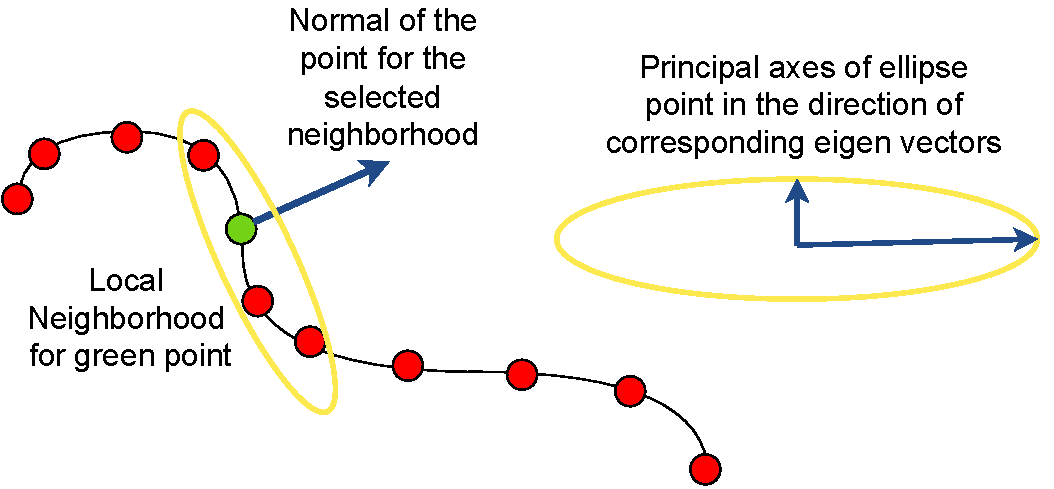
\includegraphics[width=0.5\linewidth]{97_graphics//related_work/normal_estimation.pdf}
    \caption{Surface represented by points and selection of local neighborhood, adapted from \parencite{normal_estimation}}
    \label{fig:related_work-normal_estimation}
\end{figure}

In figure \ref{fig:related_work-normal_estimation}, the black curve represents a surface represented by a group of red points. The orientation of the surface in the region bounded by the yellow color curve represents the normal of the surface for the yellow-bounded region, this is represented by the direction of the blue arrow. We can find the normal of the surface at a point by the following steps \parencite{normal_estimation} referencing the figure \ref{fig:related_work-normal_estimation} :

\begin{enumerate}
    \item Identify the neighbors for the point (represented by a green-colored point in the figure) through which the normal is to be calculated. The neighborhood is represented by the yellow ellipse. 
    \item Calculation of Covariance Matrix from the local neighborhood.
    \item Calculation of Eigen Values and Eigen Matrix by Eigen decomposition of Covariance Matrix.
    \item The Direction of the eigenvector corresponding to the least eigenvalue is the surface normal. (i.e. direction of least variance of the features)
\end{enumerate}

\subsection{Statistical Point Cloud Measurement}
The spatial placement of individual 3D points implicitly represents important geometric information found in 3D point clouds. These attributes should be calculated with particular spatial support because context is not taken into account when considering individual points \parencite{weinmann2013feature}. Usually, the local neighborhood surrounding each 3D point is retrieved in order to explain this implicit information sufficiently. For example, defining a fixed size sphere around a point in a point cloud could give a local neighborhood where all the points lying in the sphere are the neighbors \parencite{lee2002perceptual}. The local 3D structure can be described directly by the eigenvalues of a 3D covariance matrix which follows the equation \ref{eq:eigen}. Alternatively, additional measures that capture unique geometric features can be deduced based on these eigenvalues. Utilizing the relation of eigenvalues from equation \ref{eq:eigen_relation}, the definition of various features is referenced from \parencite{weinmann2013feature}.

\begin{itemize}
    \item Linearity (\( L_{\lambda} \)):
    \begin{equation}
        L_{\lambda} = \frac{\lambda_1 - \lambda_2}{\lambda_1}
    \end{equation}
    
    \item Planarity (\( P_{\lambda} \)):
    \begin{equation}
        P_{\lambda} = \frac{\lambda_2 - \lambda_3}{\lambda_1}
    \end{equation}
    
    \item Scatter or Sphericity (\( S_{\lambda} \)):
    \begin{equation}
        S_{\lambda} = \frac{\lambda_3}{\lambda_1}
    \end{equation}
    
    \item Omnivariance (\( O_{\lambda} \)):
    \begin{equation}
        O_{\lambda} = \left( \lambda_1 \cdot \lambda_2 \cdot \lambda_3 \right)^{\frac{1}{3}}
    \end{equation}
    
    \item Anisotropy (\( A_{\lambda} \)):
    \begin{equation}
        A_{\lambda} = \frac{\lambda_1 - \lambda_3}{\lambda_1}
    \end{equation}
    
    \item Surface Variation \parencite{rusu2009semantic} (\( C_{\lambda} \)):
    \begin{equation}\label{eq:surf_var}
        C_{\lambda} = \frac{\lambda_3}{\lambda_1 + \lambda_2 + \lambda_3}
    \end{equation}
    
\end{itemize}

\begin{figure}[htbp]
    \centering
    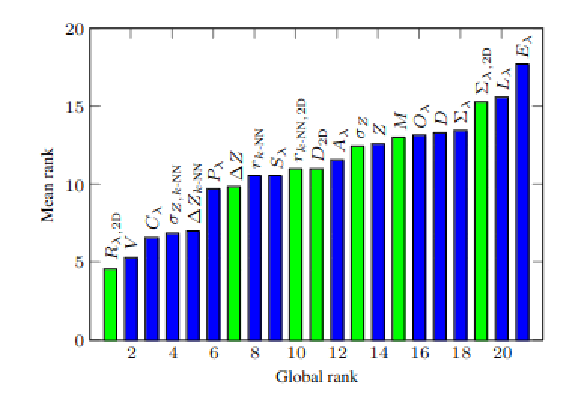
\includegraphics[width=0.6\linewidth]{97_graphics/related_work/geometric_features_ranking.pdf}
    \caption{Mean ranking of the derived features - 3D by blue and 2D by green \parencite{weinmann2013feature}}
    \label{fig:realted_work-3dgeo_feature_assessment}
\end{figure}

Various measures like F-score, Gini Index, Information Gain, Pearson correlation coefficient, and ReliefF were considered from the training data for the ranking of features. From the features ranking as shown in figure \ref{fig:realted_work-3dgeo_feature_assessment}, \( R_{\lambda,2D} \), V and \(C_{\lambda} \) are the most prominent features. \( R_{\lambda,2D} \) is a robust feature for detecting the exterior of the building, the verticality V is a promising feature in differentiating facades from the ground, and \(C_{\lambda} \) is a powerful feature in understanding the difference between planar and non-planar structures \parencite{weinmann2013feature}. Among the prominent features, an in-depth review of surface variation \((C_{\lambda}) \) is explained.

\subsubsection{Surface Variation}

\begin{figure}[htbp]
    \centering
    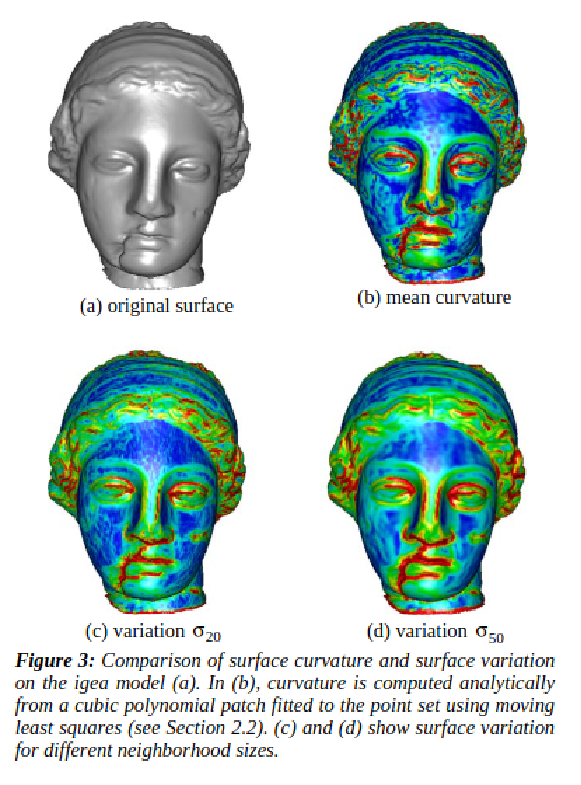
\includegraphics[width=0.6\linewidth]{97_graphics/related_work/surf_variation_with_description.pdf}
    \caption{Visualization of Surface Variation, referenced from \parencite{pauly2002efficient}}
    \label{fig:related_work-surface_variation_visualize}
\end{figure}

As shown in equation \ref{eq:surf_var}, surface variation, also known as surface roughness or surface irregularity, is the ratio between the minimum eigenvalue and the sum of eigenvalues. The surface variation of a point centered in a local neighborhood gives the change in curvature. This feature is invariant to scaling. A smaller value of the surface variation for that point indicates that all points in the local neighborhood lie on a tangential plane to the surface. The value of the surface variation of a point is dependent on the selected neighborhood. The selected neighboring point influences the covariance matrix, which influences the eigenvalues and hence the surface variation is varied. If \(C_{\lambda} = 0 \), then all the points of the neighborhood are located in the plane. \(C_{\lambda} = \frac{1}{3} \) is considered to be the value of isotropically distributed points \parencite{pauly2002efficient}. Figure \ref{fig:related_work-surface_variation_visualize} shows the variation of features for an Igea model. Various applications are possible by the analysis of surface variation such as quality control in manufacturing, surface reconstruction, designing components, etc.

\section{Surface Reconstruction}
The process of turning a collection of discrete points or a point cloud into a digital representation of an uninterrupted surface is known as surface reconstruction. It is essential in computer vision, computer graphics, and geometric modeling because it makes it possible to create 3D models from the real-world data that is acquired by sensors like depth cameras, LiDAR scanners, or other photogrammetry methods. Among various available methods for surface reconstruction, three are discussed.

\subsection{Alpha Shapes}
Alpha shape as explained in \parencite{edelsbrunner1983shape}, is the generalization of a convex hull. As clarified on \parencite{alpha_shapes_stanford}, \(\alpha-shape\) can be described as follows. Envision a massive ice cream mass forming a region, with the "hard" chocolate chunks represented as points on the region. All the areas of the ice cream mass are carved out that can be reached without running into pieces of chocolate by using ice cream spoons shaped in the form of a sphere. As a result, we even create holes inside the block (i.e., portions that are not accessible by just sliding the spoon from the outside). Eventually, what we have will be an object surrounded by caps, arcs, and points, but not necessarily convex.  The \(\alpha-shape\) of the points(chocolate toppings) could be understood by adjusting all the  "round" faces into triangles and line segments. \(\alpha\) in \(\alpha-shape\) represents the radius of the carving spoon, which determines the level of detail of the constructed surface. A higher value of alpha results in larger and simpler shapes with lower details. A lower value of alpha results in shapes with finer details. In figure \ref{fig:related_work-alpha_shapes}, points represent chocolate toppings and circles represent spherical ice-cream spoons in 2D space.

\begin{figure}[htbp]
    \centering
    \begin{minipage}[b]{0.45\textwidth}
    \centering
    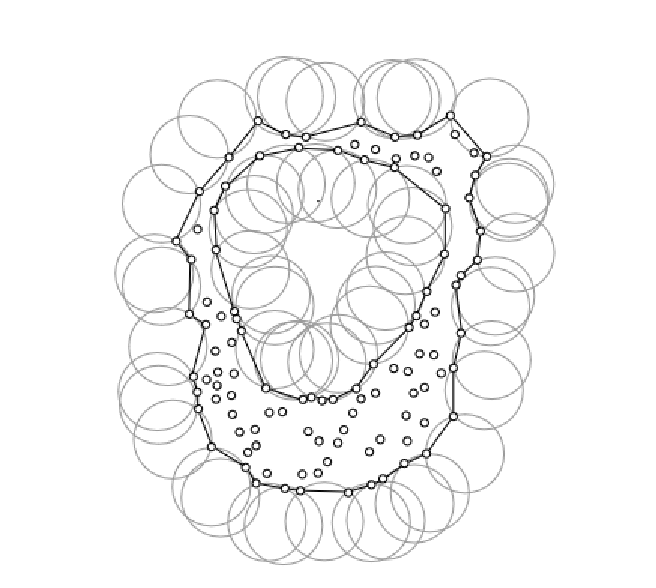
\includegraphics[width=1\linewidth]{97_graphics/related_work/alpha_shapes.pdf}
    \caption{Alpha Shapes Surface Reconstruction Method \parencite{alpha_shapes_stanford} }
    \label{fig:related_work-alpha_shapes}
    \end{minipage}
    \hfill
    \begin{minipage}[b]{0.45\textwidth}
    \centering
    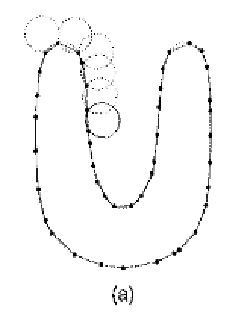
\includegraphics[width=1\linewidth]{97_graphics/related_work/ball_pivoting.pdf}
    \caption{Ball Pivoting Algorithm \parencite{bernardini1999ball}}
    \label{fig:related_work-ball_piv_3}
    \end{minipage}
\end{figure}


\subsection{Ball Pivoting}
Triangle mesh is constructed using the Ball Pivoting algorithm from a set of points \parencite{bernardini1999ball}. The idea behind the ball algorithm is straightforward. Starting from a single edge of the points in the unstructured points, a ball of a specified radius is moved or pivoted without leaving contact with the edge. A single triangle is formed if the ball touches three points, without considering any other points and without falling through. This process is carried on until all reachable edges have been tried. This process can also be viewed in figure \ref{fig:related_work-ball_piv_3}. Ball size can be varied to handle the varying point densities. For example, a larger-sized ball can be used to handle points that are very sparse.

\subsection{Poisson Surface Reconstruction}
By solving a regularized optimization problem, the Poisson surface regeneration approach produces a smooth surface \parencite{kazhdan2006poisson}. Because of this, this method for surface regeneration can be superior to the previously discussed techniques, which results in non-smooth outcomes because the points of the raw point cloud are also the location of the vertex of the final triangle mesh without any change. 

\begin{figure}[htbp]
    \centering
    \begin{minipage}[b]{0.45\textwidth}
    \centering
    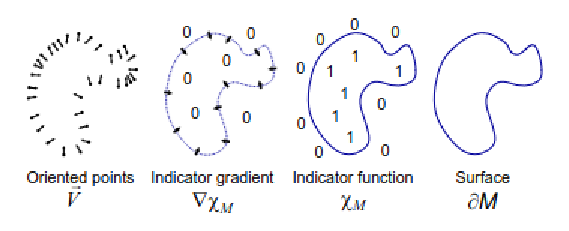
\includegraphics[width=1\linewidth]{97_graphics/related_work/poisson_reconstruction_2.pdf}
    \caption{Poisson reconstruction illustrated in 2D \parencite{kazhdan2006poisson}.}
    \label{fig:related_work-poiss_rec_2}
    \end{minipage}
    \hfill
    \begin{minipage}[b]{0.45\textwidth}
    \centering
    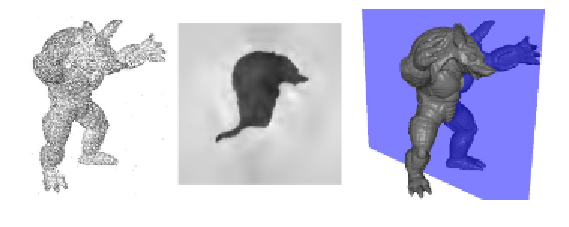
\includegraphics[width=1\linewidth]{97_graphics/related_work/poisson_reconstruction_1.pdf}
    \caption{Poisson Reconstruction illustration.\parencite{kazhdan2006poisson}}
    \label{fig:related_work-poiss_rec_1}
    \end{minipage}
\end{figure}

A model's indicator function and the oriented points, as shown in figure \ref{fig:related_work-poiss_rec_2}, that are collected from its surface are inextricably linked. In particular, the slope of the indicator function is a vector field that is equivalent to the inner surface normal nearly throughout (because the indicator function remains unchanged in almost every place), except in places that are close to the surface. Consequently, the directed point specimens can be considered instances regarding the model's indicator function gradient. Additionally, the indication function can be seen along the plane shown in the figure \ref{fig:related_work-poiss_rec_1} rightmost image and can be viewed by the middle image of the same figure in black color. Triangle meshes are constructed even in low-point density locations and also infer the surface in such locations. The density value of each point indicates if the neighborhood of the point is crowded by other points. Maximum tree depth for the octree defines the resolution of the final reconstructed triangle meshes.

\begin{figure}[htbp]
    \centering
    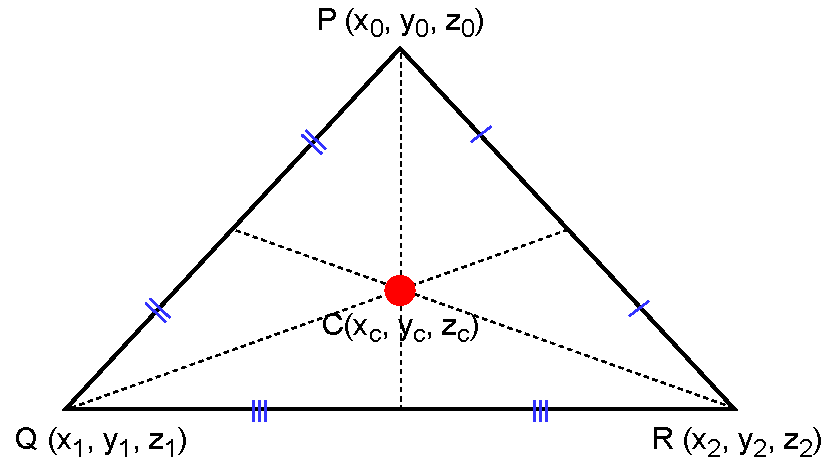
\includegraphics[width=0.5\linewidth]{97_graphics//related_work/centroid_of_triangle.pdf}
    \caption{Centroid of Triangle}
    \label{fig:basics-centroid_of_triangle}
\end{figure}

The reconstructed surfaces represent triangle mesh. For each triangle in the triangle mesh, the centroid can be calculated. Centroid refers to the center of the geometry. It can be thought of as the location where a geometry with an evenly dispersed mass could rest ideally on a needle spike. 
For $\triangle PQR$ as shown in figure \ref{fig:basics-centroid_of_triangle}, point "C" represents the centroid where the line bisecting the surfaces of the triangle intersects. The vertex of the triangle $\triangle PQR$ is represented by \(P(x_0, y_0, z_0)\), \(Q(x_1, y_1, z_1)\) and \(R(x_2, y_2, z_2)\). Centroid \(C(x_c, y_c, z_c)\) can be calculated using the equation \ref{equ:centroid_of_triangle}

\begin{equation}
    C(x_{\text{c}}, y_{\text{c}}, z_{\text{c}}) = \left( \frac{x_0 + x_1 + x_2}{3}, \frac{y_0 + y_1 + y_2}{3}, \frac{z_0 + z_1 + z_2}{3} \right)
    \label{equ:centroid_of_triangle}
\end{equation}

\section{Hidden Point Removal Algorithm}
The "Hidden" Point Removal operator \parencite{katz2007}is used to identify the points in a point cloud that are observable when perceived from a specific angle. Even in the absence of recreating a surface or measuring normals, visibility is ascertained.  This operator can be used on point clouds of different sizes, on sparse and thick point clouds, and on views both inside and outside the cloud. This algorithm is helpful for shadow casting, view-dependent reconstruction, and point cloud visualization. No point is genuinely hidden since points cannot obscure each other (unless they happen to fall along the exact same beam from the viewer). It is possible to identify which points are visible once a surface has been rebuilt from the points. This suggests that the cloud of points has information inherent to it that can be used to extract the point's visibility. Using the intrinsic information of points in the point cloud, the visibility of the points is determined without the need for surface reconstruction. For a point cloud with n number of points, the time complexity of the algorithm is \(O(n\log(n))\) \parencite{katz2007}.

For a point cloud with a "P" number of points, to find the points that are visible from a given viewpoint "C", the \acrshort{hpr} operator can be used. This HPR operator consists of two main steps as shown in figure \ref{fig:realted_work-hpr}. First is Spherical Flipping and second is the creation of a convex hull. 

\subsection{Spherical Flipping}
This step is also called inversion of points. The point "P" is in the geometry where the viewpoint is the Origin of the geometry. A function that maps a point \(p_i\) along the direction of the ray from the viewpoint and is declining in \(||\mathbf{p}_i||\) monotonically, results in spherical flipping. It can be given by equation \ref{eq:spherical_flipping}. Where \(\hat{\mathbf{p}}_i \) is the point after spherical flipping of point \(p_i\). \(R\) is the radius of the sphere and \(||\mathbf{p}_i||\) represents euclidean norm or magnitude of vector \(p_i\).

\begin{equation}\label{eq:spherical_flipping}
\hat{\mathbf{p}}_i = f(\mathbf{p}_i) = \mathbf{p}_i + 2(R - ||\mathbf{p}_i||) \frac{\mathbf{p}_i}{||\mathbf{p}_i||}
\end{equation}


\begin{figure}[htbp]
    \centering
    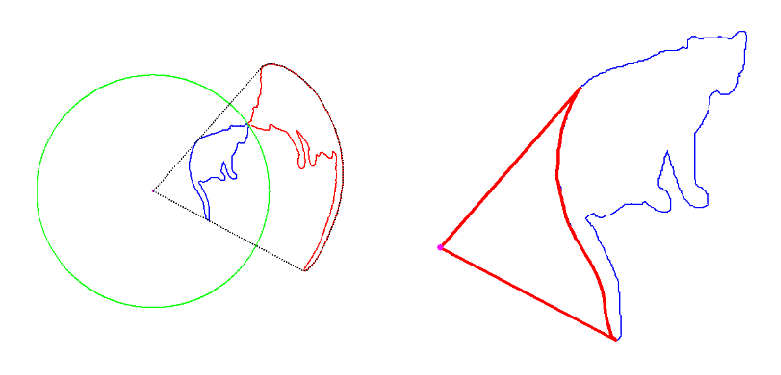
\includegraphics[width=0.5\linewidth]{97_graphics/related_work/spherical_flipping.pdf}
    \caption{Spherical Flipping and Back Projection\parencite{katz2007}}
    \label{fig:related_work-spherical_flipping}
\end{figure}

In the figure \ref{fig:related_work-spherical_flipping}, the green circle represents the Sphere whose center is the viewpoint C or Origin. For a noisy point cloud, the possible alternatives for the radius of the sphere can be found in \parencite{mehra_visibility_XXXX}. Blue curves, internal to the sphere, are projected along the ray from the viewpoint of its image external to the sphere.  This is represented by the red curve on the left side image of figure \ref{fig:related_work-spherical_flipping}. The right image of the figure represents the back project of the convex hull by the red-colored curve.

\begin{figure}[htb]
    \centering
    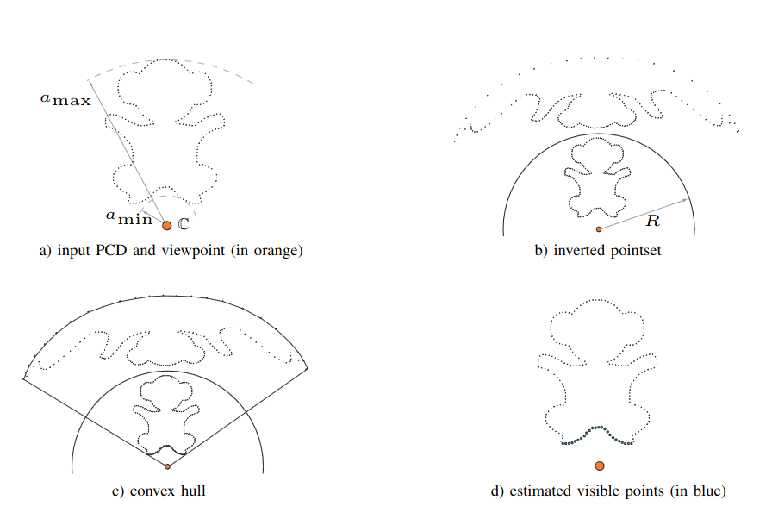
\includegraphics[width=0.8\linewidth]{97_graphics/related_work/hpr_2.pdf}
    \caption{Steps in HPR Algorithm \parencite{mehra_visibility_XXXX}}
    \label{fig:realted_work-hpr}
\end{figure}

\subsection{Calculation of Convex Hull}
In the next step of \acrshort{hpr}, the convex hull of the transformed point \(\hat{\mathbf{p}}_i \) is calculated. The transformed point cloud and the center of viewpoint are used to calculate the convex hull. Visibility of the point \(\hat{\mathbf{p}}_i \) is determined using the location of points respective to the convex hull. According to the algorithm, all the points are visible if the transformed points are located on the convex hull. Selection of the viewpoint C is crucial in the creation of a convex hull because, when C is external to P, points on the object's back may otherwise sit on the convex hull. The two steps can also be viewed in figure \ref{fig:realted_work-hpr}.

\section{Performance Metrices}
\subsection{Confusion Matrix}
The confusion matrix is the foundation of quality assessment matrices. It is a table that combines the test datasets' actual and anticipated values. Confusion matrices are typically employed for classification models and are used to determine the accuracy and correctness of the model. The projected classifications are in rows, and the actual ones are in columns. It is possible to switch the order of the anticipated and actual columns. In the figure, the positive class refers to the "YES" category, and the negative class refers to the "NO" category.

\begin{figure}[htbp]
    \centering
    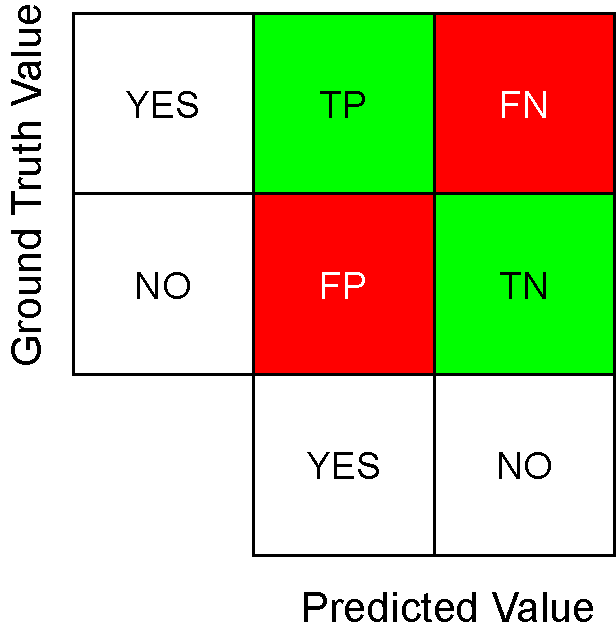
\includegraphics[width=0.5\linewidth]{97_graphics//related_work/conf_matrix.pdf}
    \caption{Confusion Matrix}
    \label{fig:related_work-conf_matrix}
\end{figure}

\begin{itemize}
    \item \textbf{\acrfull{tp} : } If the predicted positive value is the correct classification, these are TP.
    \item \textbf{\acrfull{tn} : }  If the predicted negative value is the correct classification, these are TN.
    \item \textbf{\acrfull{fp} / Type I Error : } For any classification task, if the positive class was predicted which is the incorrect classification. These are FP.
    \item \textbf{\acrfull{fn} / Type II Error : } For any classification task, if the negative class was predicted which is incorrect classification. These are FN.
    \item \textbf{Accuracy : } Tells about the percentage of correct predictions made by the model. Accuracy can be utilized as a benchmark to assess a classification model's performance in a balanced dataset; however, if the dataset is imbalanced (i.e., there is a significant actual difference in the number of positive and negative examples) then choosing a classification model based solely on accuracy is misleading.
    \begin{equation} \label{eq:accuracy}
        Accuracy = \frac{\sum TP + \sum TN}{\sum TP + \sum TN + \sum FP + \sum FN}
    \end{equation}
    \item \textbf{Precision}: The precision of a classifying model indicates the fraction of positively anticipated data that it could correctly identify as positive. Positive Predicted Rate is another name for it.
    \begin{equation}\label{eq:precision}
        \text{Precision} = \frac{\sum TP}{\sum TP + \sum FP}
    \end{equation}
    
    \item \textbf{Recall}: It provides us with the percentage of real positive cases that our algorithm was able to accurately anticipate. True Positive Rate or sensitivity are other terms for recall. A higher recall score indicates that our algorithm can accurately anticipate the majority of positive classes. A lower recall score indicates an inability of our model to accurately forecast the real positive examples.
    \begin{equation}\label{eq:recall}
        \text{Recall} = \frac{\sum TP}{\sum TP + \sum FN}
    \end{equation}
    
    \item \textbf{F1 Score}: A model's accuracy can be determined by calculating the F1-score, which takes into account both the precision and recall of the model's predictions. When working with unbalanced datasets or when the costs associated with false positives and false negatives differ, it is especially helpful. It is the harmonic mean calculated between precision and recall. The best case value of f1-score is 1 and the worst case value is 0. Optimizing recall and precision at the same time increases the value of the f1-score.
    \begin{equation}\label{eq:f1-score}
        \text{F1 Score} = 2 \times \frac{\text{Precision} \times \text{Recall}}{\text{Precision} + \text{Recall}}
    \end{equation}
\end{itemize}


Let's discuss the concept of performance metrics with an example. Consider a HAD system that needs to detect between a person and not a person. Out of 100 observations, 97 observations do not contain a person, and the remaining 3 observations contain a person. If predicting a person is a positive class and predicting a non-person is a negative class, then the metrics can be evaluated. If the HAD system predicted all the 100 observations as non-person then we have \(TP = 0\), \(TN = 97\), \(FP = 0\), and \(FN = 3\). We get an \(Accuracy = 97\%\). Because the dataset is unbalanced, as the number of positive and negative classes is not comparable, considering Accuracy as the determining factor is misleading. So options like F1-Score, Precision, and Recall should be further analysed.

\subsection{Intersection over Union}
\acrfull{iou}, also known as the Jaccard Index, is used to compare how similar two irregular shapes are to one another. It is a performance metric that is used to assess how well object detection algorithms perform, especially when it comes to computer vision and machine learning applications. By assessing the regions of overlap between the anticipated and ground truth bounding boxes, an object detection algorithm's accuracy can be determined. It can be calculated using the equation \ref{eq:iou}. IoU is also utilized in \acrfull{nms}. It is a post-processing method for object detection that helps to choose the most pertinent detected items by removing duplicate detections. A predicted bounding box with a higher IoU has maximum confidence in detecting the object and based on thresholding the IoU value, suitable predictions are finalized.

\begin{equation}\label{eq:iou}
    IoU = \frac{\text{Region of Intersection}}{\text{Region of Union}}
\end{equation}

\begin{figure}[htb]
    \centering
    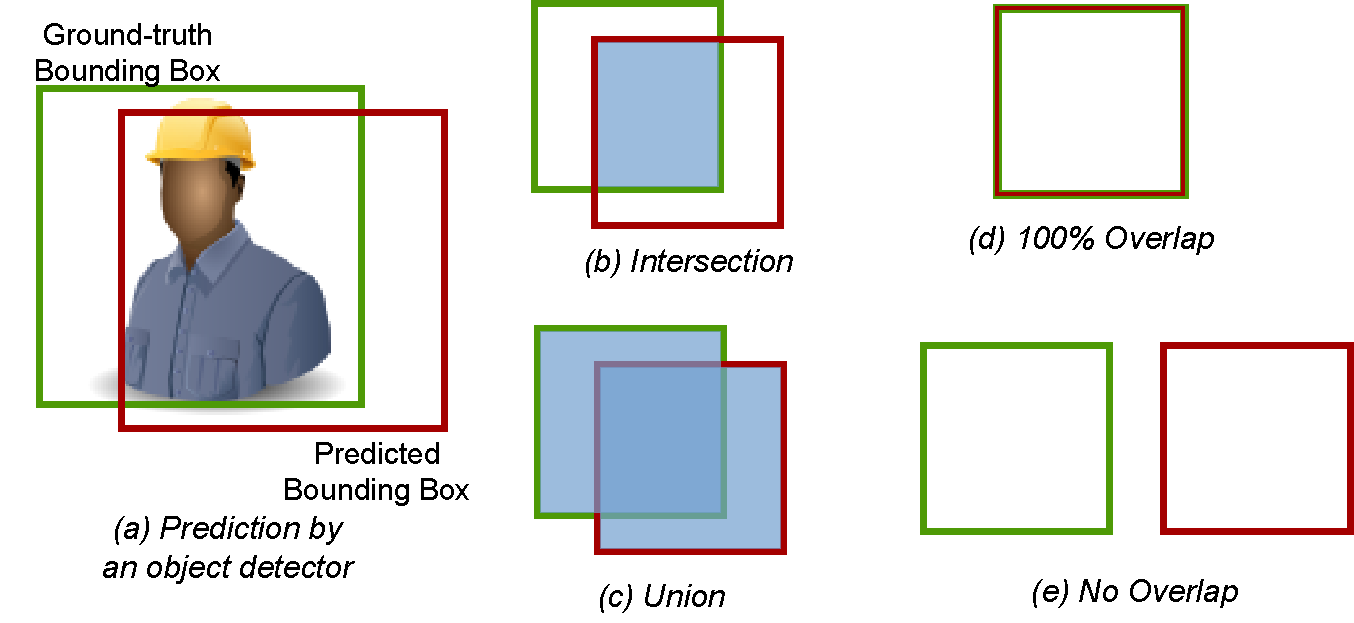
\includegraphics[width=1\linewidth]{97_graphics//related_work/iou.pdf}
    \caption{Intersection over Union}
    \label{fig:related_work-iou}
\end{figure}

Example image (a) in figure \ref{fig:related_work-iou} shows the result of an object detection algorithm. The green colored box is the ground truth and the red colored box is the prediction by the algorithm. By calculating the area of intersection and area of union between the two boxes, IoU can be calculated. Image (d) represents completely overlapped bounding boxes. The IoU in such a case is 1. In case of no overlap between the two regions  (image (e)), the IoU is 0. It is necessary to select an accuracy threshold when utilizing IoU as an evaluation metric. Based on the threshold, the result from an algorithm can be either accepted or rejected.

			\chapter{Related Work}
The \acrfull{ecu} of the \acrshort{had} system are in charge of comprehending the environment and making the right decisions. To accomplish high-level tasks like course planning and collision avoidance, the \acrshort{had} system has to estimate a more detailed 3D bounding box within the real world. The fundamental part of the ECUs that manages perception, judgment, route planning, etc. is the  \acrfull{dnn}. The quantity and quality of annotated training data are the primary determinants of DNN performance. The main issue that arises while training a DNN based on point clouds is the scarcity of ground truths, which severely restricts the network's ability to converge quickly and perform at its best. More data is required for DNN to reduce the problem of class imbalance, enhance generalization, and prevent overfitting of the model.

One interesting approach that makes it simple to collect all ground truth labels is synthetic data simulation. Utilizing computer graphics techniques, efforts have been made to produce artificially labeled data \parencite{SuQLG15, 8462926, abs-1809-08495}.  Using the video game engine's APIs from Grand Theft Auto V (GTA-V), \parencite{abs-1804-00103} gathers the calibrated pictures and point cloud and uses this information for vehicle recognition in subsequent projects \parencite{8462926}. Simulators like AutonoVi-Sim, \acrshort{carla}  \parencite{8575306, Dosovitskiy17} are also employed for purely synthetic data generation. The \acrlong{cg} world has a restricted scale and complexity and is primarily created by hand. Although it is demonstrated that using these simulated data might enhance DNN performance, there are still certain issues like domain gaps\parencite{zero_domain_gap, care_real_and_syn_gap} that need to be resolved. 

\section{Data Augmentation}
\acrfull{da} has been extensively investigated for 2D images \parencite{transfsim2000, NIPS2000_ba9a56ce} and has shown enormous possibilities in training effective \acrshort{dnn} models with restricted training images. \acrshort{da} tries to modify and create new training samples in order to extend the variety of the training data. \parencite{xiao2022polarmix} . \acrshort{da} has been a standard pre-processing step when training a neural network, as its efficacy has been demonstrated across a wide range of tasks \parencite{lidar_aug, second2018, pointmixup2020}. In \parencite{abs-1708-01566}, the real-world image dataset is enhanced by the addition of rendered automobiles, which benefits from the foreground's variance and the background's realism. For the 2D image domain, several data augmentation methods are covered. In Cutout \parencite{cutout}, sections from images are taken off to enhance an image patch. MixUp \parencite{mixup} combines two images and the corresponding labels. CutMix \parencite{cutmix} is a technique that replaces a part of an image with a patch from another image, combining Cutout and MixUp. Though many efforts have been made on image augmentation, very few concentrate on point cloud data augmentation.

\parencite{DBLP:journals/corr/abs-2004-01643} delves into a variety of augmentation strategies, such as global augmentation, local augmentation, GT-filtering, and GT-sampling, to enhance data diversity in 3D point clouds. While local augmentation methods are specific to the points associated with certain objects in the scene, global augmentation strategies work on the point cloud representing the whole scene.
Global augmentations are applied concurrently to every point in the point clouds and every annotation. Several methods, including global translation, rotation, scaling, random flipping, and ground removal, are included in global augmentation. In contrast to global augmentation, local augmentation techniques also involve translation, rotation, and scaling. However, the key distinction lies in their application: rather than applying these transformations to every point indiscriminately, they are only used with specific labels and the points that are included in those labels. By using distinct random values for every label class, this method guarantees that each label class is enhanced individualistically from the others.
The GT-Filtering method serves as a means to filter ground truth objects. This filtering process can be contingent upon various factors, such as difficulty level (difficulty level as described in KITTI \parencite{Geiger2012CVPR}) or the extent of points contained within the objects. The practice of incorporating more reference instances, such as individuals, from other scenes into the present scene is known as GT-Sampling. In order to do this, a database linking class labels to points must be created and all labels must be reprised over once. This strategy is used to rectify the disparity between the "background" and "foreground" in datasets like SemanticKITTI \parencite{behley2019semantickitti}, thereby aiming for more balanced datasets. The subsequent section delves into various LiDAR augmentation strategies, exploring methods to enhance LiDAR data for improved performance in tasks such as object detection, segmentation, and classification.

\section{Augmentation Strategies involving LiDAR point cloud}

This section provides a detailed examination of different augmentation strategies concerning LiDAR point clouds. The emphasis is placed on elucidating the key features and characteristics of each strategy, delineating their significance in enhancing the quality and diversity of LiDAR data for various applications. 
\begin{itemize}
    \item \textbf{SECOND: Sparsely Embedded Convolution Detection} : In this study \parencite{second2018}, a database was constructed to store the labels of all reference (\acrshort{gt}) objects and their corresponding point cloud data derived from the training dataset's 3D bounding boxes. Throughout the learning process, a subset of ground truth objects was arbitrarily chosen from this repository using GT-Sampling methodology and integrated into the present training point cloud by using the join operation. This augmentation strategy aimed to augment the number of \acrshort{gt} reference objects per point cloud, thus facilitating the simulation of objects prevalent in varied surrounding conditions. Consequently, the detection performance was enhanced; nevertheless, it was observed that the methodology failed to consider the obstruction interaction that exists between various enhanced objects as well as among surrounding regions and enhanced objects, thereby disregarding the importance of rational placement and occlusion considerations. Overall, the augmentation technique primarily relied on the simple reuse of ground truth objects.
    \item \textbf{Mix3D} : In this methodology \parencite{mix3d2021}, several augmentation techniques is employed to enhance the diversity and robustness of the LiDAR point cloud data. Firstly, the translation of multiple scenes to the origin was carried out by subtracting the centroid from all point positions, ensuring uniformity in spatial orientation. Subsequently, random transformations such as flipping in both horizontal directions and random rotations along different axes is applied to introduce variability. Additionally, random sub-sampling, elastic distortion, and random scaling is implemented, along with possible contrast augmentation, random brightness adjustments, and color jittering. Post-augmentation, the augmented point clouds from both scenes is merged by simply combining their points, effectively forming the union of the two sets. Furthermore, to augment the data out-of-context, points from two scenes is concatenated, serving as a valuable augmentation strategy, particularly useful for tasks like semantic segmentation.
    \item \textbf{LiDAR-Aug} : This research endeavor \parencite{lidar_aug}, introduces a rendering-based framework specifically designed to augment LiDAR point cloud data. The automatic implementation of obstruction impediment is ensured by the seamless integration of supplemented elements into genuine background scenes through the utilization of rendering methodologies. Furthermore, a novel method is proposed for incorporating \acrfull{cad} models into scenes and generating augmented LiDAR point clouds using a rendering module. The framework also employs the lightweight "ValidMap" strategy to impose stances for the supplemented objects, ensuring collision avoidance and achieving realistic obstruction insertion. Moreover, improvements are made over GT sampling by implementing measures to avoid object collisions during the object insertion process.
    \item \textbf{Augmented LiDAR Simulator for Autonomous Driving} : This study \parencite{aug_lidar_sim_2020} presents a LiDAR point cloud simulation framework  designed to enrich real point clouds by incorporating synthetic obstacles. The synthetic obstacles, represented by movable \acrshort{cad} models, encompass various types, with 500 models dedicated to pedestrians, 45 models allocated for cars, SUVs, etc. Real-world background models acquired using the RIEGL scan device, renowned for its high-speed, high-performance dual scanner mobile mapping system capabilities, are seamlessly integrated with semantic information. Background annotation using semantic segmentation information obtained through PointNet++ \parencite{pointnetplus2017} is employed, with annotations meticulously refined through filtration by groups of annotators. Additionally, the framework incorporates realistic obstacle placement learned from real traffic scenes to ensure the authenticity and accuracy of the augmented point cloud environment.
    \item \textbf{LiDARsim} : In this simulation-based approach \parencite{lidarsim2020}, the scan background is substituted with a method involving registration techniques for LiDAR and diverse frames aggregation, while dynamic objects are regenerated out of \acrshort{pcd} data rather than relying on artificial \acrshort{cad} models. To facilitate this, a substantial catalog comprising 3D static maps and dynamic objects is first compiled through extensive drives across different cities with the self-driving fleet. Scenarios are subsequently generated by selecting scenes from this catalog and virtually placing a \acrfull{sdv} and dynamic objects within the chosen scenes, ensuring plausible and realistic arrangements.
    \item \textbf{PointMixup} : PointMixup \parencite{pointmixup2020} introduces an interpolation method influenced by MixUp \parencite{mixup} in image enhancement strategy. This approach discovers novel instances by efficiently assigning the path function between the labeled training \acrshort{pcd}s.
    \item \textbf{PointAugment} : This approach \parencite{pointaugment2020}is utilized for automatically optimizing and augmenting point cloud samples during the training of classification networks through the use of an augmentor to enhance data diversity. This method is employed to learn augmentation functions tailored to individual samples or classes, ensuring specificity in augmentation strategies. This approach integrates sample-aware auto-augmentation techniques and incorporates objectwise augmentor learning alongside classification learning using labeled training samples. However, the inclusion of an additional augmentor network and the intricate adversarial training process may introduce practical challenges to implementation.
    \item \textbf{PointPainting} : The proposed approach \parencite{pointpainting2019} involves initially executing the camera image through an image categorization algorithm. Subsequently, the anticipated categorization class grades are projected onto the LiDAR point cloud, effectively "painting" the point cloud with the segmentation results obtained from the camera image. This method offers an enhancement in 3D detection capabilities compared to the augmentation techniques.
    \item \textbf{PointAugmenting} : This research \parencite{pointaugmenting2021} introduces an object detection algorithm focusing on integrating 2D camera images with 3D LiDAR point clouds. In this methodology, deep features extracted by a 2D Object Detector from camera images are projected onto the corresponding points within the LiDAR point cloud. This process facilitates the fusion of information from the 2D image domain into the 3D LiDAR space, enhancing the feature representation and potentially improving object detection performance.
    \item \textbf{\acrfull{paaug}} : The proposed method \parencite{pa_aug2020} leverages the structural information of 3D ground-truth boxes to enable the network to learn intra-object relationships. It prolongs the GT-Sampling technique through creating sub-division within GT objects and introducing random augmentation to every division. Objects such as cars, cyclists, and pedestrians from the KITTI dataset are utilized for this purpose. By dividing objects into multiple partitions and probabilistically applying LiDAR data augmentation operations like dropout, swapping, mixing, sparsifying, and introducing noise to each partition region, the method not only enhances the accuracy of the dataset but also demonstrates robust performance on corrupted data.
    \item \textbf{Augmentation of LiDAR for Fog Simulation} : A novel fog simulation method suitable for any LiDAR dataset is discussed in \parencite{fog_sim_2021}, focusing on achieving physically valid simulations. This method involves augmenting clear weather point cloud data with artificial fog, thereby enhancing the realism of the dataset. The strategy has enhanced the efficacy of 3D object detection under challenging atmospheric conditions characterized by the presence of fog.
    \item \textbf{Augmentation of LiDAR for Snowfall Simulation} :\parencite{snow_sim_2022} discusses augmenting the LiDAR point cloud to simulate real-world snowfall. Using this method, artificial snow is added to clear weather point clouds. With this method, each LiDAR line's snow particle sample is taken in two dimensions, and the resulting geometry is used to modify the measurement for each LiDAR beam.
    \item \textbf{Patch-based Progressive 3D Point Set Upsampling} :  \parencite{patched_up_2018} discusses the method of upsampling from lower resolution points to enhance resolution, aiming to reveal detailed geometric structures from sparse and noisy inputs.
    \item \textbf{\acrfull{sessd}} : In the proposed methodology \parencite{sessd_2021}, the ground truth bounding box is partitioned into six pyramid shapes by connecting the centroid with the faces of the box. Subsequently, random dropout, swap, and sparsify operations are applied to each subset of points derived from these divisions, effectively simulating partial object occlusion, increasing object diversity, and mimicking variations in point sparsity. This process treats the divided point subsets as disassembled parts, allowing for targeted manipulation. Prior to shape-aware data augmentation, a series of global transformations are applied to the input point cloud, including random translation, flipping, and scaling. Overall, this approach integrates both shape-aware and global transformations to augment the data effectively.
    \item \textbf{\acrfull{ppba}} : PPBA \parencite{ppba_2020} uses automated data enhancement methods to find the ideal settings for augmentation. During this procedure, the augmentation schedule is optimized by reducing the size of the search space and using the most effective parameters from previous rounds. It is discussed that sampling from individual frames of data from sensors results in a tenfold gain in data efficiency.
    \item \textbf{\acrfull{dada}} :  \parencite{dada_2023} In this approach, transformation of orthogonal coordinates of the point cloud into a spherical coordinate system is carried out, followed by sampling based on the LiDAR characteristics specific to the dataset, such as Velodyne HDL-64E for KITTI \parencite{Geiger2012CVPR} or a 40-beam LiDAR for the ONCE dataset \parencite{mao2021one}. The object is evenly sliced and sampled in accordance with the LiDAR resolution corresponding to the dataset's LiDAR characteristics. In the case of existing ground truth (GT) objects, points are simulated while adhering to the LiDAR characteristics to maintain the object's shape. Subsequently, downsampling or upsampling is performed based on the point density requirements.
    \item \textbf{PolarMix} : This method \parencite{xiao2022polarmix} presents an innovative way to mix in cylindrical coordinates at the object and scene levels. Swapping at the scene level involves slicing along the azimuth axis to exchange point cloud regions of two circular LiDAR scans. Mixing at the instance level involves copying the rotated point objects into additional scans after cropping them from one LiDAR scan and rotating them by various azimuth degrees to make several copies. It should be noted, nevertheless, that this approach does not take shadowing effects into consideration and can lead to the illogical positioning of instance objects.
    \item \textbf{PatchAugment} : The focus of this methodology \parencite{patch_aug_2021} is on enhancing data inside the immediate area or neighborhood of the sampled object, which principle is similar to the \acrshort{paaug} data augmentation technique.
    \item \textbf{PointCutMix} : Inspired by \acrfull{msda} in the image domain, this method \parencite{pointcutmix_2021} generates new training data by mixing the original training samples. Specifically, subsets of point objects are replaced with those of other objects to enrich the training data. To utilize this approach, annotated point cloud objects from two point clouds with corresponding labels are required.
    \item \textbf{RS-Aug} : This approach \parencite{rs_aug_2023} involves constructing an augmented reality scene to enhance the diversity of the training dataset. Initially, a pre-trained semantic segmentation model, RangeNet++ \parencite{rangenetplus2019}, is utilized to estimate semantic labels. This step serves as a preprocessing stage for the creation of a database in the auto-annotation process. Subsequently, the database is sampled for rendering augmentation in the subsequent step.
    \item \textbf{\acrfull{br}} : In this approach \parencite{xu2022reality}, position-level annotation is employed to build a virtual scene using an existing object database, facilitating weakly supervised 3D object detection. This process entails labeling the center of each object in the 3D space, followed by generating a virtual scene from a repository of 3D shapes.
    \item \textbf{Object Insertion Based Data Augmentation for Semantic Segmentation} : In this research \parencite{9811816}, annotated LiDAR point clouds are used to extract foreground objects, which are then upsampled to create an object library. Objects are dynamically introduced into the LiDAR point cloud during training. Parameters similar to actual LiDAR settings are used to mimic realistic scanning lines and shadows by using range images, which are generated depending on the resolution of the LiDAR used for data gathering.
    \item \textbf{PointWOLF} : To enhance the variation of known 3D objects, this approach \parencite{pointwolf_2021} uses weighted alterations within local neighborhoods. It might be used, for example, on objects like wolves to produce different poses. The needed diversity is obtained by carefully combining several local transformations that are done with regard to anchor points in smoothly varied ways.
    \item \textbf{Real3D-Aug} : In this method \parencite{sebek2022real3daug}, objects are strategically placed at the same distance with identical observation angles to ensure consistent object point density and LiDAR intensity across the dataset. Additionally, collision avoidance measures are implemented by analyzing overlapping bounding boxes within semantic datasets.
    \item \textbf{Contextual Ground Truth Sampling} : In order to rectify data imbalances and insert ground truth \acrshort{gt} objects in realistic placements, this method \parencite{lee2022resolving} uses contextual GT sampling (sampling ground truth objects from a pre-saved GT database).
\end{itemize}

\section{Need of the Thesis work}

The majority of augmentation methods primarily aim to enhance model performance for detecting specific classes using pre-labeled class instances. Many existing strategies assume prior knowledge of ground truth objects, with some leveraging state-of-the-art semantic models to obtain this information \parencite{rs_aug_2023}. However, occlusions are often overlooked in some augmentation strategies \parencite{second2018, xiao2022polarmix}, and accurate 3D bounding boxes are typically required for appropriate object insertion into the scene. While some approaches utilize a database of rendered graphics models of objects \parencite{second2018, rs_aug_2023}, simulators often rely on CAD models, which may exhibit unrealistic appearances, necessitate costly manual construction, and lack scalability to represent the diversity and complexity of real-world scenarios. Additionally, certain augmentation methods require knowledge of the LiDAR configurations used for the target dataset to facilitate augmentation effectively \parencite{9811816, dada_2023}. 
Semantic segmentation of LiDAR frequently exhibits a decrease in accuracy when applied to LiDAR setups not previously encountered, as elucidated in \parencite{10204248}. This discrepancy results in an accuracy decline in LiDAR data-based semantic classification tasks when the LiDAR operated for gathering the evaluation set contradicts the LiDAR utilized for the learning set. The variance in sampling patterns across various LiDAR configurations, characterized by differences in vertical and horizontal resolution, contributes to the emergence of sensor bias issues in 3D perception algorithms \parencite{survery_domain_adp_2021, domain_adp_appr_2020}. 
Certain augmentation techniques, like PA-AUG and PointWolf, concentrate only on enhancing the ground truth (GT) objects, they do not handle how these objects are combined with the surrounding scene. 
Current augmentation strategies rely on either known labeled data or semantic models to extract ground truth objects. However, there could be situations where the label of the ground truth objects to be extracted is unknown. \acrshort{sota} semantic models may also prove ineffective, as the model may not have encountered the specific object during the training.
Even though the 3D semantic models have been trained on relevant objects before, using 3D semantic models is still ineffective as it requires an ideal model for the extraction of the specific object and the present \acrshort{sota} 3D Semantic Models performance (Mean \acrshort{iou}) on real-world datasets like SemanticKITTI is below 80\% \parencite{papers-with-code}.
This highlights the need for alternative approaches to handle scenarios where ground truth information is unavailable or difficult to obtain.


			\chapter{Concept}

We aim to manipulate the position of a \acrshort{vru} (i.e. prototype or person) within a point cloud without physically relocating objects(prototypes) in the real world. This process involves extracting the point cloud corresponding to a prototype by leveraging geometric characteristics of points in three-dimensional space, followed by transforming the prototype's point cloud to a specified location. This approach enables evaluation of the response of a 3D object detection model to different scenarios wherein the prototype is situated in varied locations or within distinct background point cloud scenarios.

In this project, we refer to the source scene cloud as the point cloud from where an object or prototype needs to be extracted. A prototype is an object or a part of the source scene cloud that represents the point cloud of an actual object or object of our interest (person or prototype). The prototype is later also referred to as the original prototype to indicate it has not undergone transformation. The target scene cloud is the cloud where we insert the extracted prototype cloud, creating a new scenario cloud. Generally, at a high level, the system consists of two major steps which consist of sub-steps. The first step is represented by prototype extraction, which is represented by green color in the figure \ref{fig:concept-graph}. In this step, the prototype is extracted from the source scene cloud. The second major step is called as recombining of points cloud that is represented by red color on the figure \ref{fig:concept-graph}. In this step, the prototype extracted from the source scene is merged or recombined with the target scene cloud. Further recalculation of the point cloud of the prototype and calculation of shadow casting on the target scene is done in this step. The result of the system is a target scene consisting of a prototype cloud that resembles as if there was an actual prototype object on the target scene in real world. In the following section, we discuss each step in detail.

\begin{figure}[htbp]
    \centering
    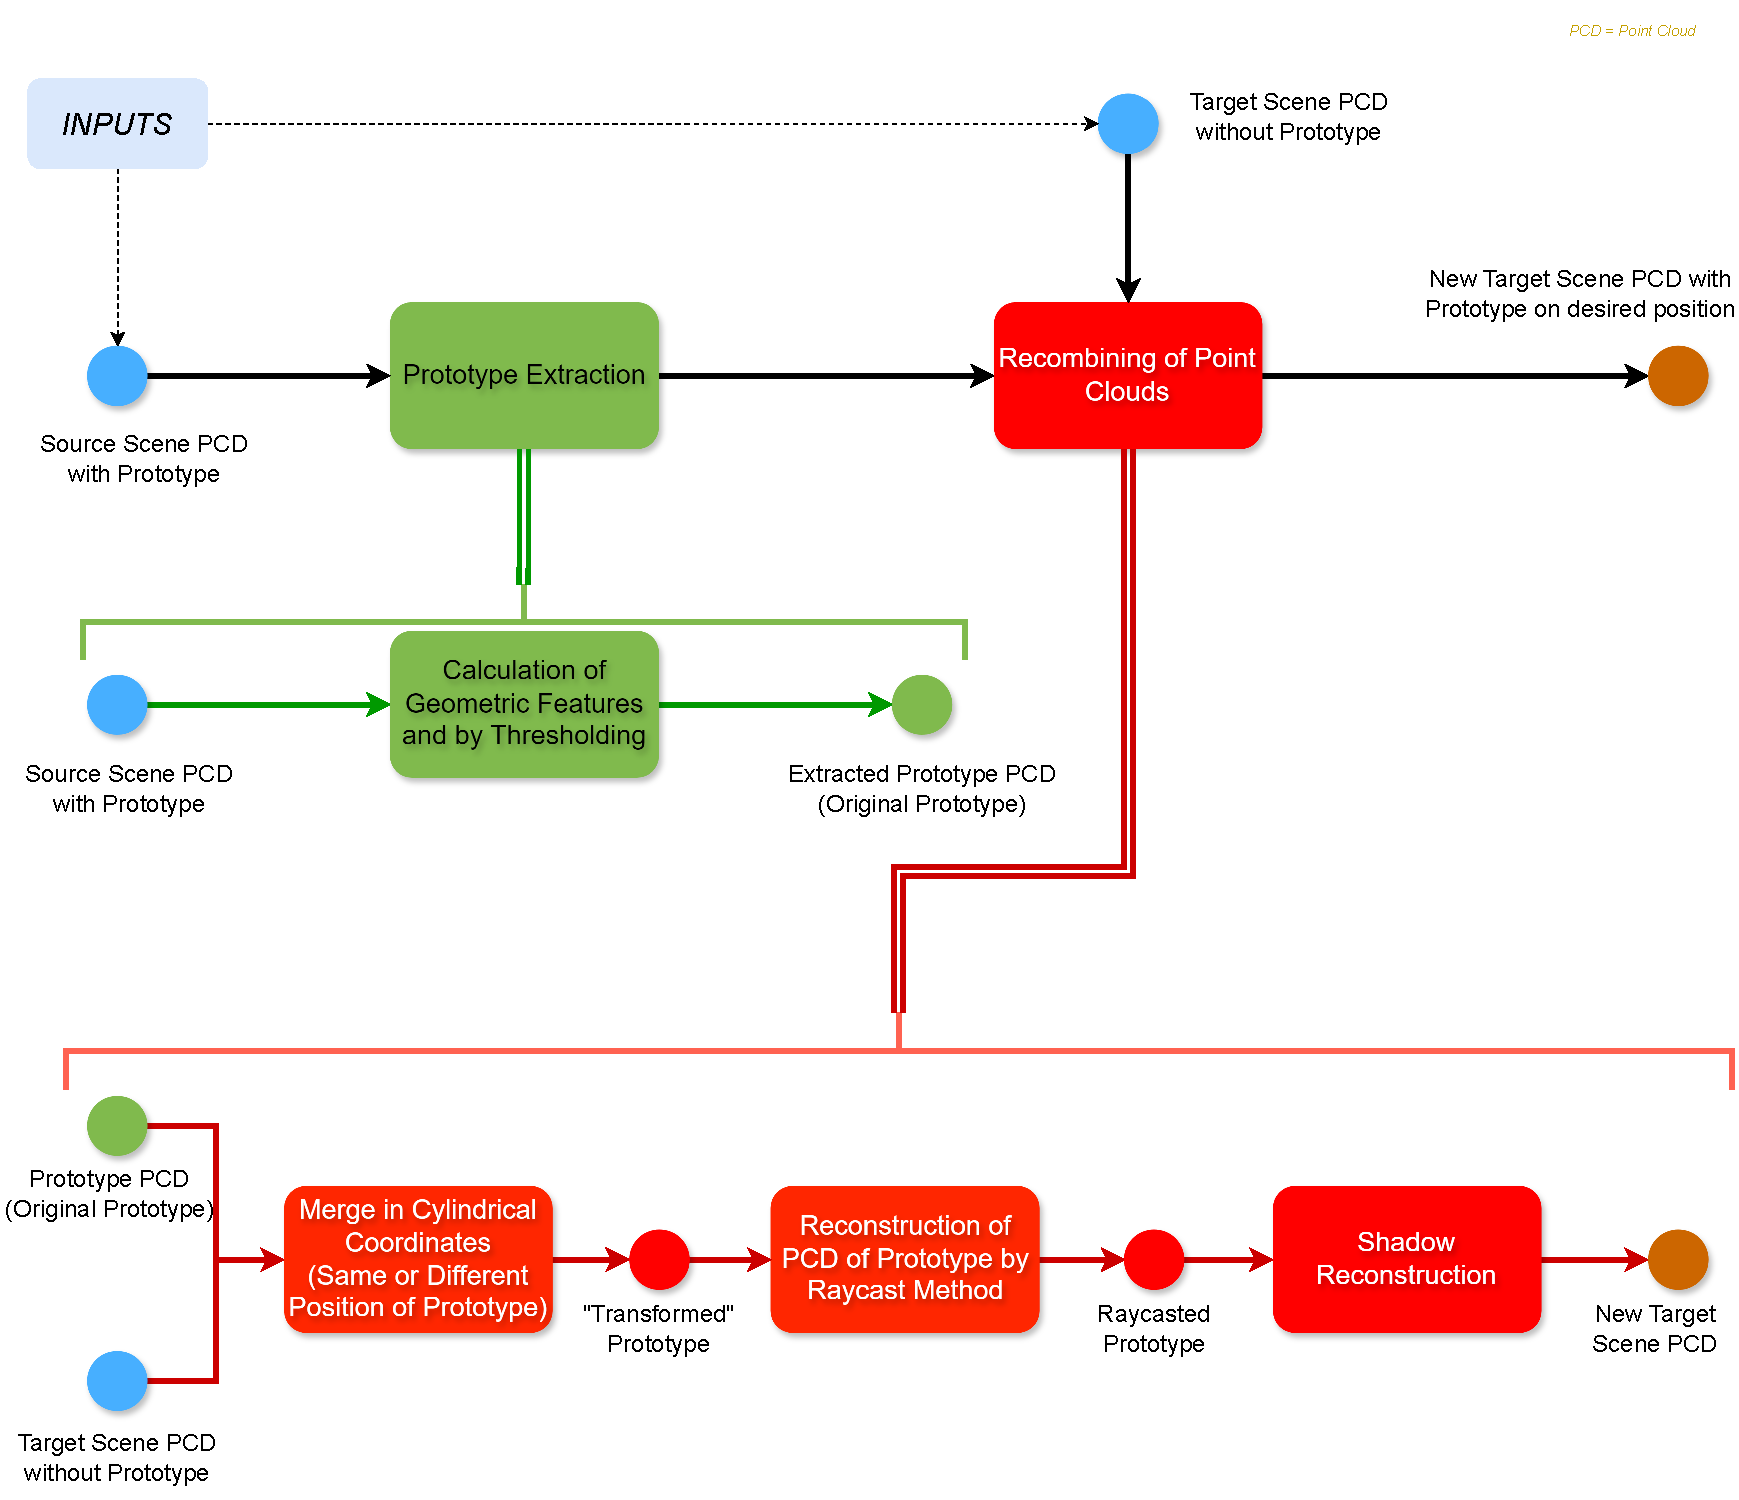
\includegraphics[width=1\linewidth]{97_graphics/concepts/graph_main.pdf}
    \caption{Concept graph representing the workflow of the project}
    \label{fig:concept-graph}
\end{figure}



\section{Prototype Extraction}
The thesis aim is to create new point clouds by extracting prototypes from one point cloud (source scene cloud) and placing the extracted prototype in a desired location on another point cloud (the target scene cloud). This facilitates the augmentation of an existing point cloud with additional objects or artifacts within the scene. Enabling such a process would increase the information content of the point cloud, which could be utilized to train various point cloud models or could be used to test the feasibility of a \acrshort{had} system that would act when the prototypes are situated on the positions.
We have multiple options for prototype extractions from the source scene cloud. To extract the prototype from a source scene cloud, we first select a region of interest from where we need to extract the prototype. For our project, we had mainly three options of prototype extractions from the region of interest of the source scene cloud. 
\begin{enumerate}
    \item Extraction of a prototype using known Labels
    \item Extraction of a prototype using semantic \acrshort{ml} models
    \item Extraction of a prototype using geometric features
\end{enumerate}

\subsection{Extraction of prototype using known Labels}
Given a source scene cloud, a prototype could be extracted from a source scene cloud using the known labels of the point cloud. There is one precondition that needs to be met before using this approach. The precondition is that the point cloud from where the prototype is to be extracted should be labeled. Also, the label of the prototype to be extracted should be known. If we know the label of the prototype on a labeled point cloud then it would be straightforward and a perfect way to extract the prototype from the source scene. However, this may not typically be the situation. Considering the time and cost effort required to get completely correct labeled data, most of the point cloud datasets available publicly online are just raw point clouds without labels. So choosing this approach is not feasible as a precondition has to be met before following this approach, which is not always the case. So we explored the next approach.

\subsection{Extraction of prototype using semantic ML models}
We also have an option of using state-of-the-art 3D semantic models for the extraction of prototypes. A semantic model from \parencite{Chen2022} could be used to extract prototypes from the source scene cloud. The source scene cloud does not need to be labeled for the extraction of the prototype. However, one precondition has to be met to use \acrfull{ml} models for the prototype extraction. The \acrshort{ml} model needs to be trained with the prototype-like objects and this requires a labeled dataset. Also, it requires an ideal semantic ML model to accurately extract the prototypes, which in the present context is not feasible. Considering the laborious task of point cloud data annotations and the requirement of an ideal semantic ML model, we explored next on a simple yet effective approach to prototype extraction using geometric features.

\subsection{Extraction of prototype using geometric features}
Geometric features such as surface variation, planarity, and linearity are used for this step to extract the prototype point cloud from a scene. We mainly focused on surface variation. Considering a part of the point cloud selected from a source scene, surface variation tells us the change in surface features for a selected neighborhood. For the goal of extracting a prototype from a region of interest, we mostly see an object standing on a flat surface. The roughness (surface variation) for the flat surface is low in comparison with the feature of the prototype to be extracted. This is because of the orientation of the points in the 3D space. Instead of calculating geometric features for a whole scene, we selected a region of interest where the prototype is located. Geometric features are calculated for the selected region of interest with appropriate parameters for the nearest neighbor search. Thus calculated geometric feature is filtered with appropriate values by trial and error. The result is an almost perfect extracted prototype. Thus we do not need to rely on known labels or on using \acrshort{sota} semantic 3D models for prototype extractions as for a selected \acrfull{roi}, just using the geometric features is also good enough. As a result, a prototype is extracted from the source scene cloud by thresholding the calculated geometric features. Thus extracted prototype will be combined with the target scene in the next step to generate new scenarios in the target scene cloud.

\section{Recombining of Point Clouds}
This step is represented by blocks with red color in the figure \ref{fig:concept-graph}. This stage involves the relocation of the prototype object to a specified target location within the target scene cloud. Subsequently, the point cloud associated with the prototype is recalculated based on its new position, followed by the computation of shadow casting projected by the transformed prototype. Each of these sub-steps can be described in detail below.

\subsection{Merge of Prototype and Target Scene Cloud}
The goal of this step is to place the extracted prototype on a selected region of the target scene cloud. Initially, experiments were done with registration algorithms like the \acrfull{icp} algorithm to find the optimal transformation of the prototype point cloud to the target location. This method proved to be ineffective, particularly in scenarios where we intend to relocate the prototype to a region within the target cloud characterized by sparse point density, such as areas distant from the origin of the point cloud. For the \acrshort{icp} algorithm to work, we need to have a set of correspondence between the points in the prototype cloud and the target scene cloud. 

\begin{figure}[htbp]
    \centering
    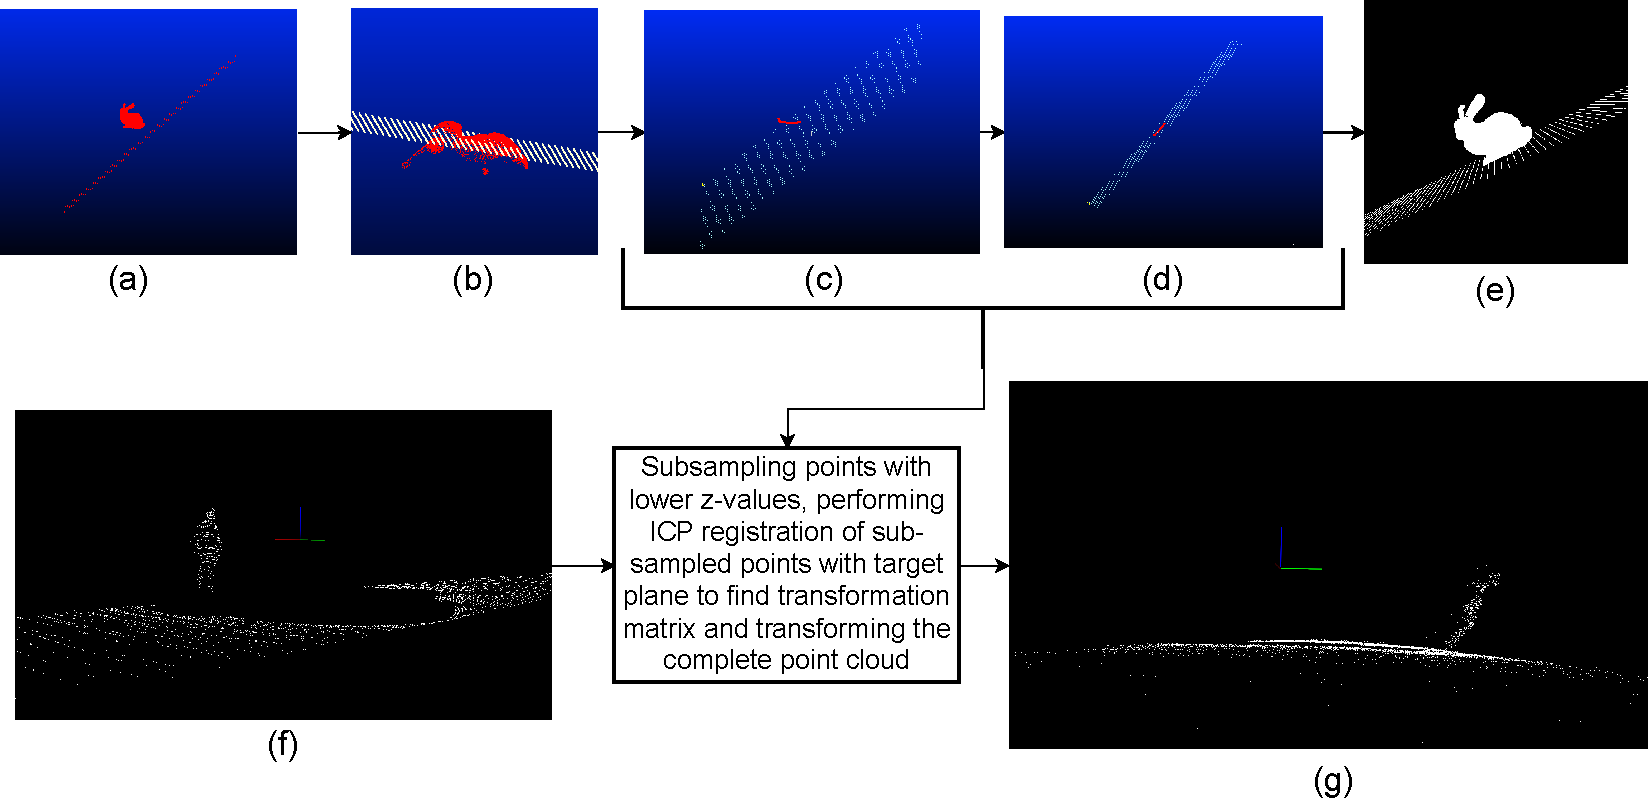
\includegraphics[width=1\linewidth]{97_graphics/concepts/icp_registration_analysis.pdf}
    \caption[Transformation of source cloud to target scene plane using \acrshort{icp} Registration Algorithm]{Transformation of source cloud to target scene plane using \acrshort{icp} Registration Algorithm (a)Bunny cloud needs to be placed on target inclined plane (b) Simple ICP registration with complete bunny cloud (c) Subsampling lower z-values points of bunny cloud (d) ICP registration of sampled points with the target plane (e) Bunny point cloud transformed using the transformation matrix calculated from subsampled ICP registration step (f) Point cloud of a person on a source scene (g) Point cloud of the person (inclined) after ICP registration on target scene cloud. } 
    \label{fig:icp_registration_analaysis}
\end{figure}

Taking the lower points of the prototype (i.e. points with lower z-values) as correspondence points on the target region works with the \acrshort{icp} algorithm as visualized in the upper row images in figure \ref{fig:icp_registration_analaysis}. But this step has a major drawback. This step assumes that the lower point(i.e. points with low z-values) of the prototype lies on the target region. This method fails to work if the point with lower z-values does not lie on the target location and is located slightly above the ground. This can be shown by the registration of the person point cloud in the bottom row images in figure \ref{fig:icp_registration_analaysis}.
As shown in figure \ref{fig:icp_registration_analaysis}, even though the transformation of the bunny cloud to the inclined plane worked with some changes in the registration process, the transformation of the person's point cloud on the target scene did not work as expected. The vertically oriented person was transformed to a required location but the end result was that the person was inclined. This is because the points sub-sampled from the lower z-values of the person's point cloud did not lie on a horizontal plane. ICP registration worked on finding the minimum distance between the sub-sampled points and the target plane. Since the sub-sampled points do not lie on the same plane, the resulting transformation matrix resulted in the inclination of the person point cloud, even though the sub-sampled point cloud aligned perfectly on the target scene. So we approach a different methodology of transformation of the prototype to a desired location on a target scene. It can shown with a flow diagram using figure \ref{fig:prototype_transform_and_merge}

\begin{figure}[htbp]
    \centering
    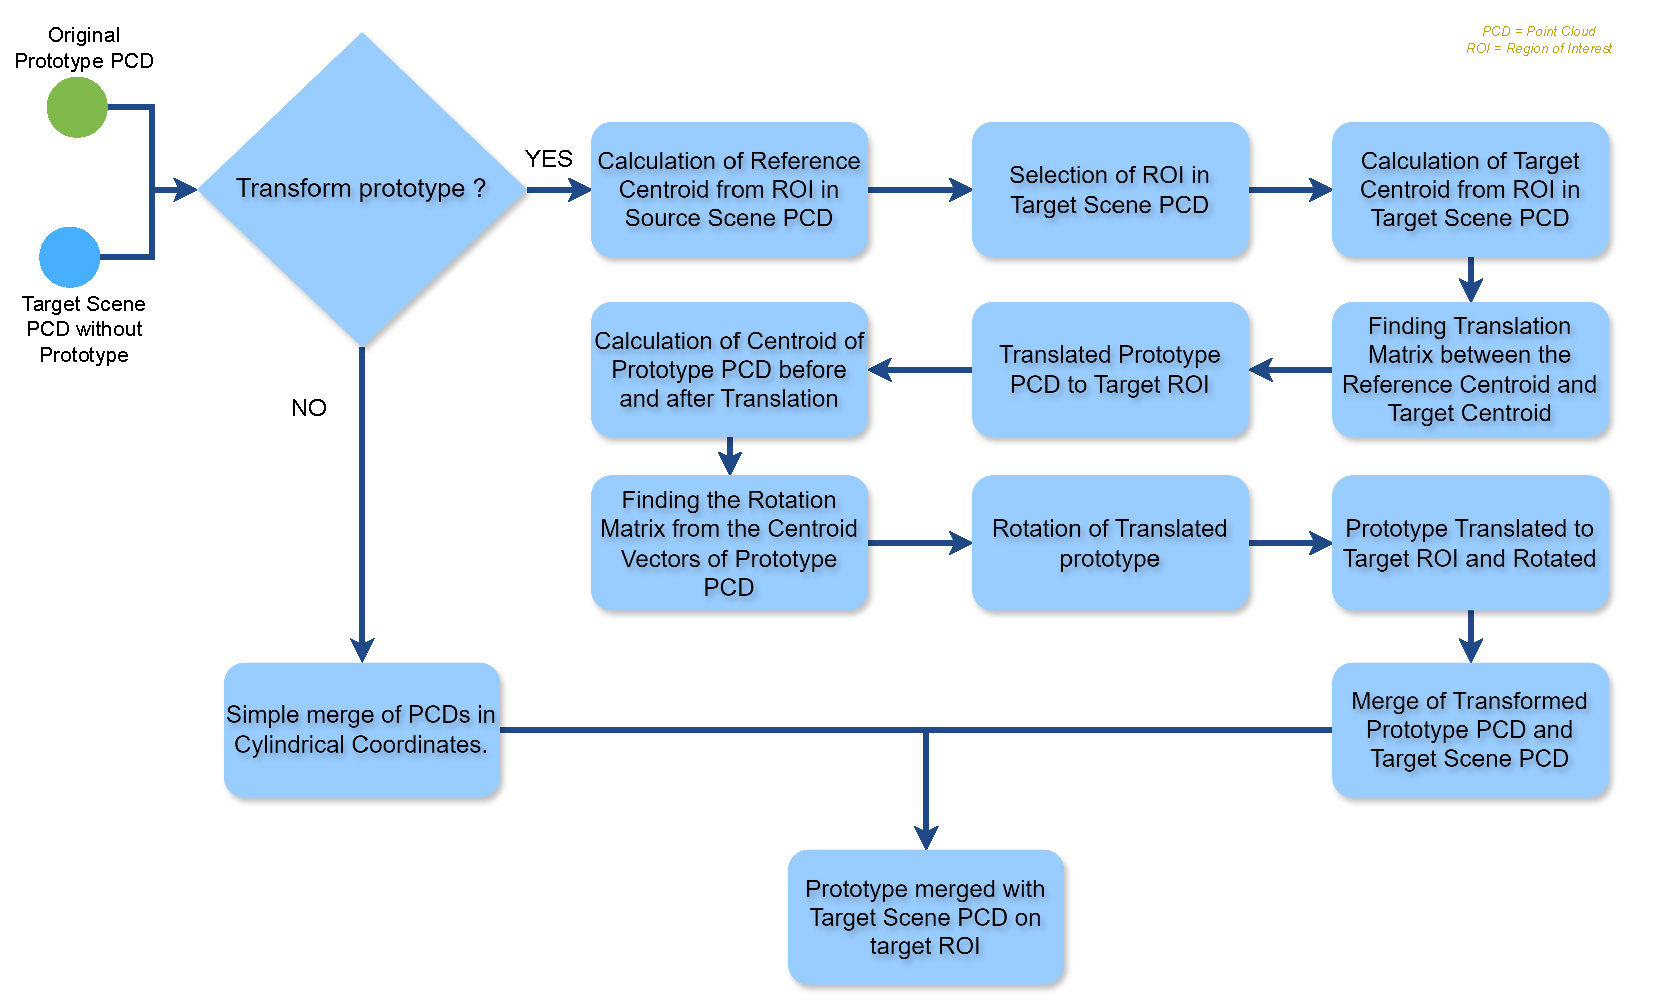
\includegraphics[width=1\linewidth]{97_graphics/concepts/prototype_extraction.pdf}
    \caption{Flowchart for the Transformation of Prototype \acrshort{pcd} to Target \acrshort{roi} and Merged with Target Scene \acrshort{pcd}}
    \label{fig:prototype_transform_and_merge}
\end{figure}

A simple geometrical approach is used for the transformation of the prototype to a region on the target scene cloud. If the prototype does not need to be transformed then it could be directly merged with the target scene and proceed with the next step. If the prototype needs to be transformed to a different location then first the centroid of reference is calculated from the region selected on the source scene cloud. This is calculated by adding all the points lying on the selected region on the source scene cloud that does not contain points from the prototype cloud. The resulting sum is divided via the overall count of considered points to get the average value of the x, y, and z axis or the centroid of the ground plane. This calculation helps to get the orientation of the ground plane in the selected region of interest where the prototype is situated. Since the reference centroid is calculated from the points in the region of interest but excluding the prototype points, when performing this step, one needs to be careful so that no prototype points or high z-values points are considered for centroid calculation. Under such circumstances, the resulting centroid may not accurately represent the ground plane. Such a situation could lead to errors in the transformation process, potentially causing the prototype to be positioned above the ground plane in the designated region of the target scene cloud.

After the calculation of the reference centroid, a desired region of interest is selected on the target location, and the target centroid is calculated for the selected region. Using the two centroids, a translation matrix is created with which the prototype is translated to the target region in the target scene cloud. Using the vectors representing the reference centroid and target centroid, from equation \ref{eq:angle_between_vectors} the rotation matrix is calculated.

\begin{figure}[htb]
    \centering
    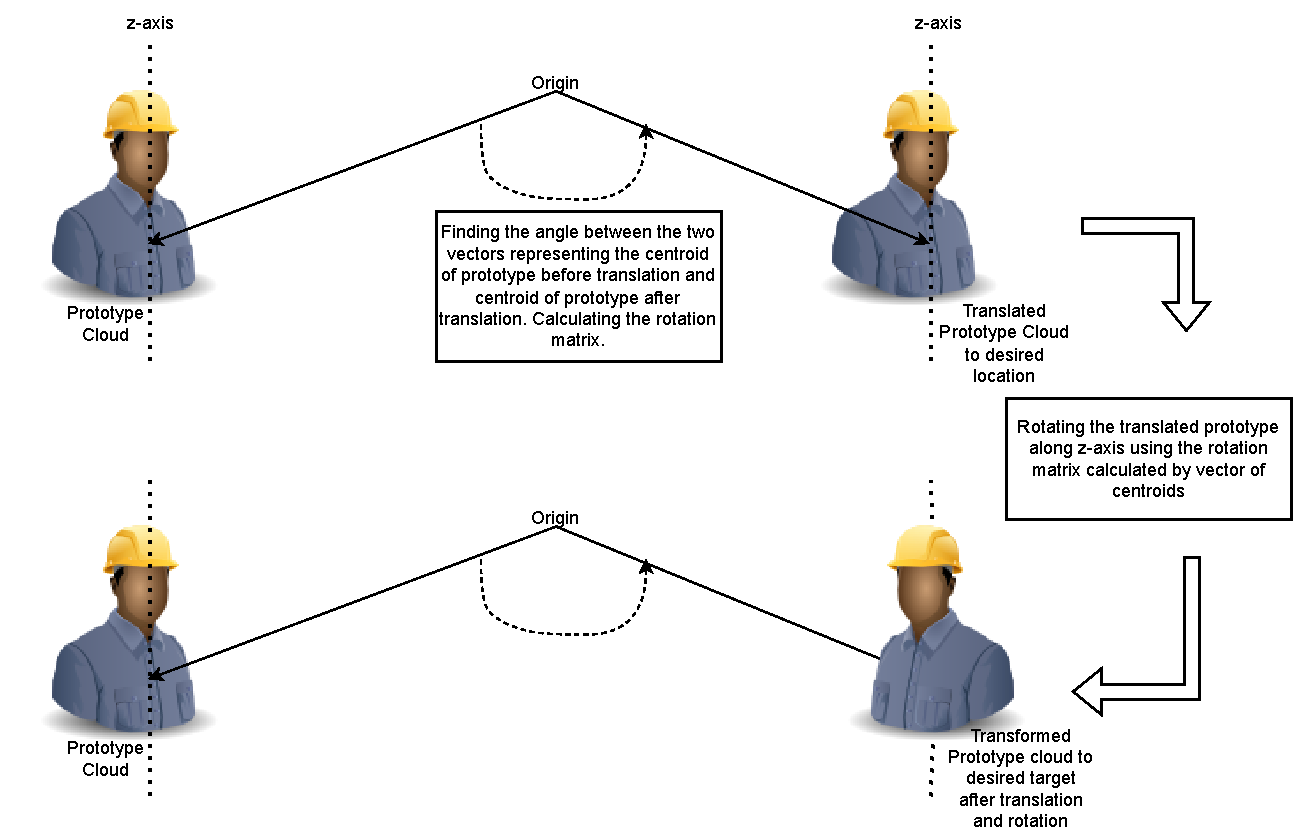
\includegraphics[width=0.8\linewidth]{97_graphics/concepts/rotational_matrix_calculation.pdf}
    \caption{Translation of Prototype, Calculation of Rotation Matrix and Rotation of Translated Prototype.}
    \label{fig:rotation_matrix_calculation}
\end{figure}

As shown in figure \ref{fig:rotation_matrix_calculation}, the calculated rotation matrix is then used to rotate the translated prototype cloud along the z-axis so that the transformed prototype object faces the origin. This is among the severely crucial actions. If the prototype is only translated to a desired location then the prototype might be facing in an incorrect direction (i.e. not viewing towards the origin). This false orientation of the prototype point cloud would result in a false calculation of points in the further steps as no points exist for surfaces that do not face the origin.

The transformed prototype cloud is then merged with the target scene cloud. The result is a prototype point cloud lying on top of the target region in the target scene cloud.


\subsection{Reconstruction of Prototype Point Cloud on Target Scene PCD based on distance from the Origin by Raycasting}

After the prototype point cloud has been placed in a target position on the target scene cloud, we need to find new point clouds of the prototype that accurately represent the prototype. We need to consider the following points for the reconstruction of points for the "transformed" prototype cloud.
\begin{itemize}
    \item Number of point cloud points for the prototype should vary based on distance from the origin.
    \item Need to consider the sparsity of prototype \acrshort{pcd} points based on distance from the origin.
    \item New points representing the prototype surface should accurately represent the surface.
    \item Recalculated points should not be random. It should be a collection of points that follow the laser rays that originate from the origin in the target scene cloud.
\end{itemize}

In raycasting, a series of rays, originating from a viewpoint is passed to a certain distance. The point of intersection of rays to the obstacle is noticed. Based on the distance from the obstacle point, a 3D perspective is reconstructed in a 2D map for the viewpoint. Similar to such a principle, we cast rays to the target scene that contains the "transformed" prototype point cloud. But before the emission of rays, we reconstructed the surface of the "transformed" prototype cloud. We have options such as alpha shapes, ball pivoting, and poisson surface reconstructions that are used for the reconstruction of the surface from the point cloud. The poisson surface reconstruction method, as outlined by \parencite{kazhdan2006poisson}, tackles the task of generating a smooth surface by addressing a regularized optimization problem. This approach contrasts with other methods that may yield less refined results, as they directly use the original points of the point cloud as the vertices of the resulting triangle mesh without any adjustments. Such reason leads us to use the poisson surface reconstruction for better construction of the surfaces. The Poisson surface reconstruction method extends its surface generation process to regions with sparse point density and even extrapolates into certain areas to create triangle meshes. The created triangle meshes also represent surfaces where there are minimum to no densities of points. To tackle such an issue, the reconstructed surface mesh is filtered. Filtering based on the density of the point also works but it requires manual setting of the threshold value. Instead of filtering by the density threshold value, triangles whose vertex do not contain the original point cloud points are removed. Following the later approach, no manual adjustment of the density threshold value is required.
After the surface mesh is filtered out and the resulting surface represents the mesh more accurately, rays are projected from the origin to a target region on the target cloud scene through the prototype surface mesh. To make the calculations faster, we select a region on the target scene cloud.

\begin{figure}[htbp]
    \centering
    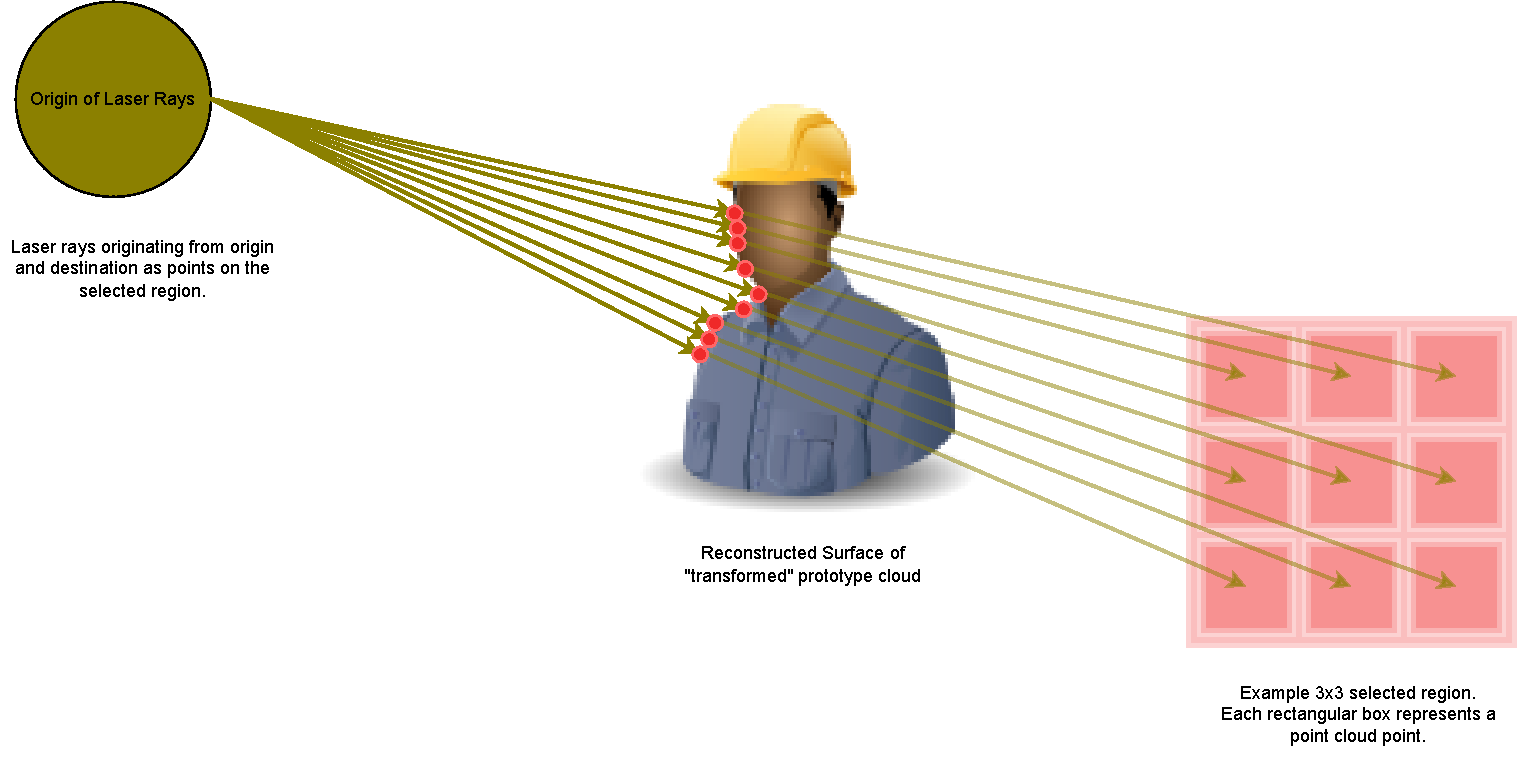
\includegraphics[width=1\linewidth]{97_graphics/concepts/raycasting.pdf}
    \caption{Rays traversing from the origin and terminating towards the selected points. Rays intersect with the reconstructed surface of the prototype, which is represented by red points}
    \label{fig:raycasting}
\end{figure}

As shown in figure \ref{fig:raycasting}, rays start from the origin and terminate at the selected region of interest. 3x3 rectangular box represents an example region that is selected on the target scene cloud. The region is selected in the target scene such that rays traversing from the origin to the designated points intersect the surface of the prototype(reconstructed surface of the Prototype).
Each 9 red box inside the selected region represents a point cloud. Thus in the example in figure \ref{fig:raycasting}, we are representing 9 points of a part of the selected target scene cloud. The rays travel toward the destination and some of the rays intersect the triangular mesh/surface of the prototype. Intersected point is calculated between the reconstructed surface mesh of the prototype and the casted rays. This intersected point gives us the new point cloud of the prototype. We call this new point cloud as Raycasted point cloud of prototype. This is represented by red points on the figure \ref{fig:raycasting}.

Two methods are explored for the calculation of the raycasted point cloud of the prototype. Since the reconstructed surface is represented by triangle mesh, when a single "laser beam" hits the surface of the prototype, it intersects with triangle in the triangle mesh. 

\subsubsection{Calculation of Point based on Centroid of Triangle}

Figure \ref{fig:concept-raycasting_single_triangle_by_centroid} demonstrates a single ray originating from the origin and terminating at a point in the selected region of interest in the target scene cloud. The ray intersects the triangle mesh at \((x, y, z)\). The vertex of the triangle is represented by \((x0, y0, z0)\), \((x1, y1, z1)\) and \((x2, y2, z2)\). To calculate the point \((x_c, y_c, z_c)\), we compute the centroid of the triangle mesh using equation \ref{equ:centroid_of_triangle}. These calculated points give us the raycasted point coordinates. This is represented by the red colored point in figure \ref{fig:concept-raycasting_single_triangle_by_centroid}. It can be viewed that the centroid of the point is not always the point of intersection. Here in the figure, the green point \((x, y, z)\) is the point of intersection to the triangle but this approach gives us the red color point \((x_c, y_c, z_c)\). To reduce the errors, other methods are experimented with.

\begin{figure}[htbp]
    \centering
    \begin{minipage}[b]{0.47\textwidth}
    \centering
    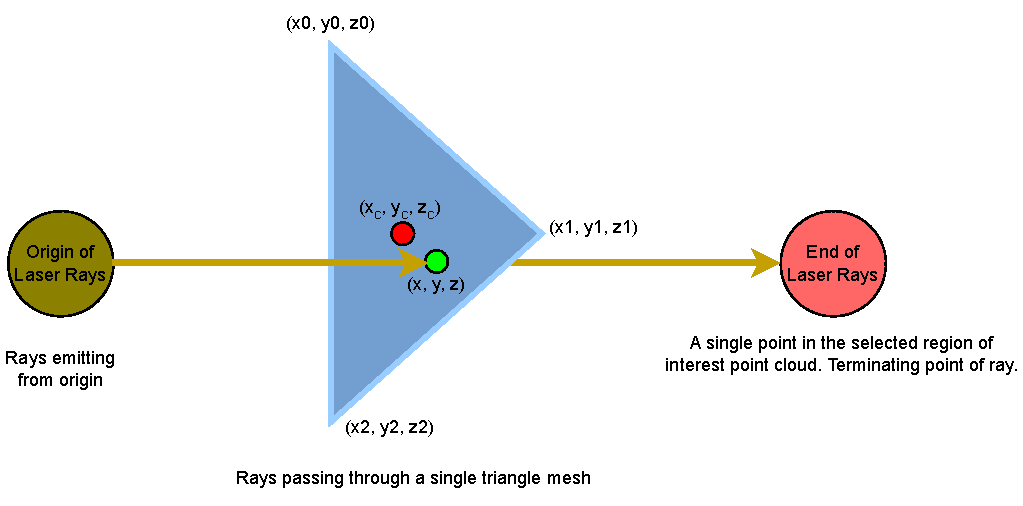
\includegraphics[width=1\linewidth]{97_graphics/concepts/raycasting_single_triangle_by_centroid.pdf}
    \caption{Calculation based on Centroid of the triangle.}
    \label{fig:concept-raycasting_single_triangle_by_centroid}
    \end{minipage}
    \hfill
    \begin{minipage}[b]{0.47\textwidth}
    \centering
    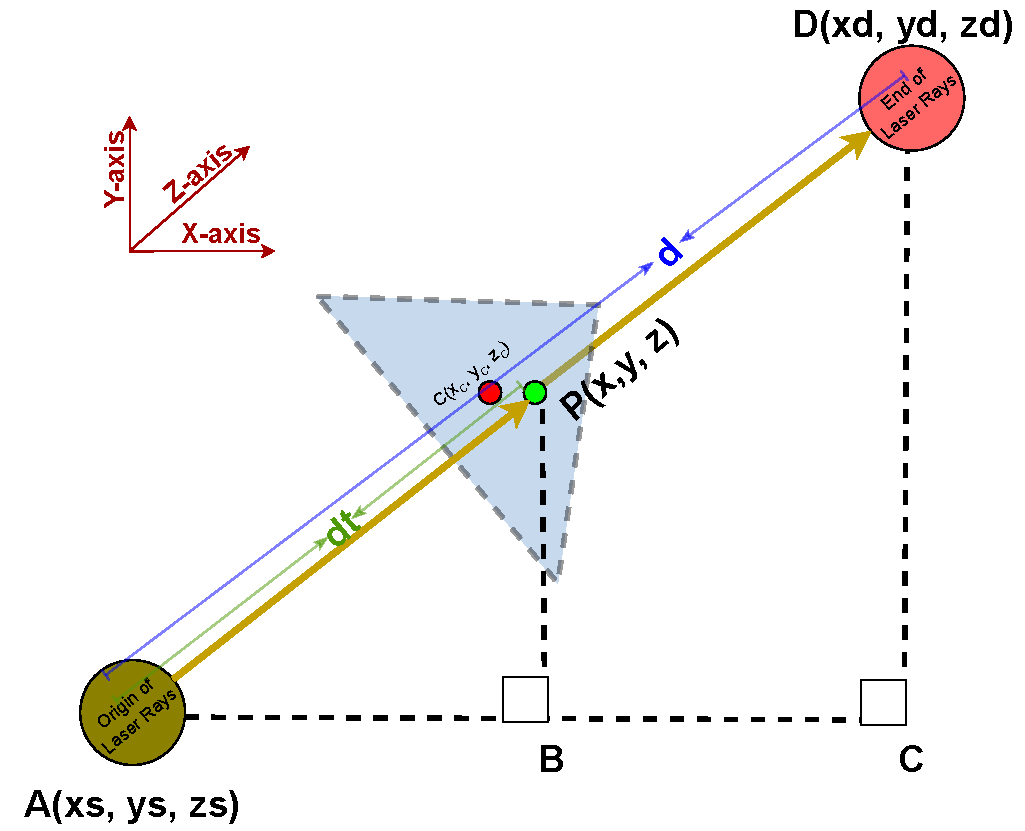
\includegraphics[width=1\linewidth]{97_graphics/concepts/raycasting_single_triangle_by_t_hit.pdf}
    \caption{Calculation based on hit distance to the triangle.}
    \label{fig:concept-raycasting_single_triangle_by_t_hit}
    \end{minipage}
\end{figure}

\subsubsection{Calculation of Point based on hit distance to the Triangle Mesh}
Using the centroid method to find the raycasted point is not always correct. The accuracy of the centroid method would depend on the proportion of triangles in the triangle mesh. The larger size of the triangle in the triangle mesh would result in a higher error rate. To eliminate such dependencies and error rates, the distance-based method is approached.  
In the figure \ref{fig:concept-raycasting_single_triangle_by_t_hit}, right-angle triangles are constructed. $\triangle ABP$ represents the smaller triangle. $\triangle ACD$ represents the larger triangle. \(dt\) represents the hit distance from the origin to the surface of the triangle. \(d\) represents the distance between the origin and the terminating point of the laser ray. Since two triangles are similar, using the law of similarity in triangles, we can write as follows : 

\begin{gather*}
\begin{aligned}
&\frac{AB}{AC} = \frac{AP}{AD} && \text{(Ratio of sides of triangle)}\hfill \\ \\
&\frac{x}{x_d} = \frac{d_t}{d} && \text{(Inserting length of the sides)}\hfill \\  \\
&x = x_d \times \frac{d_t}{d} && \text{(Result after Cross multiplication)}\hfill  \\  \\
\end{aligned}
\end{gather*}

\(X-axis\), \(Y-axis\), and \(Z-axis\) coordinates of the green color point can be obtained using the same approach.

\begin{equation}\label{eq:find_xyz}
    P(x, y, z) = \left( \: x_d \times \frac{d_t}{d}, \: y_d \times \frac{d_t}{d}, \: z_d \times \frac{d_t}{d} \: \right)
\end{equation}

\begin{equation}\label{eq:distance}
\text{distance(d)} = \sqrt{{(x_d - x_s)}^2 + {(y_d - y_s)}^2 + {(z_d - z_s)}^2}
\end{equation}

Equation \ref{eq:distance} represents the Euclidean distance between the two points in space (i.e. distance between vertex A and vertex D in figure \ref{fig:concept-raycasting_single_triangle_by_t_hit}). The \(d_t\) distance from the origin to the triangle can be obtained by raycasting. Hence, by using the equation \ref{eq:find_xyz}, the coordinates of point \(P(x,y,z)\) can be calculated. This is represented by the green color point in figure \ref{fig:concept-raycasting_single_triangle_by_t_hit}. As shown in the figure, this point accurately represents the intersected point of the "laser ray" with a triangle mesh. For the calculation of the raycasted point cloud of the prototype, this approach is followed. As a final result, the raycasted point can be obtained which is represented by the red colored points in figure \ref{fig:raycasting}.

\subsection{Shadowcasting on the Target Scene PCD by Raycasted Prototype Point Cloud}

After the points of the prototype \acrshort{pcd} are recalculated based on the distance and orientation from the origin, we call the points raycasted \acrshort{pcd} of the prototype. In the shadowcasting step, we reconstruct the shadow projected by the raycasted prototype on the target scene. Two methods for the calculation of shadow casting are experimented with. Two methods are the Hidden Point Removal (HPR) algorithm and calculation based on the Raycasted Rays.

\subsubsection{Approach using HPR algorithm}
Based on a certain viewpoint in a point cloud, the HPR algorithm tells us if a point in the point cloud is hidden or visible. Consider an example as shown in figure \ref{fig:shadow_casting}. In the figure, the left image of Armadilos is shown without applying the HPR algorithm. The right image is shown after applying the HPR algorithm. In the figure \ref{fig:shadow_casting}, we could not distinguish if the left image of Armadilos is facing backward or frontwards (toward the direction of the reader). Since all the points are practically visible, the left image of the Armadillos in the figure seems to be facing backward and frontwards at the same time, creating confusion. After applying the HPR algorithm, the output is represented by the right side of the image in figure \ref{fig:shadow_casting}. We can clearly say that the Armadilo is facing backward with its back towards the reader. On applying the HPR, for the figure \ref{fig:shadow_casting}, the viewpoint is selected to be a point in the direction of the reader or outwards from the screen. This resulted in points being removed that are hidden from the viewpoint.

\begin{figure}[htbp]
    \centering
    \begin{minipage}[b]{0.45\textwidth}
    \centering
    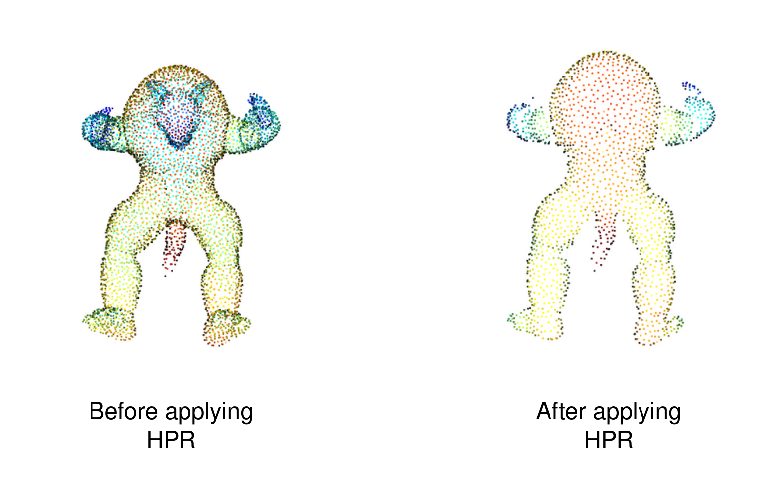
\includegraphics[width=0.5\linewidth]{97_graphics/concepts/shadowcasting_from_paper.pdf}
    \caption{Point cloud of Armadilos \parencite{open3d}}
    \label{fig:shadow_casting}
    \end{minipage}
    \hfill
    \begin{minipage}[b]{0.45\textwidth}
    \centering
    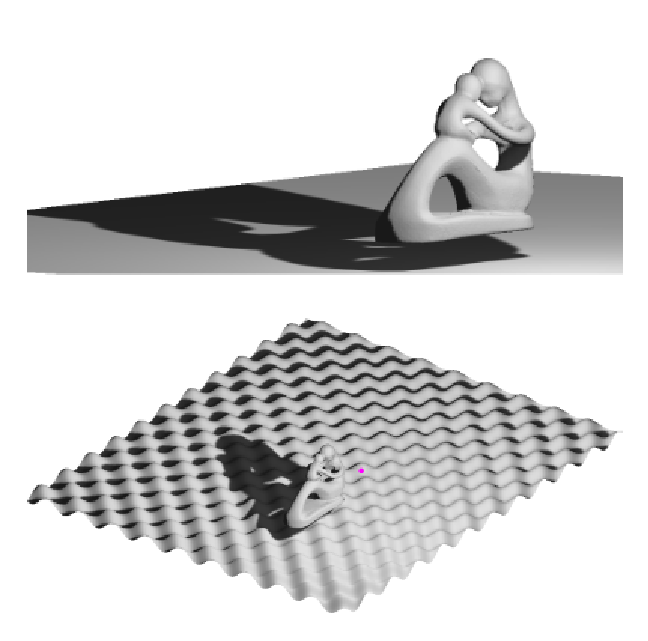
\includegraphics[width=0.5\linewidth]{97_graphics/concepts/hpr_reference_output.pdf}
    \caption{Shadow casting by HPR \parencite{katz2007}}
    \label{fig:hpr_reference_output}
    \end{minipage}
\end{figure}

In figure \ref{fig:hpr_reference_output}, the shadow is projected based on the visibility of points from the viewpoint. The viewpoint is defined by a pink color point on the bottom image of figure \ref{fig:hpr_reference_output}. Based on the visibility of the points from the viewpoint, the points are assigned low-intensity values or left unchanged. This resulted in the projection of shadow on the surface.
A similar principle is experimented for the casting of shadow by the raycasted point cloud on the target scene cloud. The viewpoint for HPR is set to the origin of the target scene point cloud. Instead of changing the intensity values of the hidden points, the points are removed from the point cloud and as a result, shadow-projected by the raycasted prototype on the target scene is acquired as output. 

\begin{figure}[htbp]
    \centering
    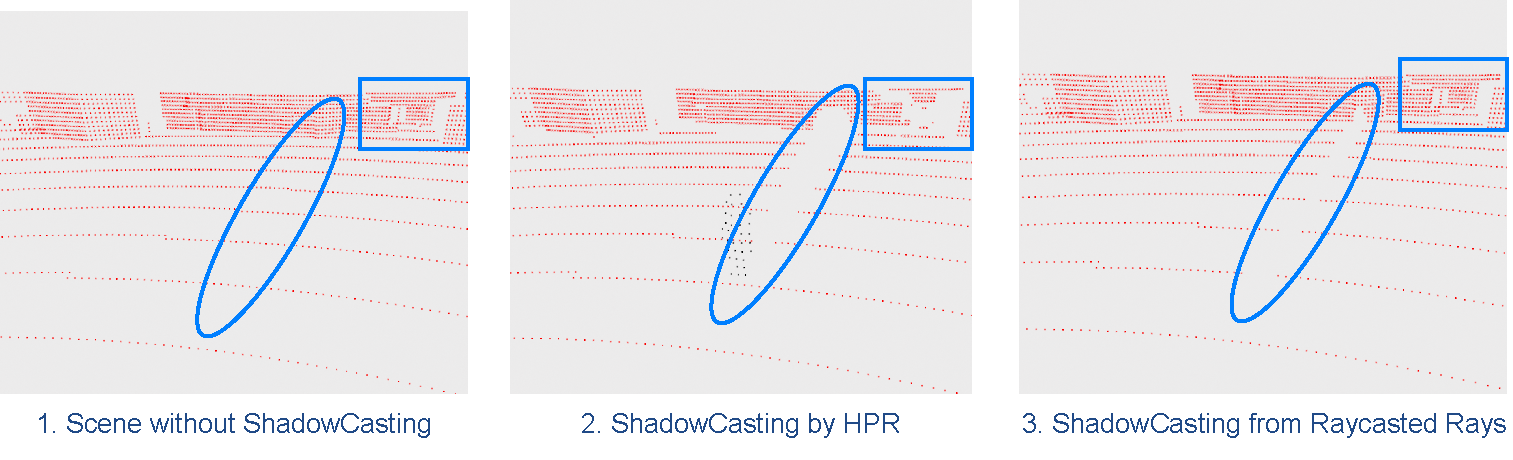
\includegraphics[width=0.9\linewidth]{97_graphics/concepts/shadow_casting_difference.pdf}
    \caption{Shadow Casting Difference between two methods}
    \label{fig:concept-shadow_casting_difference}
\end{figure}


\subsubsection{Approach using Raycasted Rays}
This approach is simple yet very effective. Instead of using the HPR algorithm for the calculation of shadow projection on the scene, the ray casted rays are considered for further calculations. Rays originate from the origin of the target scene point cloud and terminate at the points on the ROI in target scene cloud. Any rays intersecting the surface of the prototype give the raycasted point. Rays intersecting with the prototype surface means that the terminating point of the ray will be hidden by the surface of the prototype. Some rays do not intersect with the surface of the prototype. The terminating points of such rays are not hidden by the surface of the prototype. As a result, an accurate shadow of the prototype surface can be calculated. As shown in figure \ref{fig:concept-shadow_casting_difference}, this approach gives a perfect shadow of the reconstructed prototype surface. The blue rectangular box in the figure shows that applying the HPR algorithm affected the points that were not in the shadow region of the raycasted prototype. However, points not lying in the shadow region of the prototype were not affected using the raycasted method for shadow calculation. This approach is implemented for shadow calculation.
\begin{figure}[htbp]
    \centering
    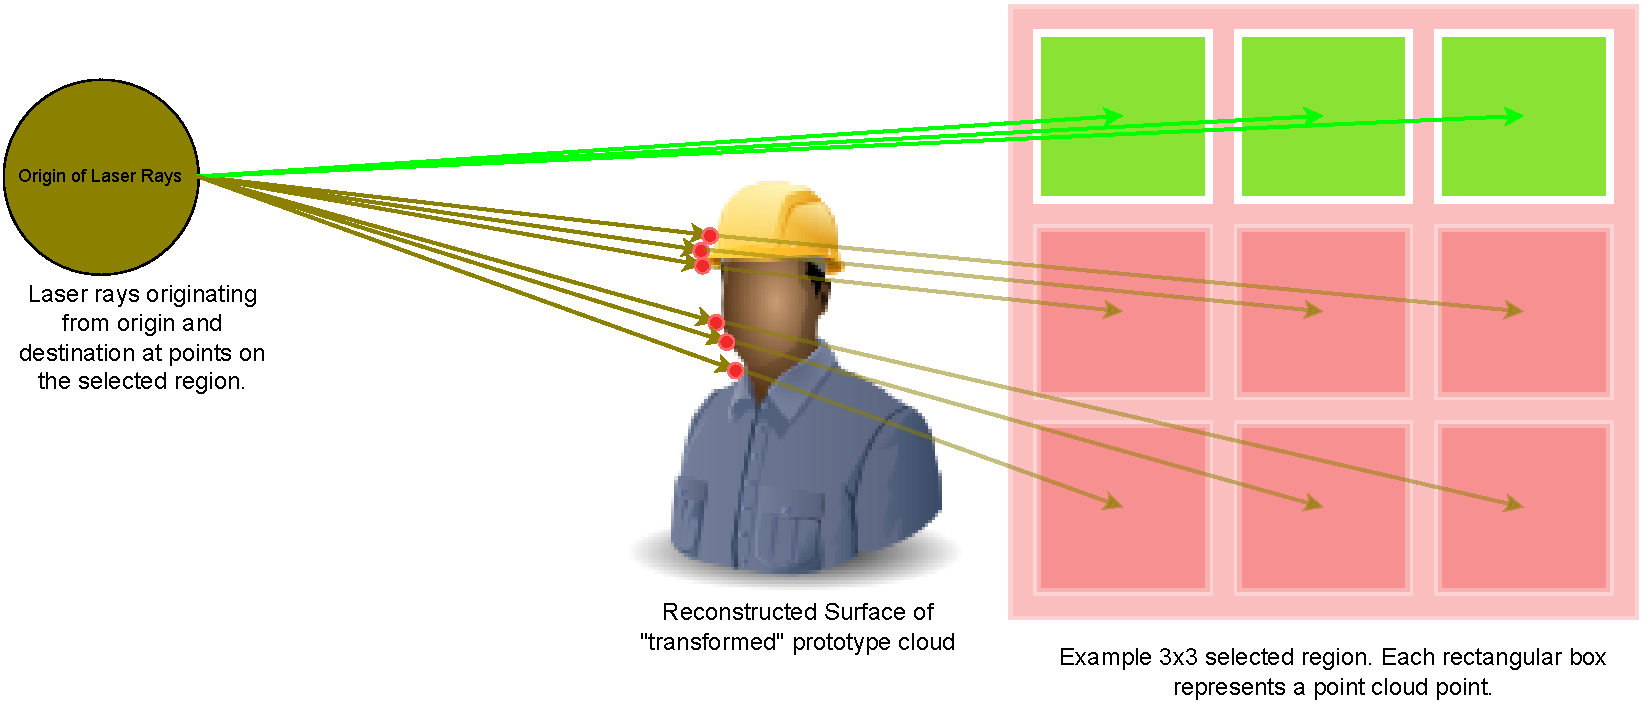
\includegraphics[width=0.9\linewidth]{97_graphics/concepts/shadow_casting_by_raycast_method.pdf}
    \caption{Shadow Casting Approach using Raycasted Rays}
    \label{fig:concept-shadow_casting_by_raycast_method}
\end{figure}

Figure \ref{fig:concept-shadow_casting_by_raycast_method} shows an example of shadow casting on the target \acrshort{roi} in target scene \acrshort{pcd}. The green-colored rays, originating from the origin to the point in the selected region, were not intersected with the reconstructed prototype surface(triangle mesh). So the terminating points of the green colored rays are not hidden from the origin. This is represented by the green-colored square on the figure. The red-colored square represents that the point is hidden by the surface. The rays that originate from the origin designated to the red-colored square are blocked by the surface of the prototype. The intersected point of the rays with the surface is represented by red-colored points and is called the raycasted points. The terminating point of the rays blocked by the surface or prototype is the shadowed region.

\section{Functional Description of the implementation}

Figure \ref{fig:functional_description_of_concept} shows an example of high-level implementation details of the project. The images present in the top row of the figure \ref{fig:functional_description_of_concept} represent scenes. The top left image represents a source scene. An Asset (Person) is present on the scene, which is represented in the red rectangular box. The top middle image of the figure represents a target scene. The goal of the project is to extract a person from the source scene and insert the extracted person into the target scene (without manipulating the objects in simulations or real-world). This results in a new scene. In the figure, the target scene is modified in such a way that a person is now present on the target scene. So the recombination between the two upper left scenes would result in a new scene similar to the top right of the figure \ref{fig:functional_description_of_concept}.
These different scenes were captured in the \acrfull{carla} simulator \parencite{Dosovitskiy17}. An ego vehicle was summoned on CARLA using carla-ros-bridge. The Asset or Person was summoned to a specified location near the ego vehicle.

\begin{figure}[htbp]
    \centering
    \includegraphics[width=1\linewidth]{97_graphics/concepts/functional_description_of_concept.pdf}
    \caption{Functional description of the implementation}
    \label{fig:functional_description_of_concept}
\end{figure}

\section{Technical Description of the implementation}
The aim of the project is the creation of a new scene. This project works on the point cloud level. Functional description of the projects shows a higher level overview of the project using images from \acrshort{carla}. This section describes the technical aspects of the project. The point cloud images shown on the top row in figure \ref{fig:technical_description_of_implementation} correspond to the point cloud of scenes represented by the top row images in figure \ref{fig:functional_description_of_concept}. The ego vehicle is attached with a lidar sensor, which gives a lidar point cloud of the current scene continuously. The point cloud data is made available to \acrfull{ros} topic by carla-ros-bridge, which is then captured by written scripts. 

\begin{figure}[htbp]
    \centering
    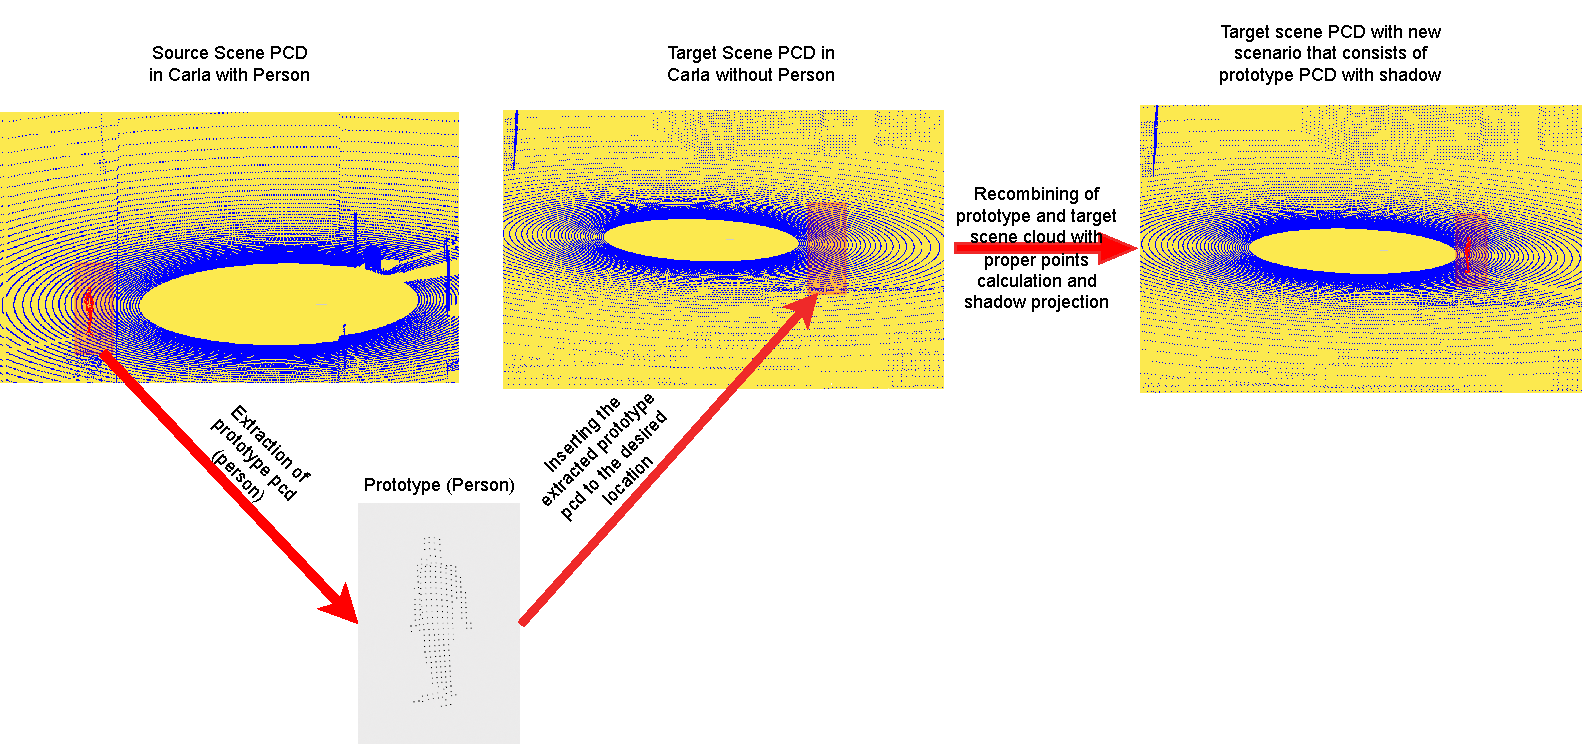
\includegraphics[width=1\linewidth]{97_graphics/concepts/technical_description_of_concept.pdf}
    \caption{Technical description of the implementation}
    \label{fig:technical_description_of_implementation}
\end{figure}

The image on the top row leftmost side in figure \ref{fig:technical_description_of_implementation} represents a source scene cloud. The task of the project is to extract the prototype cloud from the source scene cloud. The prototype cloud is represented by red colored points on the source scene cloud. The prototype point cloud is to be extracted using the geometric features of the point cloud. The region of interest from where we would like to extract and insert a prototype is represented by a red rectangular box in all the top row images in figure \ref{fig:technical_description_of_implementation}. In the source scene cloud, geometric features on the selected region of interest are calculated. The separation of the prototype point cloud from the target scene is done by thresholding the geometric features. This gives us an extracted prototype cloud represented by the image on the bottom row of figure \ref{fig:technical_description_of_implementation}. This prototype needs to be placed on the target scene region of interest in the top row middle image of the same figure. With the proper transformation of the prototype cloud according to the geometry of the target scene cloud, the prototype is placed and the projected shadow is calculated. A final output point cloud is created by combining the prototype from the source scene cloud into the target scene cloud. This new point cloud is represented by the top row rightmost image in the figure \ref{fig:technical_description_of_implementation}.

			\chapter{Prototypical Implementation of the Concept}
From the source scene point cloud, a prototype point cloud (person \acrshort{pcd}) is extracted. A region of interest (\acrshort{roi}) is defined in the source scene point cloud which contains the prototype point cloud. Geometric features are calculated for the selected region of interest. Non-prototype points are filtered out based on the geometric feature values of the points. Thus a prototype \acrshort{pcd} is obtained from the source scene \acrshort{pcd}. The acquired prototype point cloud is transformed into a target location on the target scene \acrshort{pcd}. The point cloud for the prototype is recalculated on the target scene \acrshort{pcd} based on the location of the prototype on the target scene \acrshort{pcd}. Surface reconstruction and Raycasting are used for the recalculation of points of the prototype point cloud. Thus obtained point cloud of the prototype after raycasting is termed as Raycasted Prototype \acrshort{pcd}. Shadow projected by the raycasted prototype point cloud on the target scene cloud is computed. Hence a new scenario of the target scene point cloud is created by the recombining of source scene \acrshort{pcd} and target scene \acrshort{pcd}. The following section explains each step in detail. For the purpose of the experiment, semantic-lidar data captured from \acrshort{carla} was used for both the source scene point cloud and target scene point cloud.

\section{Loading a Source Scene Point Cloud}
 In the figure \ref{fig:result-prototype_on_source_scene}, we can see points in the point cloud that are either black or green in color. To color the scene, we have used the ObjIdx value from the semantic-lidar data obtained from \acrshort{carla}. The semantic LIDAR data is sourced from CARLA to only facilitate the visualization of the prototype point cloud. The value of the ObjIdx is zero for stationery objects and the value of ObjIdx is non-zero for non-stationery objects. Based on this value, if the ObjIdx is zero for the point, the point is colored green and if the ObjIdx is non-zero then the point is colored black. In figure \ref{fig:result-prototype_on_source_scene}, we can see a prototype (person), located on the left part of the figure, represented by black in color. The point cloud in figure \ref{fig:result-prototype_on_source_scene} represents the \acrshort{carla} source scene as shown in functional implementation figure \ref{fig:functional_description_of_concept}.

\begin{figure}[htbp]
    \centering
    \begin{minipage}[b]{0.45\textwidth}
    \centering
    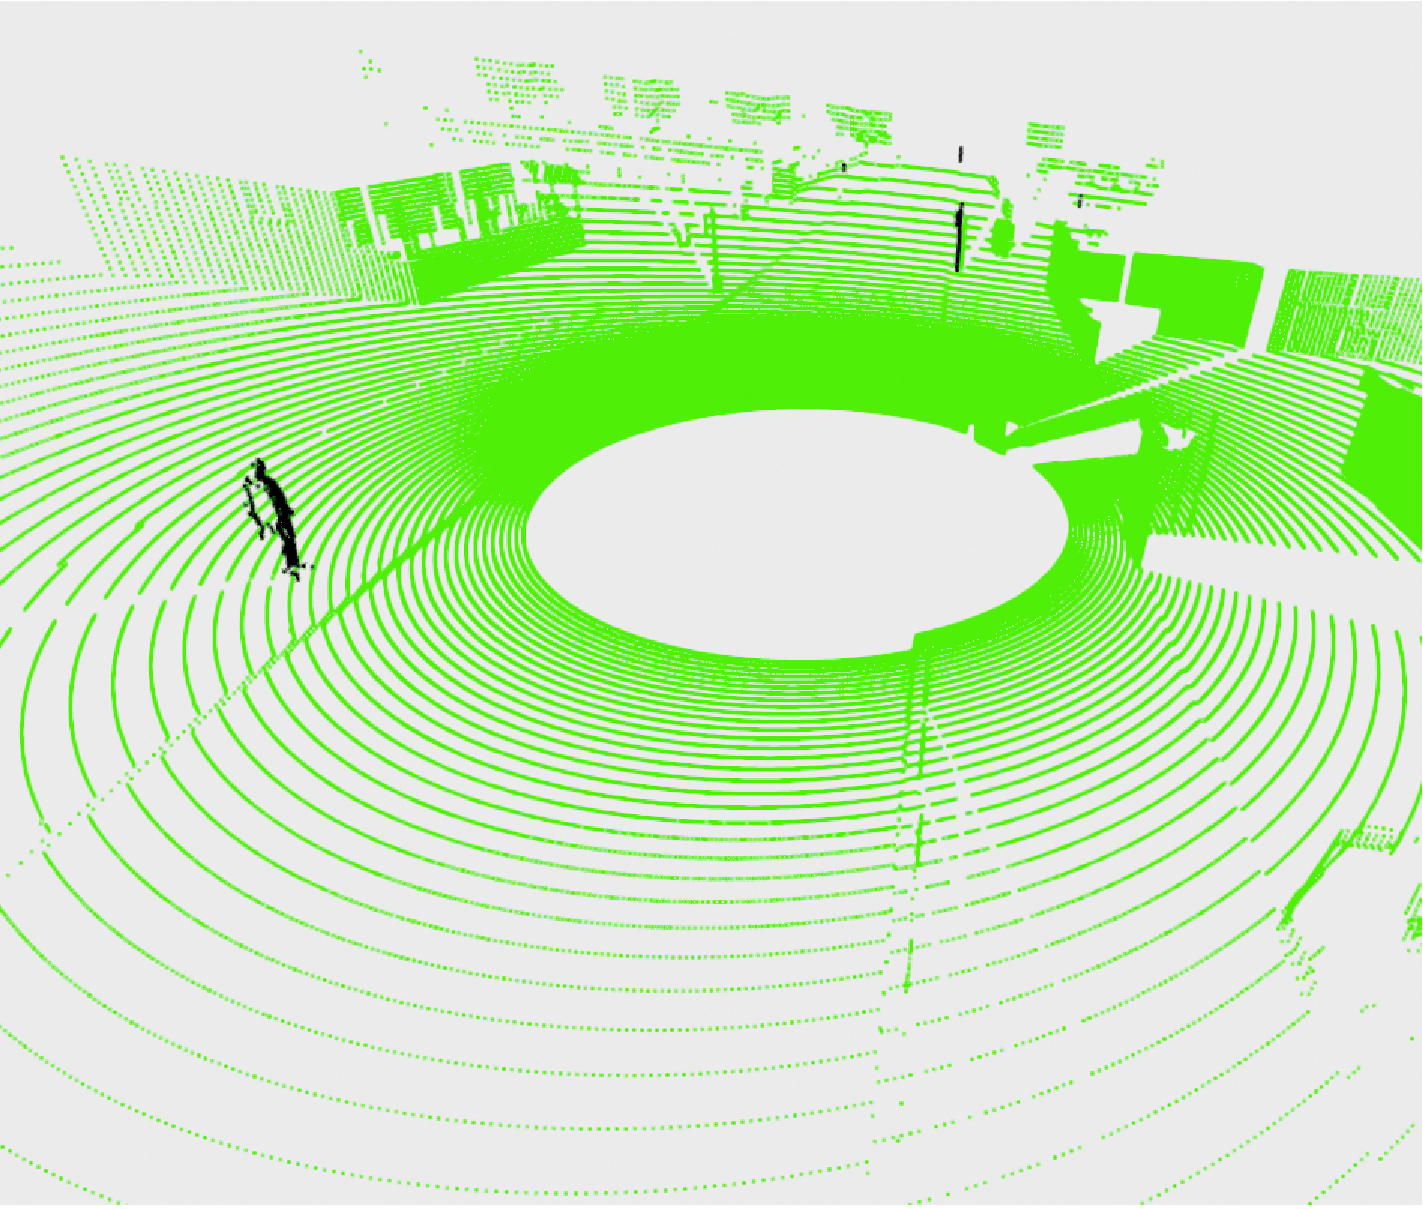
\includegraphics[width=1\linewidth]{97_graphics/results/prototype_on_source_scene_cloud.pdf}
    \caption{Prototype in Source Scene \acrshort{pcd}.}
    \label{fig:result-prototype_on_source_scene}
    \end{minipage}
    \hfill
    \begin{minipage}[b]{0.45\textwidth}
    \centering
    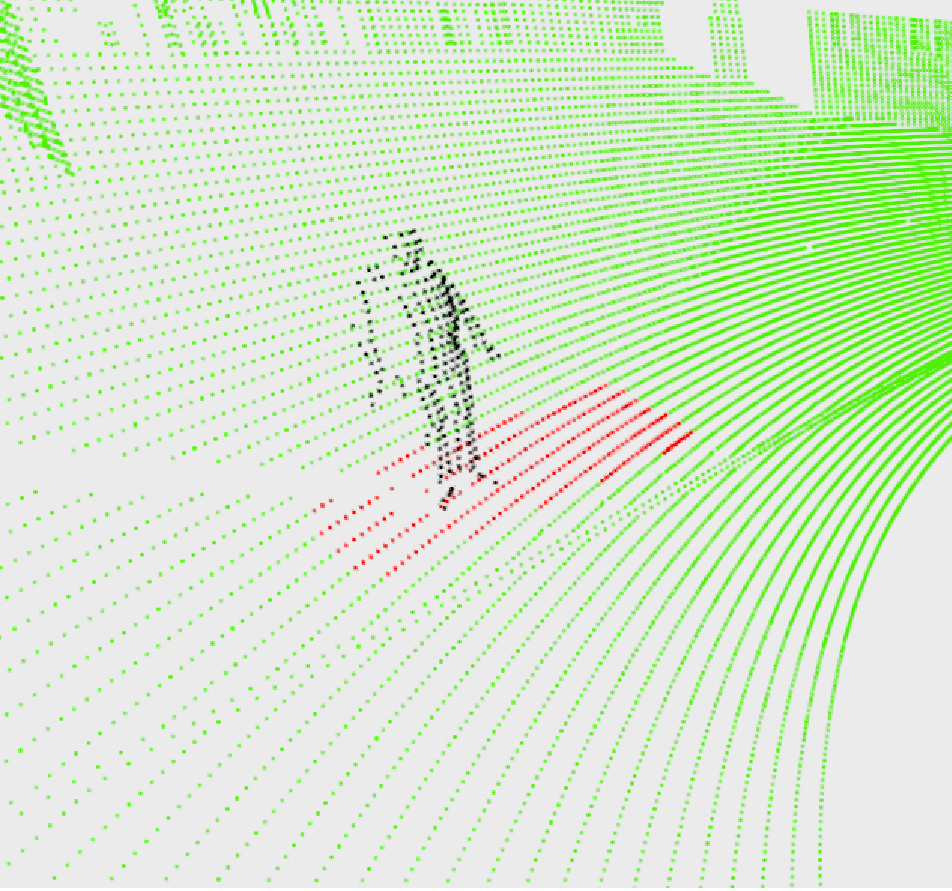
\includegraphics[width=1\linewidth]{97_graphics/results/roi_select_source_scene_cloud.pdf}
    \caption{Selection of \acrshort{roi} on Source Scene \acrshort{pcd}.}
    \label{fig:result-roi_select_source_scene}
    \end{minipage}
\end{figure}


\section{Selection of Region of Interest on Source Scene Point Cloud}
Since we plan on extracting the prototype from the source scene cloud, we need to specify the region on the source scene where we would like to extract the prototype \acrshort{pcd} from.

In figure \ref{fig:result-roi_select_source_scene}, the region of interest is represented by red-colored points plus any higher z-values points lying within the region. For ease of clarity, we have not changed the color of the prototype. First, a region is selected around the prototype manually. This is done manually by using the mouse cursor. At first, the position of the cursor is noted on the screen, if something is clicked on the screen then the relative position of the cursor on the world coordinates (the world where the point cloud is being visualized, the \acrshort{gui} for visualization) is calculated. Squared distances between the points on the point cloud and the world coordinate point are calculated. Based on minimum distance, a point on the point cloud is selected and marked with red color. Since manually selecting a list of points in a source scene cloud would take a lot of time, minimum x, minimum y, maximum x, and maximum y are calculated from the manually selected boundary region of interest. All the points that lie within the boundary value are finally selected as a region of interest on the source scene \acrshort{pcd}, from where a prototype \acrshort{pcd} is to be extracted.

\section{Extraction of Prototype from Source Scene Point Cloud}
Geometric features are calculated for the selected region of interest (\acrshort{roi}) from the source scene \acrshort{pcd}. Based on the number of nearest neighbors as 5 using "KDTreeSearchParamKNN" in open3d \parencite{open3d}, the nearest neighbor is searched for each point in the selected \acrshort{roi}. Using the kd-search tree, the covariance matrix and then the eigenvalue are computed after finding the local neighbors for each point in \acrshort{roi}. Utilizing the formulas for the calculation of geometric features as in equation \ref{eq:surf_var}, geometric features(surface variation) are calculated for each point in the \acrshort{roi} point cloud. The geometric feature values are filtered out by the appropriate threshold and finally, the remaining point having the valid geometric features in the selected \acrshort{roi} on the source scene \acrshort{pcd} is extracted, this extracted point cloud represents the prototype point cloud or original prototype point cloud.

\begin{figure}[htbp]
    \centering
    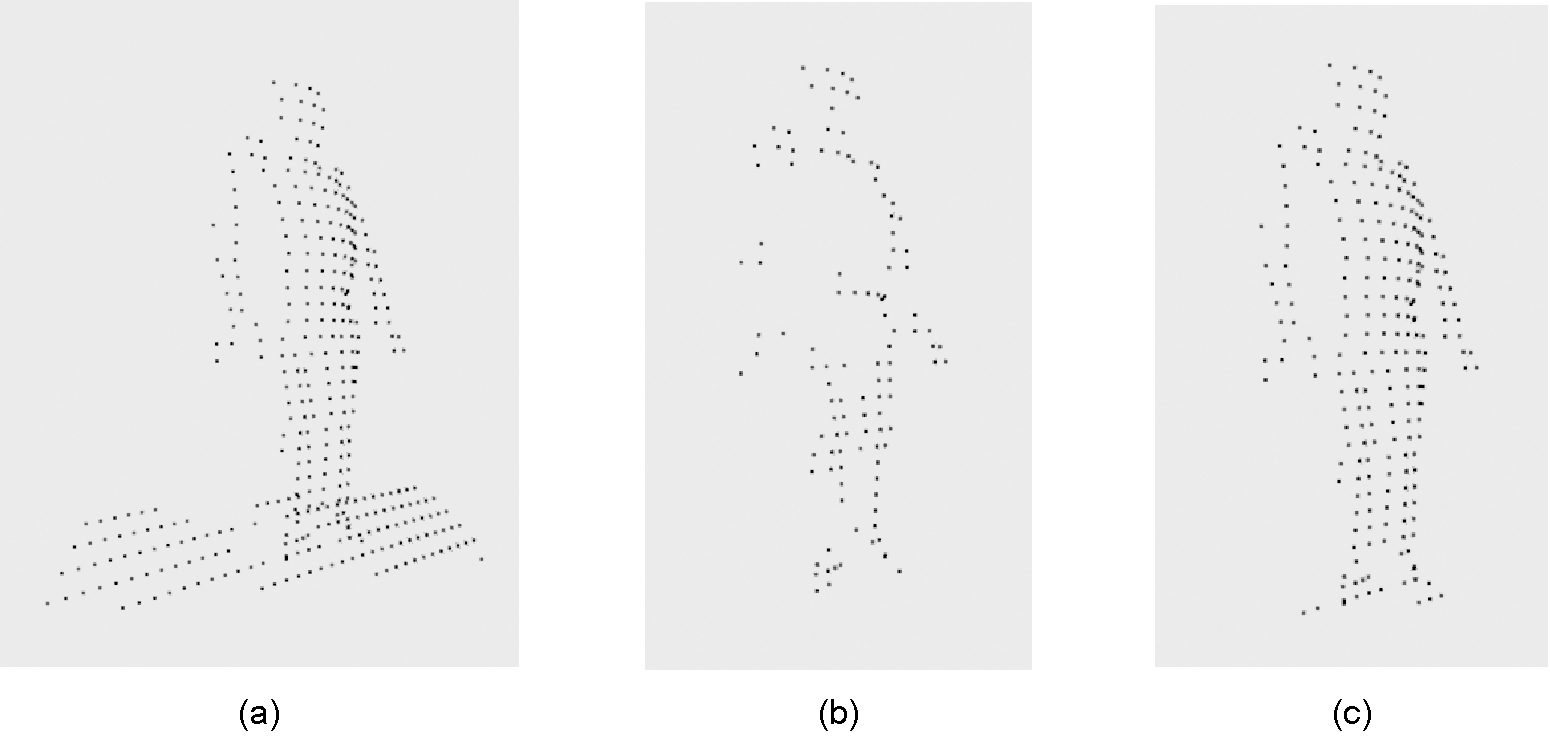
\includegraphics[width=0.8\linewidth]{97_graphics/results/prototype_extracted.pdf}
    \caption[Extracted Prototype Point Cloud from Source Scene \acrshort{pcd}.]{Extracted Prototype Point Cloud from Source Scene \acrshort{pcd} for different threshold of Surface Variation of points in selected \acrshort{roi} (a) \(Surface Variation \geq 0 \)  (b) \(Surface Variation \geq 0.05 \)  (c) \(Surface Variation \geq 10^{-8} \).}
    \label{fig:result-prototype_extracted}
\end{figure}

Trial and error were employed to explore different threshold values for surface variation, aiming to filter the prototype's point cloud optimally. As depicted in Figure \ref{fig:result-prototype_extracted}, a range of filtered point clouds for the prototype are displayed alongside their respective threshold values. Notably, the analysis reveals the utilization of a remarkably low threshold value \(10^{-8}\) for extracting the prototype's point cloud. This decision is attributed to the synthetic origin of the point cloud sourced from \acrshort{carla}, which lacks the randomness typically observed in the real-world LiDAR point clouds. The resulting point cloud obtained from this process is referred to as the "extracted prototype point cloud" or simply the "(original) prototype point cloud."

\section{Transformation of Prototype to a position on Target Scene Point Cloud}
The extracted prototype cloud could either be merged with the target scene \acrshort{pcd} on the original location (if the extracted prototype \acrshort{pcd} aligns properly with the target scene \acrshort{pcd}) or the prototype could also be transformed to a different location on the target scene \acrshort{pcd}.

\begin{figure}[htbp]
    \centering
    \begin{minipage}[b]{0.45\textwidth}
    \centering
    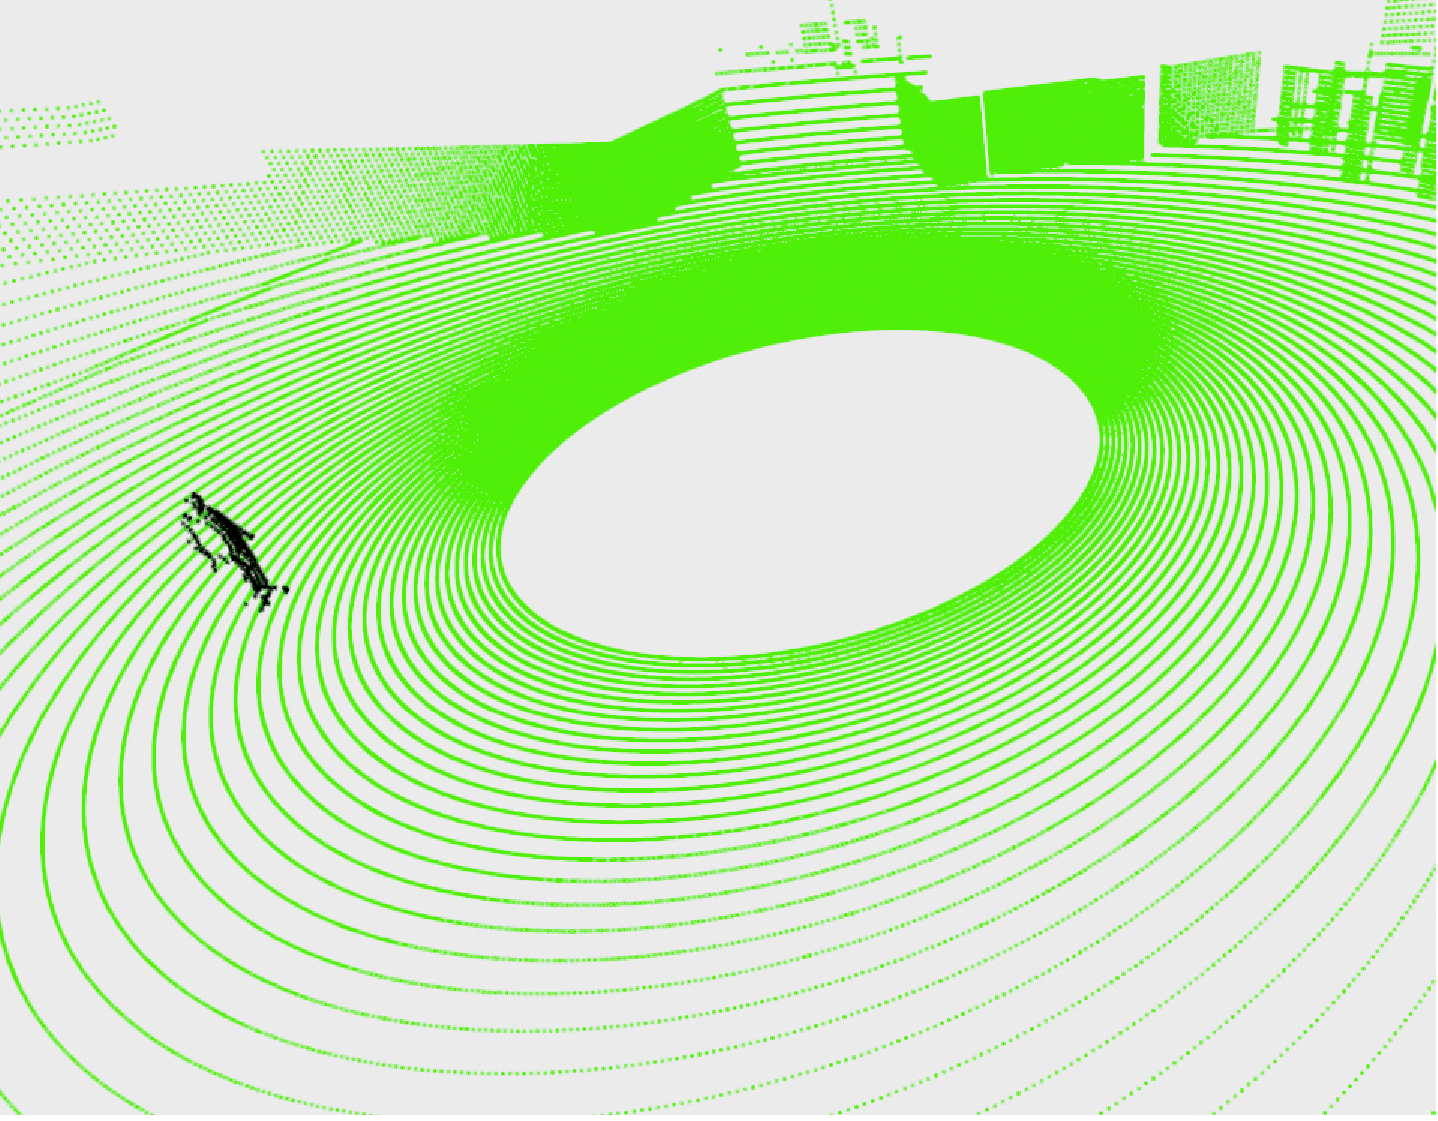
\includegraphics[width=1\linewidth]{97_graphics/results/prototype_on_target_scene_original_location.pdf}
    \caption{Prototype \acrshort{pcd} on Target Scene \acrshort{pcd} without transformation.}
    \label{fig:result-prototype_on_target_scene_original_location}
    \end{minipage}
    \hfill
    \begin{minipage}[b]{0.45\textwidth}
    \centering
    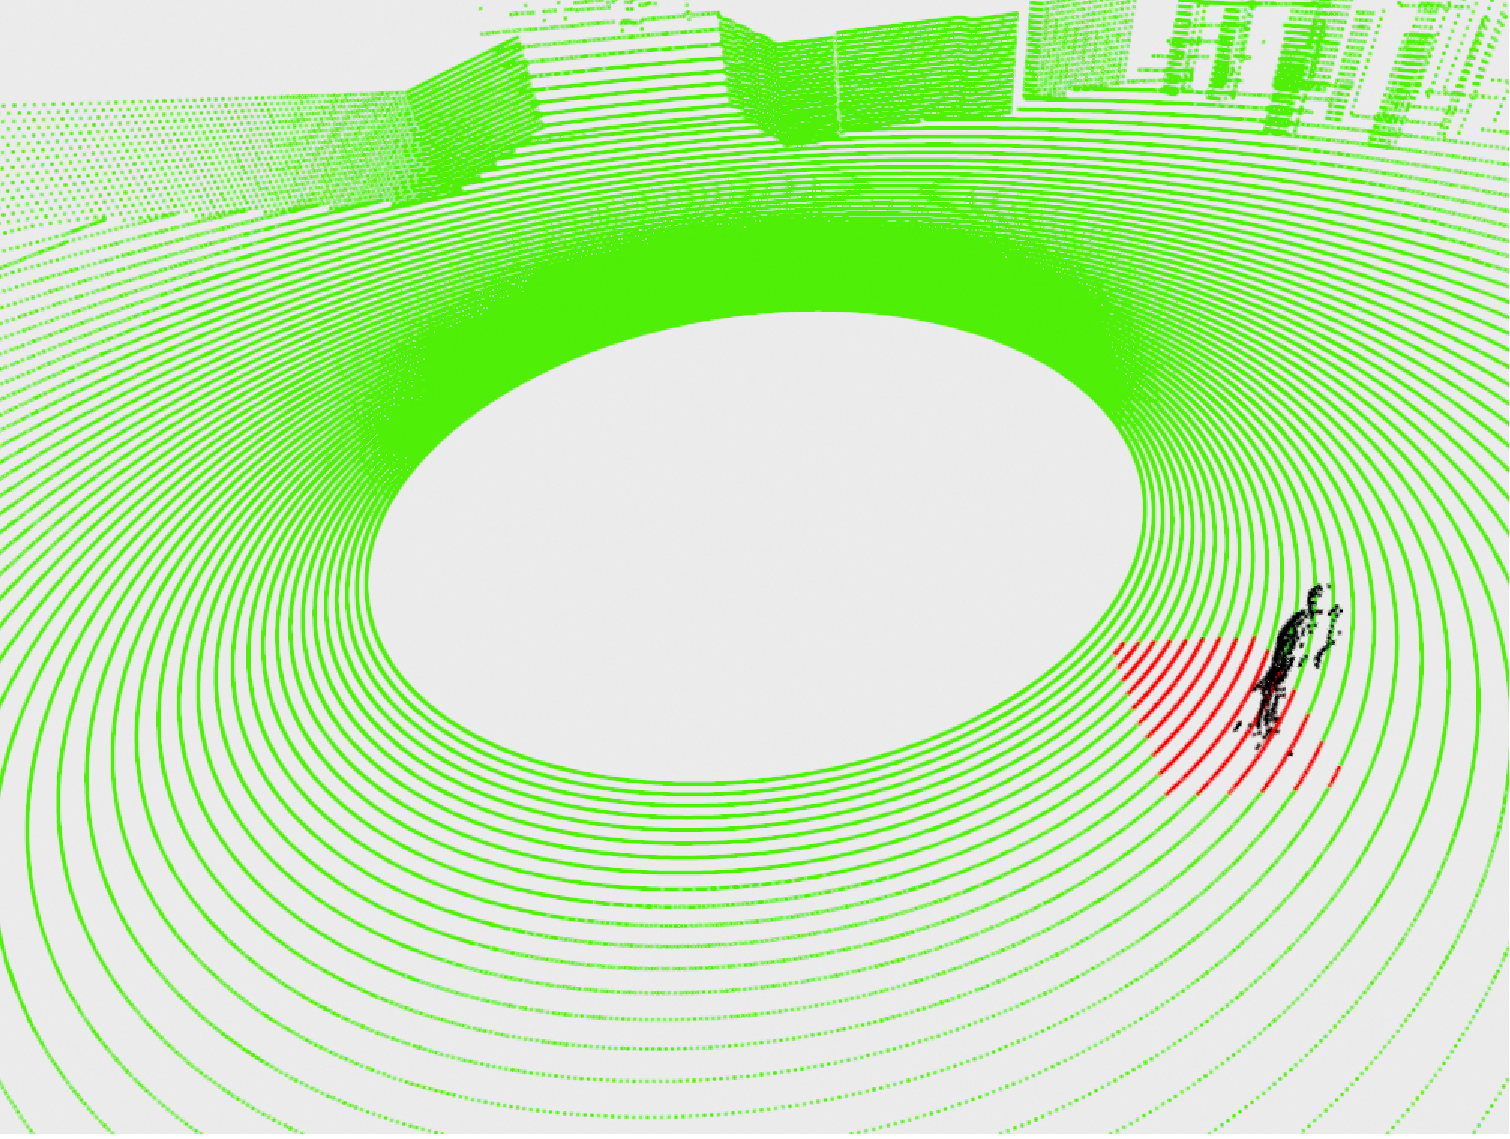
\includegraphics[width=1\linewidth]{97_graphics/results/prototype_on_target_scene_different_location.pdf}
    \caption{Prototype \acrshort{pcd} on Target Scene \acrshort{pcd} to a different position after transformation.}
    \label{fig:result-prototype_on_target_scene_different_location}
    \end{minipage}
\end{figure}

Figure \ref{fig:result-prototype_on_target_scene_original_location} shows a prototype \acrshort{pcd} (black points) without any transformation located on a target scene \acrshort{pcd}. Since the prototype is standing on top of the target scene and no irregularities were seen when concatenating the prototype point cloud (\acrshort{pcd})to the target scene point cloud (without transformation), we could also continue working with this position. Examples of irregularities encompass instances where a prototype appears submerged within the ground plane or traverses through a wall. If the prototype needs to be transformed to a different position, \acrfull{roi} is selected on the target scene point cloud. The selected ROI is shown by red colored points in figure \ref{fig:result-prototype_on_target_scene_different_location}. The translation and rotation matrix is calculated based on the reference centroid and target centroid as explained in figure \ref{fig:rotation_matrix_calculation}. One thing to note here is that when the position of the prototype is changed in figure \ref{fig:result-prototype_on_target_scene_different_location}, the prototype is also rotated according to the position change from the origin. Using the calculated rotational matrix, the prototype is rotated around the z-axis through the centroid of the prototype. This is an important step. Since we are not recalculating the side points or backside surfaces of a prototype, it is crucial to maintain the direction of the prototype relative to the origin. In our case, the prototype is still facing the origin.

\section{Surface Reconstruction and Filtering}
After the position of the prototype \acrshort{pcd} has been finalized on the target scene \acrshort{pcd}, the next step is the reconstruction of the surface. Using the Poisson reconstruction method, the surface of the prototype is reconstructed.

\begin{figure}[htbp]
    \centering
    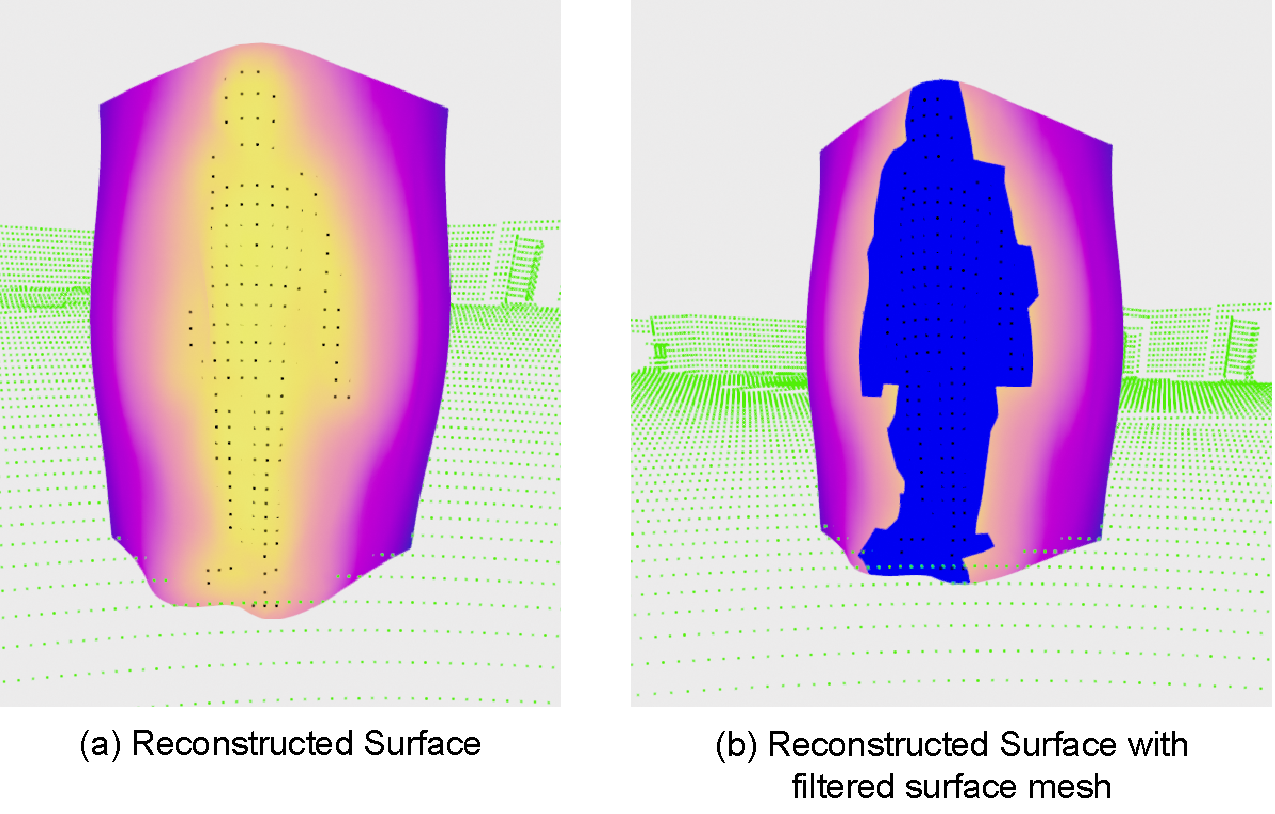
\includegraphics[width=1\linewidth]{97_graphics/results/surface_reconstruction.pdf}
    \caption[Reconstructed Surface of the Prototype on the Target Scene \acrshort{pcd}.]{Reconstructed Surface of the Prototype on the Target Scene \acrshort{pcd} (a) Reconstructed Surface with varying density of points (b) Reconstructed surface with filtered surface mesh (blue).}
    \label{fig:result-surface_reconstruction}
\end{figure}

Figure \ref{fig:result-surface_reconstruction} \((a)\) represents the total reconstructed surface visualized by varying density of points on the surface. The yellow color surface represents the region with a higher point density. The purple-colored surface in the figure represents the region with lower point density. The reconstructed surface of the prototype represents a triangle mesh. Since the prototype is relatively smaller than the reconstructed surface as shown in figure \ref{fig:result-surface_reconstruction} \((a)\), we need to filter the undesired surface of the reconstructed prototype. Using density value for filtering also works but requires lots of trial and error to get an optimal value, so we filtered the undesired reconstructed surface by removing all the triangles in the triangle mesh that do not contain the point cloud of the prototype. This filtered surface of the prototype is represented by the blue color region in the figure \ref{fig:result-surface_reconstruction} \((b)\). It can be viewed that the filtered surface (represented by the blue color) tries to resemble the shape of the prototype with a higher concentration of point cloud. The depth information of the prototype points is represented by the varying depth of the triangles in the filtered reconstructed surface (triangle mesh).

\section{Raycasting}
Rays originating from the origin of the target scene \acrshort{pcd} and directed toward the point clouds in the region of interest are "created". The region of interest on the target scene \acrshort{pcd} is selected in such a way that the rays cover the surface of the filtered surface mesh as much as possible. The selected region on the target scene is represented by red color points.

\begin{figure}[htbp]
    \centering
    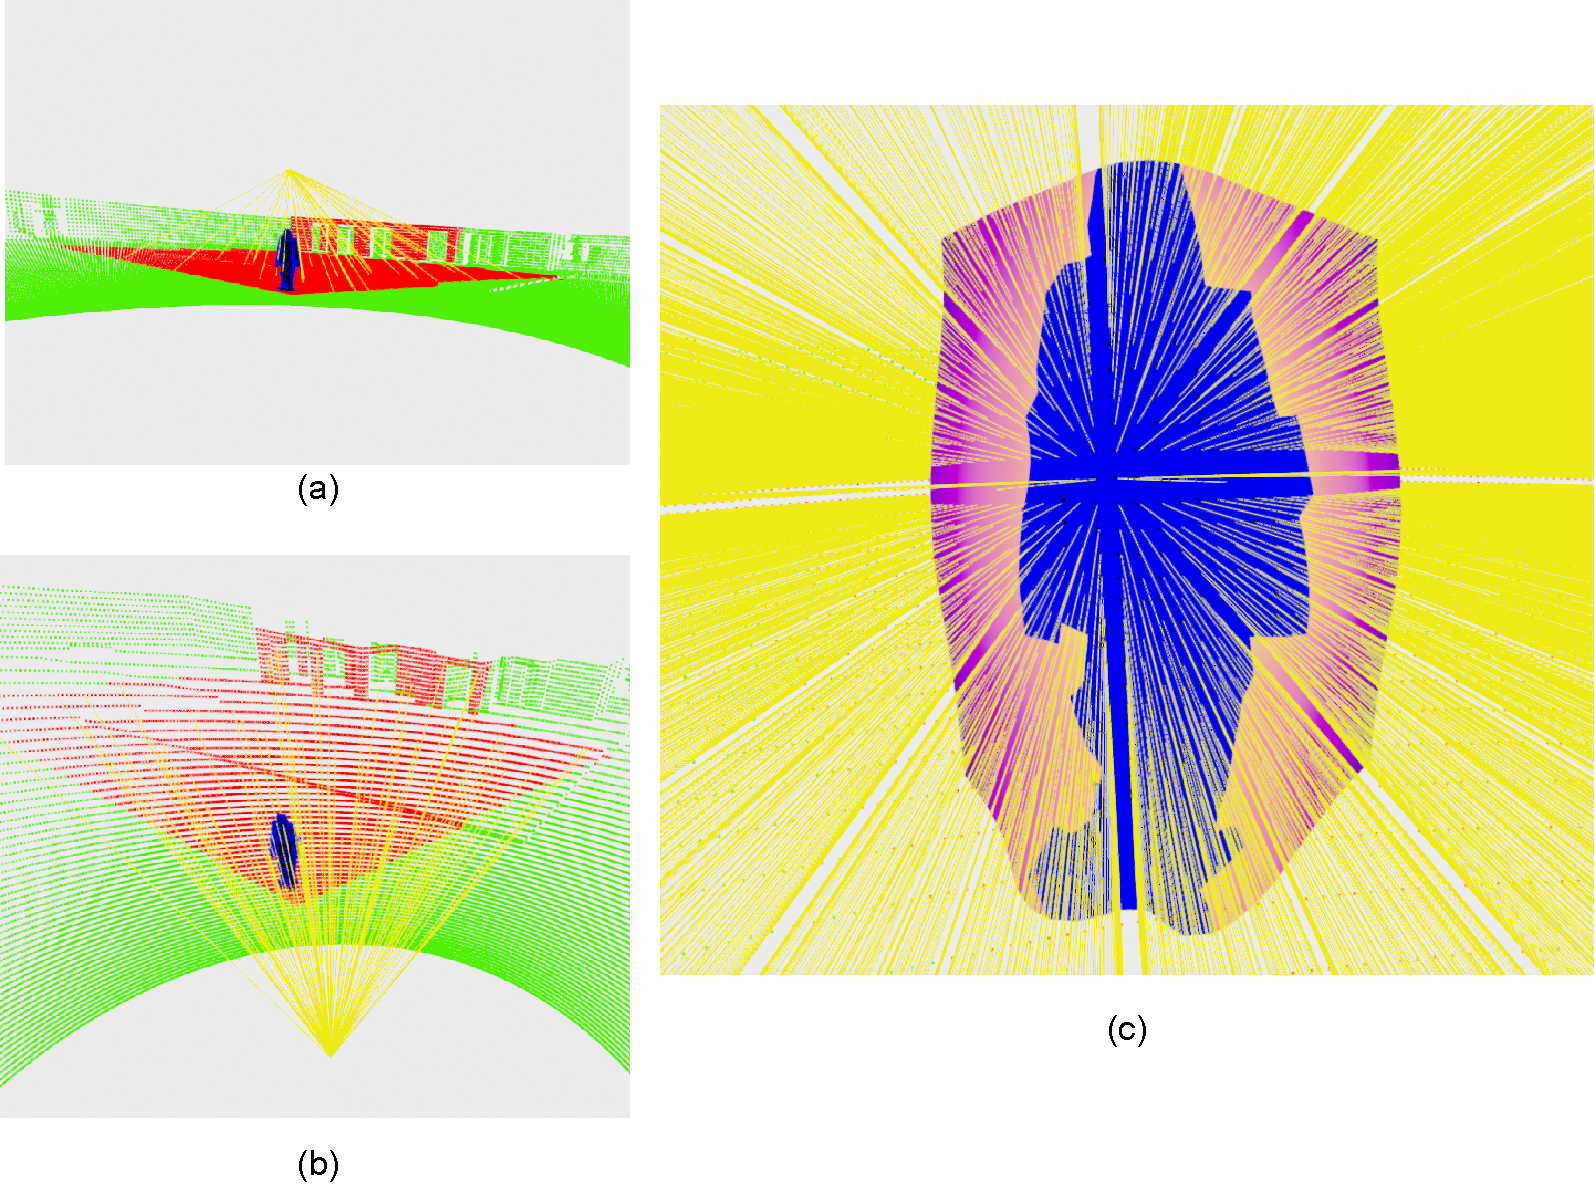
\includegraphics[width=1\linewidth]{97_graphics/results/raycasting_from_origin.pdf}
    \caption[Raycasting from Origin to the target \acrshort{roi} on the Target Scene Point Cloud (\acrshort{pcd}).]{Raycasting from Origin to the target \acrshort{roi} on the Target Scene Point Cloud (\acrshort{pcd}). (a) and (b) shows raycasting with a lower ray count. (c) shows rays intersect with the surface of the Prototype.}
    \label{fig:result-raycasting_from_origin}
\end{figure}

In the figure \ref{fig:result-raycasting_from_origin}, the yellow color lines mimic the laser rays from the LiDAR sensor. The blue color represents the surface mesh of the prototype after filtering. When the ray traverses from the origin to the target region of interest (\acrshort{roi}), it intersects the surface mesh. An example illustrating the triangle mesh and rays traversal is shown in figure \ref{fig:result-raycasting_with_triangles}.

\begin{figure}[htbp]
    \centering
    \begin{minipage}[b]{0.8\textwidth}
    \centering
    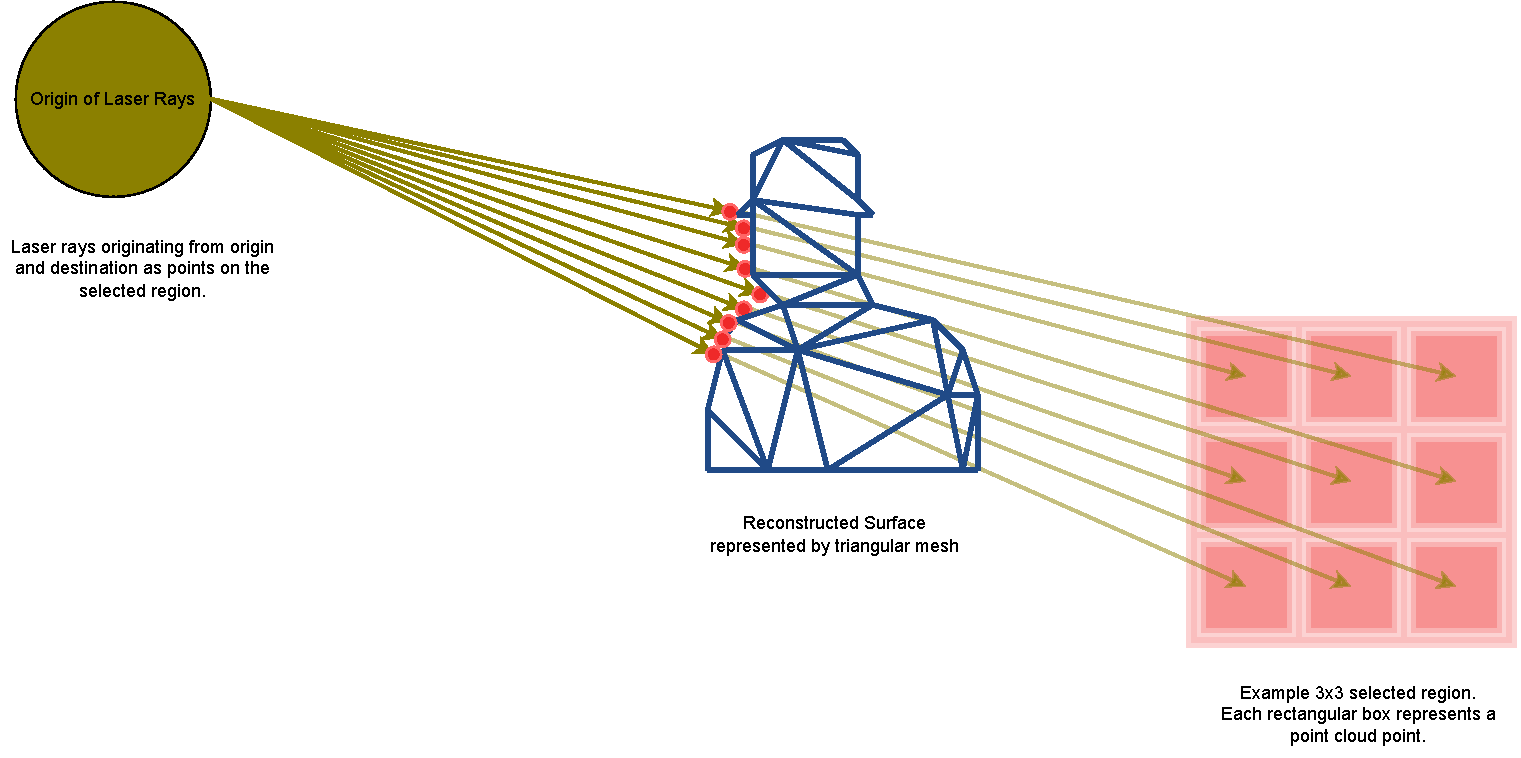
\includegraphics[width=1\linewidth]{97_graphics/results/raycasting_with_trianglesmeshes.pdf}
    \caption{Rays casting towards Prototype surface represented by a group of triangles in the triangle mesh.}
    \label{fig:result-raycasting_with_triangles}
    \end{minipage}
\end{figure}

Figure \ref{fig:result-raycasting_with_triangles} gives an example of a prototype surface represented by a group of triangles of a triangle mesh. Triangle intersected by the rays are calculated by casting rays as shown in figure \ref{fig:result-raycasting_from_origin}  and figure  \ref{fig:result-raycasting_with_triangles}. From the intersected triangles, new points of the prototype are calculated. 

\begin{figure}[htbp]
    \centering
    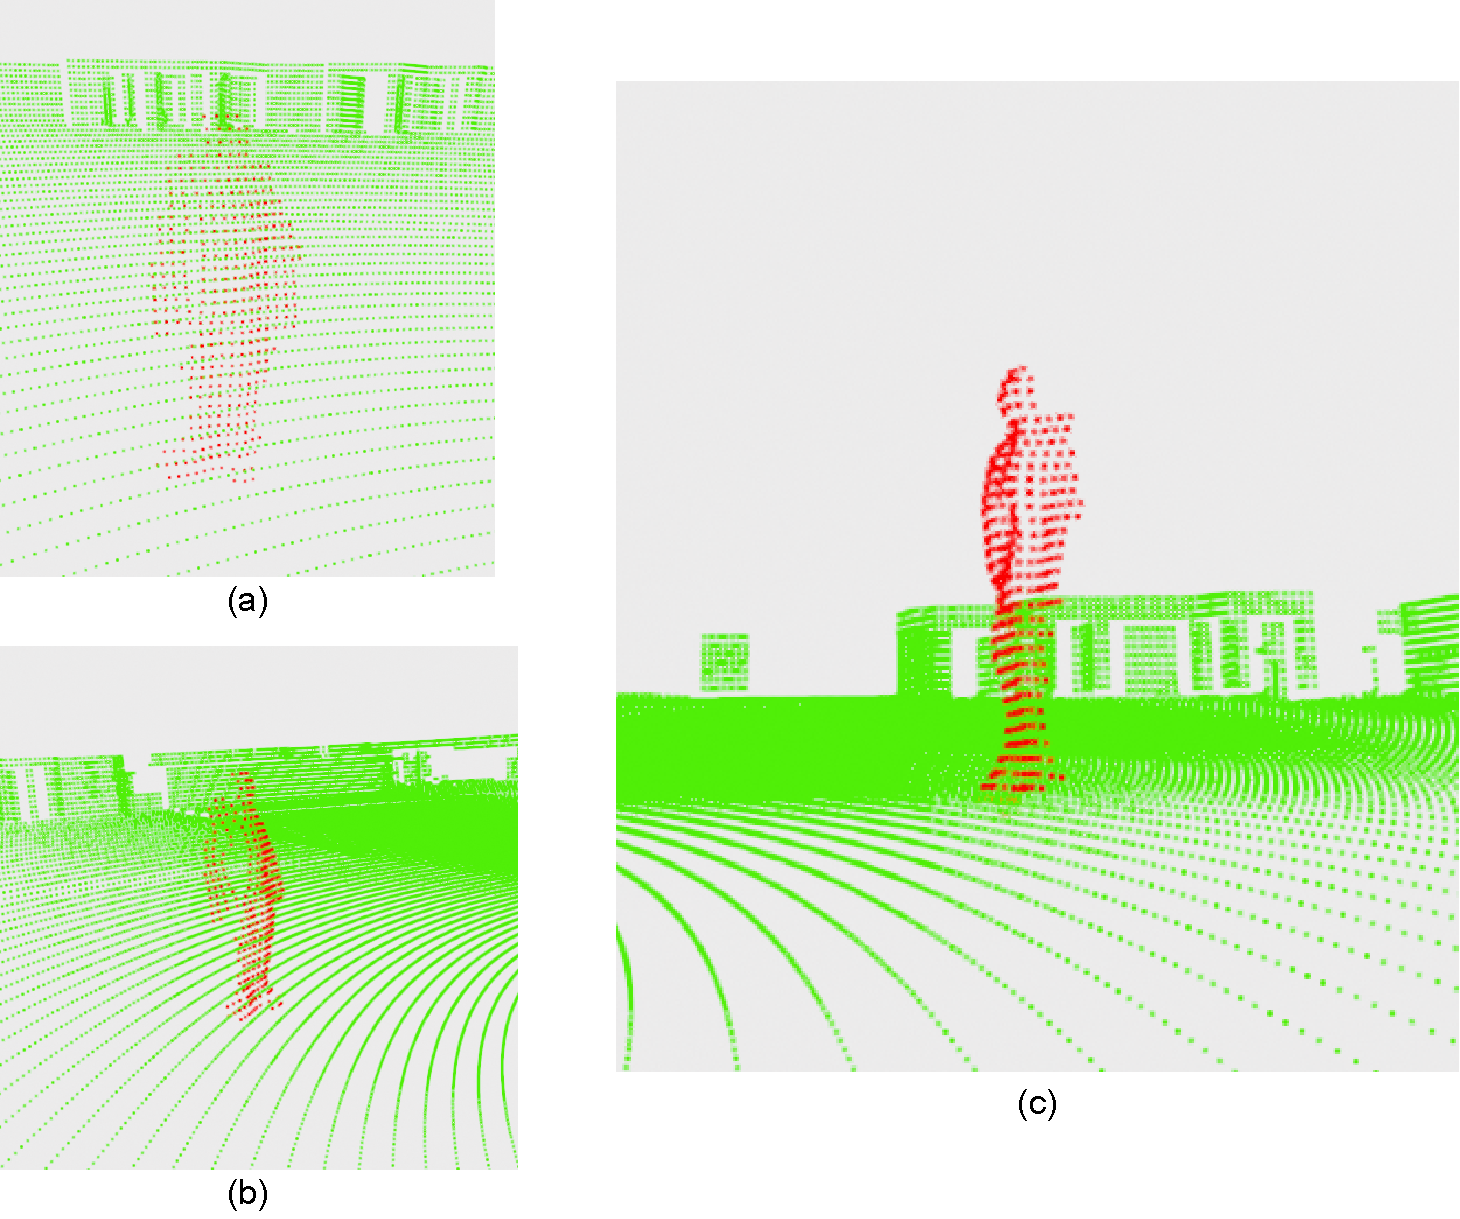
\includegraphics[width=0.6\linewidth]{97_graphics/results/raycasted_prototype.pdf}
    \caption{Raycasted Prototype visualized by red colored point cloud on the target scene cloud from different viewpoints.}
    \label{fig:result-raycasted_prototype}
\end{figure}

The raycasted point cloud of the prototype is calculated by using the equation \ref{eq:find_xyz} as shown in figure \ref{fig:concept-raycasting_single_triangle_by_t_hit}. As a final result, a point cloud of the prototype is created. We call the point cloud received after raycasting a raycasted prototype point cloud. Figure \ref{fig:result-raycasted_prototype} shows the raycasted point cloud of the prototype calculated after the raycasting method.
The red points point cloud represents the raycasted prototype in figure \ref{fig:result-raycasted_prototype}. It can be observed that the calculated point cloud of the surface mimics the surface of the original prototype (person). The raycasted prototype lies on the target scene \acrshort{pcd}. Shadow projection by the raycasted prototype on the target scene \acrshort{pcd} needs to be calculated. This is done in the next section.

\section{Shadow Casting on Target Scene by Raycasted Prototype Point Cloud}
The input to this step is a raycasted prototype point cloud on a target location (\acrshort{roi}) of the target scene \acrshort{pcd}. An experiment was done with the hidden point removal algorithm. Important parameters for the HPR algorithm are the viewpoint and the radius of the sphere for spherical flipping. Visibility of the points is determined by looking from the viewpoint of the target scene cloud. The viewpoint is set to the origin so that the process mimics the shadow projection process when a LiDAR sensor is placed at the origin. Appropriate parameters for the HPR algorithm need to be chosen to increase the shadow projection accuracy. As shown in figure \ref{fig:concept-shadow_casting_difference}, instead of using the HPR algorithm, the raycasted method is a more accurate approach for shadowcasting in our experiment. 

\begin{figure}[htbp]
    \centering
    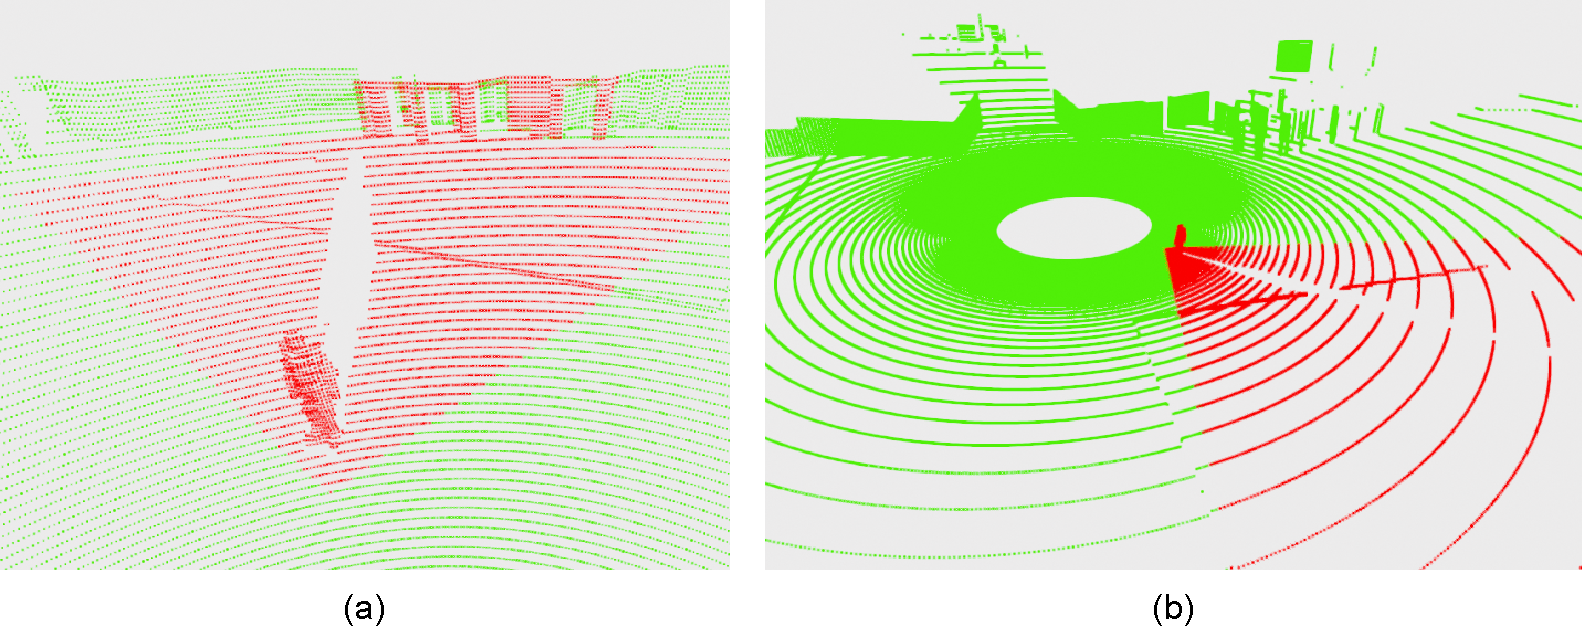
\includegraphics[width=1\linewidth]{97_graphics/results/shadow_casting_by_prototype.pdf}
    \caption{Shadow Casting by the Prototype on the Target Scene \acrfull{pcd}. (a) and (b) shows projected shadow from different viewpoints.}
    \label{fig:result-shadow_casting_by_prototype}
\end{figure}

Using the raycasted method as explained in figure \ref{fig:concept-shadow_casting_by_raycast_method}, the shadow projected by the prototype surface in the target region of the target scene cloud is calculated. The result of shadow casting is shown in figure \ref{fig:result-shadow_casting_by_prototype}. Points lying on the shadow region of the prototype are removed. Shadow was calculated for \acrshort{roi} to make the computation faster (shown by red colored region in figure \ref{fig:result-shadow_casting_by_prototype}).
			\chapter{Evaluation of the concept}
In this thesis, the evaluation of the project output is conducted with a focus on validating the accuracy of the obtained results, rather than demonstrating improvements over existing \acrshort{sota} 3D object detection models.
To evaluate the results obtained from the study, a two-step analysis is conducted. Firstly, the raycasted point cloud is analyzed, followed by an examination of the casted shadow.

\begin{figure}[htb]
    \centering
    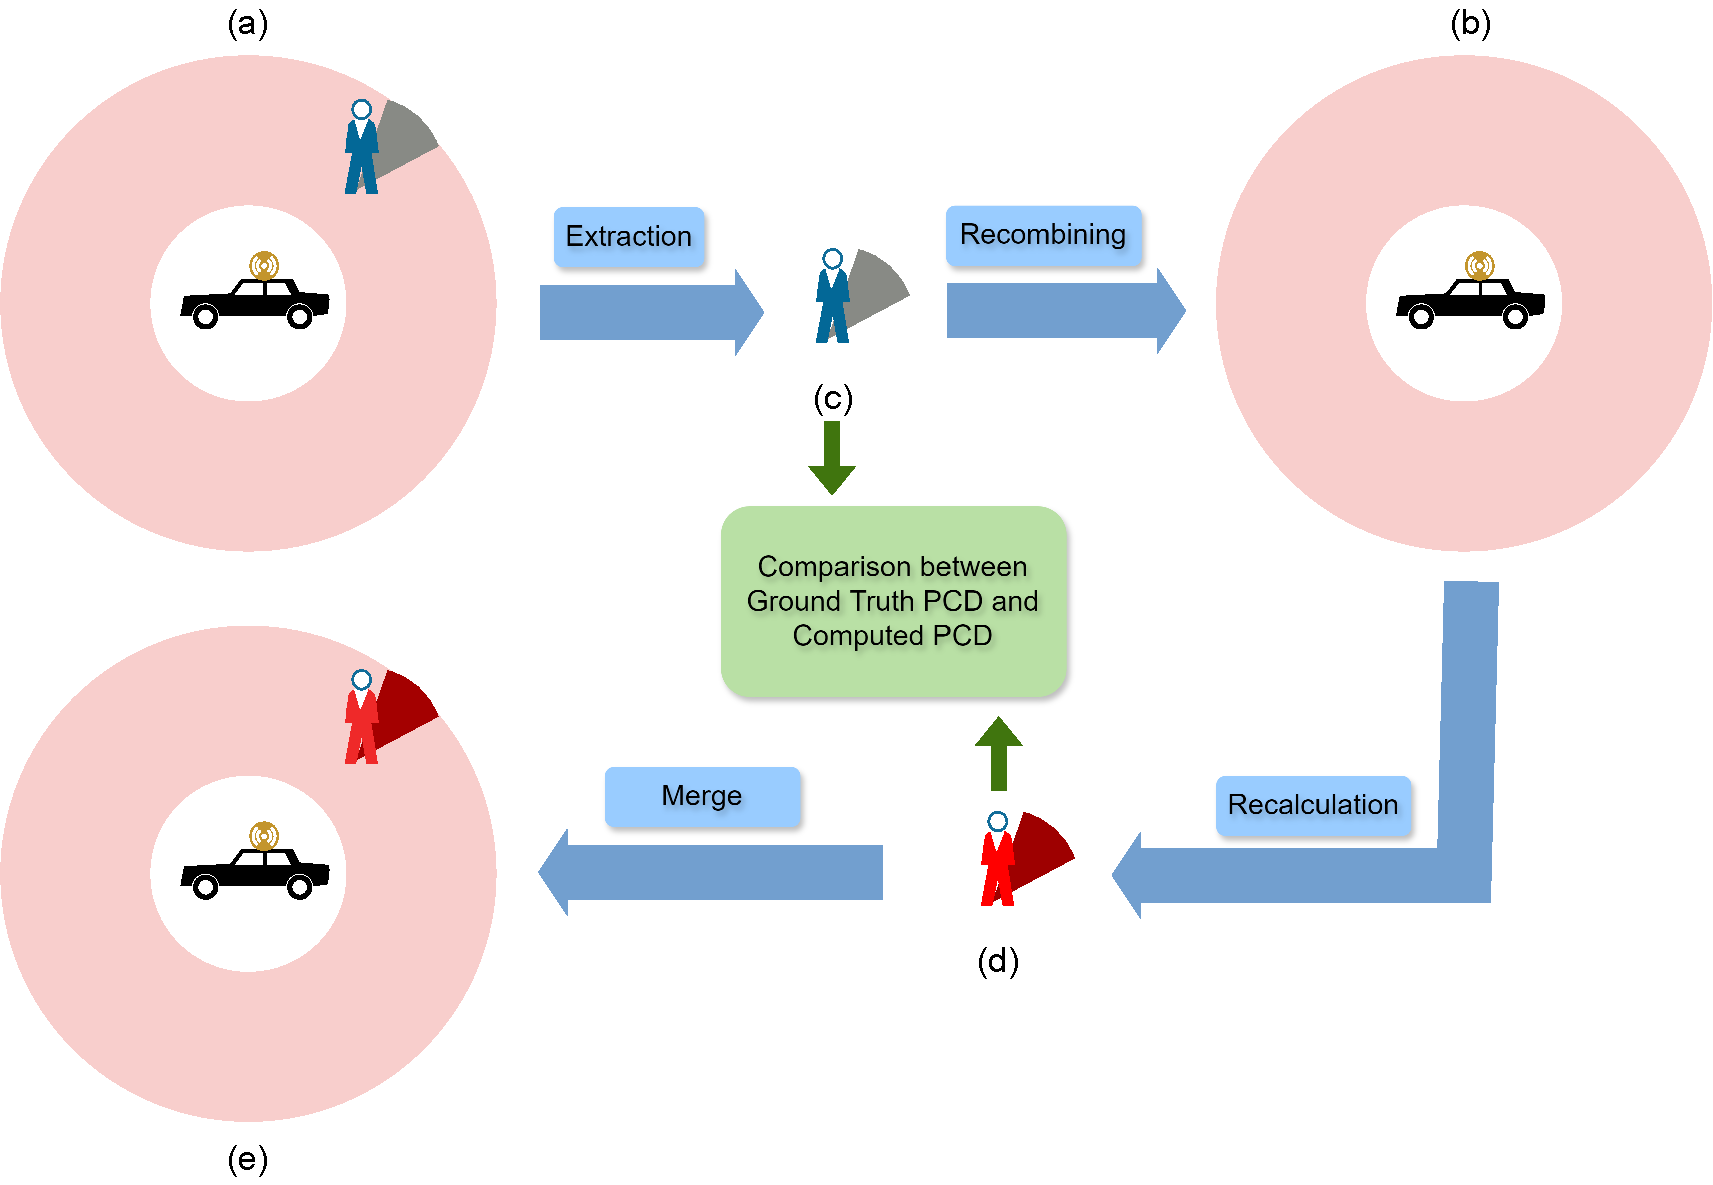
\includegraphics[width=0.75\linewidth]{97_graphics//evaluation/evaluation_step_diagram.pdf}
    \caption[Evaluation Concept Diagram.]{Evaluation Concept Diagram. (a) and (b) present two distinct point clouds featuring equivalent background contexts, with the sole disparity being the presence or absence of a person subject and its cast shadow. (c) showcases the isolated point cloud representing the person subject and the ground truth shadow. (d) displays the computed point cloud of the person along with its newly projected shadow onto the target scene (b). (e) Augmented target scene point cloud.} 
    \label{fig:evaluation-evaluation_step_diagram}
\end{figure}

 The assessment of the thesis output involves a comparative analysis between the point clouds represented in figure \ref{fig:evaluation-evaluation_step_diagram} \((c)\) and \ref{fig:evaluation-evaluation_step_diagram} \((d)\). Figure \ref{fig:evaluation-evaluation_step_diagram} \((c)\) represents the ground truth point cloud of the prototype (person or original prototype) and the shadow projected by the prototype. It is obtained by extracting the desired ground truth point clouds from the source scene cloud \((a)\). \((d)\) represents the prototype point cloud generated through raycasting (raycasted point cloud of prototype), accompanied by the shadow projected by this new prototype point cloud on the target scene \((b)\). This output encapsulates the culmination of the thesis work.
\((e)\) represents the final augmented target scene point cloud. The source scene point cloud \((a)\) and the target scene cloud \((b)\) are acquired from \acrshort{carla}.

\begin{figure}[htbp]
    \centering
    \includegraphics[width=0.75\linewidth]{97_graphics//evaluation/evaluation_block_diagram.pdf}
    \caption{Evaluation Overview}
    \label{fig:evaluation-evaluation_block_diagram}
\end{figure}

As outlined in figure \ref{fig:evaluation-evaluation_block_diagram}, raycasted point cloud is analyzed through four graphical representations. A scatter plot is generated wherein the distance of the prototype is varied within the target scene cloud from the origin, and subsequently, the raycasted point cloud is calculated. This analysis demonstrates a correlation between the number of raycasted points on the prototype surface and their proximity to the origin, indicating a decrease in the number of points as the distance from the origin increases. Additionally, a 3D plot comparing the original prototype and the raycasted prototype point cloud is constructed without transforming the prototype location, facilitating visual differentiation between the two sets of points in cartesian coordinate system. This is represented visually as a comparison between the point cloud of the prototype (person) represented in figure \ref{fig:evaluation-evaluation_step_diagram} \((c)\) and \ref{fig:evaluation-evaluation_step_diagram} \((d)\). Consistency between the original and raycasted prototype point clouds is affirmed by overlapping points observed in the 3D plot. Furthermore, a graph plotting the distance between corresponding points in the original and raycasted prototype clouds illustrates minimal distance discrepancies between equivalent points. Geometric feature distribution analysis, conducted using equivalent parameters, further confirms the similarity in local geometric features of points between the original prototype point cloud and the raycasted prototype point cloud.


To assess the precision of the predicted shadow, two distinct point clouds are captured: one containing a person and their casted shadow (referred to as the source scene cloud, represented by figure \ref{fig:evaluation-evaluation_step_diagram} \((a)\)), and another identical point cloud lacking the person or their shadow but maintaining similar background information (termed the target scene cloud, represented by figure \ref{fig:evaluation-evaluation_step_diagram} \((b)\)). A prototype (person) point cloud is extracted from the source scene cloud and seamlessly inserted into the target scene cloud without any transformation. Subsequently, the shadow cast by the prototype on the target scene cloud is computed. This is visually depicted as a comparison between the ground truth shadow (the shadow projected by the prototype as shown in figure \ref{fig:evaluation-evaluation_step_diagram} \((c)\) ) and the predicted shadow (the computed shadow of the raycasted prototype as shown in figure \ref{fig:evaluation-evaluation_step_diagram} \((d)\)).

The correctness of the predicted shadow is observed by plotting the confusion matrix and by computing the \acrshort{iou} score as outlined in figure \ref{fig:evaluation-evaluation_block_diagram}. A confusion matrix is constructed, wherein equivalent points between the two point clouds are identified within a \acrfull{roi} using nearest neighbor search. The confusion matrix reveals a high degree of similarity between corresponding points in the selected ROI of both point clouds. Additionally, a plot demonstrating the distance between points in the \acrshort{roi} of the predicted shadow cloud and their equivalents in the original shadow cloud further validates the accuracy of the confusion matrix. \acrfull{iou} between the predicted shadow and the ground truth shadow region is calculated, confirming the precise prediction of the shadow cast by the prototype. The discrepancy in the area of the predicted shadow compared to the ground truth shadow is attributed to the larger surface area of the reconstructed prototype (person) relative to the actual prototype.



\section{Evaluation of Raycasted Pointcloud}
A raycasted point cloud is generated by projecting rays from the origin to the surface of the prototype. The prototype surface is obtained through surface reconstruction into a triangular mesh. Methods like calculation of average distance, comparing the number of points, and comparing the vanilla 3D points were used for the evaluation of raycasted point cloud. These methods are discussed below.
\subsection{Average distance from the origin vs number of points}
With this step, we check the variation of the number of points in the raycasted point cloud when changing the position of the prototype before raycasting concerning origin. The distance between the prototype cloud and the origin of the target scene point cloud was changed by transforming the extracted prototype to a different location on the target cloud. The distance from a prototype to the origin is calculated by calculating the Euclidean distance from the origin to each point in the prototype. The average was obtained after dividing the sum of the distances of each point in the prototype by the number of points. Rays were cast to the surface of the prototype after surface reconstruction.  Change in points number based on different locations of the transformed prototype on the target scene cloud is observed.

\begin{figure}[htbp]
    \centering
    \includegraphics[width=0.8\linewidth]{97_graphics/evaluation/avg_distn_vs_points_numbers.pdf}
    \caption{Averge distance from the origin [in meters] vs Number of points in Raycasted Point cloud}
    \label{fig:evalution_avg_distn_vs_points_number}
\end{figure}
In this figure \ref{fig:evalution_avg_distn_vs_points_number}, the original prototype is positioned at about 7 meters from the origin. The prototype was moved closer toward the origin and farther away from the origin on the target cloud, and the raycasted point cloud of the prototype was calculated. From the graph, as shown in figure \ref{fig:evalution_avg_distn_vs_points_number}, it can be seen that the number of points on the raycasted prototype decreases after an increase in the average distance between the prototype and the origin (more than 7 meters distance). The number of points of the raycasted prototype increases when the prototype is transformed closer to the origin (less than 7 meters distance).

\subsection{3D plot of the original and raycasted prototype}\label{sec:3dplot}
To visualize the similarities between the corresponding points on the original and raycasted prototype point cloud, a simple 3D plot in the XYZ axis can be analyzed. For this evaluation, the difference between the original prototype and the raycasted prototype is shown where the raycasting was done without transforming the position of the prototype on the target cloud.

\begin{figure}[htbp]
    \centering
    \includegraphics[width=0.75\linewidth]{97_graphics//evaluation/original_vs_raycasted_pcd.pdf}
    \caption[Visualization of point clouds]{Visualization of point clouds (a) Original prototype point cloud (b) Raycasted point cloud of prototype}
    \label{fig:evaluation-original_vs_raycasted_pcd}
\end{figure}

Figure \ref{fig:evaluation-original_vs_raycasted_pcd} \((a)\) shows the point cloud of the prototype (person) before raycasting (by the black color points). \((b)\) shows the point cloud of the prototype evaluated after raycasting  (by the red color points). The raycasted point cloud in figure \ref{fig:evaluation-original_vs_raycasted_pcd} \((b)\) is computed without transforming the orientation of the prototype to compare the difference in corresponding points between the two point clouds.


\begin{figure}[htbp]
    \centering
    \includegraphics[width=1\linewidth]{97_graphics/evaluation/3dxyz_plot.pdf}
    \caption{3D XYZ Plot}
    \label{fig:evaluation_3dplot}
\end{figure}

The graph can be viewed in figure \ref{fig:evaluation_3dplot}. The black points in the graph correspond to the point in the prototype before raycasting (representing the point cloud shown in figure \ref{fig:evaluation-original_vs_raycasted_pcd} \((a)\) ). The red points in the graph correspond to the point of the prototype after raycasting (representing the point cloud shown in figure \ref{fig:evaluation-original_vs_raycasted_pcd} \((b)\) ). It can be observed that most of the red points overlap the black points in space, which proves that there is a low difference between the original prototype point cloud and the prototype cloud after raycasting. Most of the red points that do not overlap with the black points are due to the bigger area of the reconstructed surface of the prototype. Proper filtering of the reconstructed surface could result in the removal of the red outliers.

\subsection{Distance between the corresponding points}
Distance between the corresponding points was calculated between the original prototype cloud and the prototype cloud after raycasting. The raycasting was performed on the original prototype surface without transformation. We calculated the average distance between the black points and the corresponding red points of figure \ref{fig:evaluation_3dplot}. To find the corresponding points between two clouds, spheres with different values of radius were experimented with for the calculation of the nearest neighbor. Neighbors for a point in the original prototype were calculated from the raycasted point cloud that falls within the radius of the sphere, centered around the ego point. The neighbor that has the minimum distance from the ego point is chosen. This point in the raycasted prototype is considered the equivalent point of the ego point in the original prototype. Sphere size can be lower or higher for neighbor search. This is because whatever the size of the sphere, we are extracting a point from the neighborhood inside the sphere that has the least distance from the ego point or center of the sphere. However, too low value for radius might lead to not finding any neighbors.
\begin{figure}[htbp]
    \centering
    \includegraphics[width=1\linewidth]{97_graphics/evaluation/distn_betn_corresponding_points_in_raycasting.pdf}
    \caption{Distance between the corresponding points in centimeters}
    \label{fig:evaluation_distn_corresponding_points}
\end{figure}

Figure \ref{fig:evaluation_distn_corresponding_points} shows plots of the distance between the black points and their equivalent red points from figure \ref{fig:evaluation_3dplot}. Figure (a) is plotted after finding the nearest neighbor with a search within the sphere of radius 3 cm centered around an ego point. When searching the neighbor with a sphere of radius 3cm, out of 408 points in the raycasted point cloud, 163 number of equivalent points were not found in the original point cloud. Using a higher radius value for neighbor search (20 cm), all the points in the red points were found to have their equivalent black points. This is shown by part (b) of the figure. The figure shows that a high concentration of equivalent points is situated within 0-3 cm distance apart from eachother.

\subsection{Surface Variation Plot}
Surface variation for the point cloud represented by red points and black points in figure \ref{fig:evaluation_3dplot} was calculated and plotted.

\begin{figure}[htbp]
    \centering
    \includegraphics[width=1\linewidth]{97_graphics/evaluation/sv_plots.pdf}
    \caption{Surface Variation plot}
    \label{fig:evaluation-sv_plots}
\end{figure}

For this experiment, a radius of 30cm with a maximum value of the nearest neighbor was taken to be 6 as a parameter to calculate the nearest neighbor using KDTree. Using the formula for surface variation as described in equation \ref{eq:surf_var}, surface variation for each point in the point cloud is calculated. The obtained result is normalized on a scale of 0 to 1 and the corresponding plot is displayed as shown in figure \ref{fig:evaluation-sv_plots}. The figure shows the similarities in geometric features (surface variation )between the two point clouds.


\section{Evaluation of Casted Shadow}
For the evaluation purpose, point cloud representing a "flat" surface was captured from the \acrshort{carla}. This point cloud represents a target scene where we would like to do a shadow casting. A prototype "person" was spawned in some location in the target region without changing the orientation of the lidar sensor and the point cloud was saved. This point cloud corresponds to the source scene cloud. The prototype cloud is extracted from the source scene cloud and placed in the target scene cloud. Shadow casting by the prototype is performed on the target cloud and the final point cloud is saved. The prototype person is not transformed in the target scene. The difference between the target scene cloud and the source scene cloud is the availability of the person and its casted shadow, the rest of the points are similar in both point clouds, i.e. background information is similar on both point clouds. A region is selected from the source scene cloud which constitutes of shadow projected by the prototype. This region is the ground truth shadow region as shown in figure \ref{fig:evaluation-shadow_difference_roi} \((a)\). The corresponding region is selected on the target scene cloud where the raycasted point cloud of the prototype is computed and the shadow projected by the new prototype point cloud is calculated. This region is the predicted shadow region as shown in figure \ref{fig:evaluation-shadow_difference_roi} \((b)\).
\begin{figure}[htbp]
    \centering
    \includegraphics[width=1\linewidth]{97_graphics//evaluation/shadow_difference_roi.pdf}
    \caption[Shadow casted by the prototype]{Shadow casted by the prototype (person) on a ROI, represented by green color region(a) Ground truth shadow (b) Predicted shadow}
    \label{fig:evaluation-shadow_difference_roi}
\end{figure}

Figure \ref{fig:evaluation-shadow_difference_roi} shows the shadow projected by the prototype. The green-colored region on both \((a)\) and \((b)\) represents the approximate shadow projected by the prototype. \((a)\) represents ground truth shadow region and \((b)\) represents predicted shadow region.  Shadow is calculated and computed for only a selected region on the target scene cloud. The selected \acrfull{roi} is shown by the red color point in figure \ref{fig:evaluation-shadow_difference_roi}.

\subsection{Confusion Matrix}
Comparison between the shadow is done by finding the corresponding points between the ground truth shadow and the anticipated shadow, i.e. between points in figure \ref{fig:evaluation-shadow_difference_roi} \((a)\) and \((b)\). The nearest neighbor search was done to find the equivalent points in the selected ROI of the ground truth shadow and anticipated shadow cloud. The radius of the sphere for the neighbor search was taken to be 3 centimeters. If no neighbors were found on the corresponding point cloud within this region, the point was considered to be not found. From the found neighbors, based on some threshold value, the neighbors were filtered. If there exists a neighbor after filtering with some threshold distance, the point was considered to be found on both point clouds. If not, the point was labeled as not found. A confusion matrix is plotted as shown in figure \ref{fig:evaluation_cm}.


\begin{figure}[htbp]
    \centering
    \includegraphics[width=1\linewidth]{97_graphics/evaluation/cm_shadowcast.pdf}
    \caption{Confusion matrix}
    \label{fig:evaluation_cm}
\end{figure}

Some observations can be made from the confusion matrix in figure \ref{fig:evaluation_cm}. Equivalent points for 150 points from the ground truth shadow were not found in the predicted shadow. 2 points available on the predicted shadow cloud were not found in the ground truth shadow cloud. 4032 corresponding points were found in both regions. Unable to say about the points not found on both, the true negative section in the confusion matrix is labeled as 0. From the confusion matrix, the following metrics are observed. 
\begin{itemize}
    \item \textbf{True Positive : }4032
    \item \textbf{True Negative : }0
    \item \textbf{False Positive : }2
    \item \textbf{False Negative : }150
    \item \textbf{Accuracy : }0.963
    \item \textbf{Precision : }0.999
    \item \textbf{Recall : }0.964
    \item \textbf{F1-Score : }0.981
\end{itemize}


% Using the formula for the metrics calculation, table \ref{tab:cm_metrics} is constructed.
% \begin{table}
%     \centering
%     \resizebox{0.2\textwidth}{!}{%
%     \begin{tabular}{|c|c|}
%         \hline
%         \textbf{Metric} & \textbf{Value} \\ \hline
%          Accuracy & 0.963 \\ \hline
%          Precision & 0.999 \\ \hline
%          Recall & 0.964 \\ \hline
%          F1-Score & 0.981 \\ \hline
%     \end{tabular}%
%     }
%     \caption{Performance metrics from the confusion matrix plot of figure \ref{fig:evaluation_cm}}
%     \label{tab:cm_metrics}
% \end{table}

The calculation proves that the shadow projection has a high accuracy and a very low error rate. 

Figure \ref{fig:evaluation-distn_betn_corresponding_points_in_shadowcasting} shows the distance between the corresponding points in the predicted shadow cloud and the ground truth shadow cloud. The figure verifies that the points that were considered to be similar in both regions are very similar as the distance between the similar points is in the order of \(1e-9\).

\begin{figure}[htbp]
    \centering
    \includegraphics[width=1\linewidth]{97_graphics//evaluation/distn_betn_corresponding_points_in_shadowcasting.pdf}
    \caption{Distance between corresponding points in Shadowcasting}
    \label{fig:evaluation-distn_betn_corresponding_points_in_shadowcasting}
\end{figure}

\subsection{Intersection over Union}
For the calculation of \acrfull{iou}, the contour points of the shadow region were first extracted for both the point clouds(ground truth shadow and predicted shadow region). The contour points are represented by the boundary points of the green-colored region of figure \ref{fig:evaluation-shadow_difference_roi}. The extracted 3d-points were projected to the XY plane; i.e. by making the z-value of each point zero. The area of the region occupied by the surface bounding the contour points (i.e. the shadow region) was calculated. This is shown approximately by green-colored region in figure \ref{fig:evaluation-shadow_difference_roi}. The absolute region representing the ground truth shadow and predicted shadow is shown in figure \ref{fig:evaluation-shadow_gt_pred}.
\begin{figure}[htbp]
    \centering
    \includegraphics[width=1\linewidth]{97_graphics//evaluation/shadow_gt_pred.pdf}
    \caption{Plot of Ground truth shadow and Predicted Shadow}
    \label{fig:evaluation-shadow_gt_pred}
\end{figure}

Figure \ref{fig:evaluation-shadow_iou} (a) shows the intersection region between the ground truth shadow and predicted shadow by green color. (b) shows the union area between the two regions. Some observations can be made as below. All the observation units (except IoU) are \((m^2)\).
\begin{itemize}
    \item \textbf{Area of Ground Truth Shadow : }17.318
    \item \textbf{Area of Predicted Shadow : }25.886
    \item \textbf{Area of Intersection : }17.293
    \item \textbf{Area of Union : }25.910
    \item \textbf{IOU : }0.667
    \item \textbf{Area in Ground truth shadow not in Predicted shadow : }0.0248
    \item \textbf{Area in Predicted shadow not in Ground truth shadow : }8.592
    \item \textbf{Percentage of Ground truth shadow accurately predicted :} $\frac{17.318 - 0.0248}{17.318}$ \( = 99.856\%\) 
\end{itemize}


% \begin{table}
%     \centering
%     \resizebox{0.8\textwidth}{!}{%
%     \begin{tabular}{|c|c|}
%         \hline
%         \textbf{Metric} & \textbf{Area \((m^2)\)} \\ \hline
%          Ground Truth Shadow & 17.318 \\ \hline
%          Predicted Shadow & 25.886 \\ \hline
%          Area of Intersection between ground truth and predicted shadow & 17.293 \\ \hline
%          Area of Union between ground truth and predicted shadow & 25.910 \\ \hline
%          Area in ground truth shadow not in predicted shadow & 25.910 \\ \hline 
%          Area in predicted shadow not in predicted shadow & 25.910 \\ \hline 
%     \end{tabular}%
%     }
%     \caption{Performance metrics from the confusion matrix plot of figure \ref{fig:evaluation_cm}}
%     \label{tab:cm_metrics}
% \end{table}

\begin{figure}[htbp]
    \centering
    \includegraphics[width=1\linewidth]{97_graphics//evaluation/shadow_iou.pdf}
    \caption{Intersection and Union between the ground truth shadow region and predicted shadow region plot}
    \label{fig:evaluation-shadow_iou}
\end{figure}

It can be observed from the findings about the accuracy of ground truth shadow. About \(99.856 \%\) of the ground truth shadow region was predicted. The IoU score was 0.667. It can be improved by filtering the reconstructed surface to accurately represent the prototype.


			%\input{03_texfiles/Kapitel_Projektmanagement}
			\chapter{Discussion and Conclusion}
Novel point cloud scenarios within the context of \acrfull{had} systems were generated by injecting a \acrfull{pcd} object from a source scene \acrshort{pcd} into a target scene \acrshort{pcd}. By using the orientation of the prototype in the source scene \acrshort{pcd}, the prototype was transformed into a target location on the target point cloud. After the transformation, a new point cloud for the transformed prototype was calculated and the shadow casted by the newly computed prototype \acrshort{pcd} on the target scene \acrshort{pcd} was observed.

\section{Challenges}

The initial phase of experimental data collection from CARLA posed hurdles due to the necessity of meeting system requirements for running CARLA and ensuring compatibility with all requisite versions of dependent software such as ROS2, carla-ros-brige, and the operating system. Placing the extracted prototype point cloud data (PCD) into a designated target location also presented difficulties. Initial attempts using the \acrfull{icp} registration algorithm proved ineffective, particularly in areas with sparse points in the point cloud. Instead, successful placement of the extracted prototype \acrshort{pcd} was achieved by transforming it based on the centroid of the filtered ground plane. To address the challenge of unknown surfaces of a prototype that are not visible to the LiDAR sensor, the extracted prototype point cloud is rotated during transformation within the target scene PCD. This rotation is determined by utilizing the centroid of the prototype both before and after translation. Additionally, obtaining a realistic point cloud of the prototype that accurately replicated the real LiDAR beam scan patterns at various positions within the target scene \acrfull{roi} posed a challenge. This was addressed by leveraging the points within the target point cloud to simulate the laser beams for raycasting, thereby generating a realistic LiDAR point cloud of the prototype at a desired \acrshort{roi} without requiring knowledge of the LiDAR configuration. Furthermore, accurately calculating the realistic shadow projected by the prototype onto the target ROI of the scene cloud initially proved to be error-prone when using the \acrfull{hpr} algorithm. However, the process was refined by tracking casted rays to the target ROI, facilitating the computation of a realistic shadow projected by the prototype onto the ROI of target scene \acrshort{pcd}.



\section{Future Works}
The project could be improved in various ways.
\begin{itemize}
    \item Extraction of the prototype \acrshort{pcd} from the source scene \acrshort{pcd} is done by using surface variation only. Several other geometric features could be used to remove the false positives. This is required in the case when working with real-world LiDAR data.
    \item Experiment is done for the extraction of the pedestrian point cloud. Methods need to be tested for various objects such as cars, bikes, etc.
    \item By scanning an object from a different angle view and by the point cloud registrations technique, a point cloud representing a complete hollow 3D object could be constructed. Such objects could be rotated in any way in the target location. This results in an increase in the variability of scenarios.
    \item The centroid of points from the remaining points in the \acrshort{roi} on the source scene \acrshort{pcd} is calculated after cropping the prototype \acrshort{pcd}, which is later used in the transformation of the prototype on the target scene \acrshort{pcd}. If the remaining points after filtering the prototype \acrshort{pcd} consist of points from the prototype or higher z-values than the ground plane, then the transformation would be wrong. Eg. the transformed prototype point cloud lies 1 meter above the target ground plane i.e. levitating in the air.
    \item Experiment is done on flat surfaces point cloud. Improvements could be made in the future by adding support for non-planar surfaces.
    \item The required placement of objects needed for scenario-based testing should be properly analyzed.
    \item The Prototype \acrshort{pcd} could only be extracted if it is standing on the ground plane point cloud. There could be a scenario where a prototype could be very near to the LiDAR sensor where there is no ground plane \acrshort{pcd}. Because of the field of view of the LiDAR sensor, only the upper region of prototype surface is scanned by the LiDAR scanner. The ground plane where the prototype is situated or the lower region of prototype points is not visible. Current method needs to be updated for extracting such objects as there is no ground plane point cloud to calculate a reference centroid for transformation.
    \item The Raycasting process depends on the original direction of the laser on the target scene \acrshort{pcd}. If the points represented on the target scene \acrshort{pcd} are erroneous, then the resulting raycasted points will be erroneous.
    \item Accurately representing the surface of the prototype \acrshort{pcd} after surface reconstruction would result in a reduced error during raycasting and shadowcasting.
    \item To replicate the behavior of LiDAR sensors in real-world settings, random dropout, and noise can be introduced.
    \item At present, the intensity of points can be determined by assigning an intensity function to points according to how far they are from the LiDAR source. However, there is a need to develop methodologies that take into account and preserve the reflective characteristics of the prototype surface.
    \item Currently, manual selection of a region is done for the insertion of the extracted prototype in a desired region of the target scene \acrshort{pcd}. Finding an appropriate region automatically for the insertion of the prototype on the target region of the target scene \acrshort{pcd} could remove the step for manual intervention. If the manual selection of the \acrshort{roi} step is eliminated then by using the pre-saved extracted prototype \acrshort{pcd}, real-time injection on the target scene \acrshort{pcd} could be possible.
    \item In this thesis, the challenge of class imbalance is addressed by leveraging the reuse of existing scenes. However, it is imperative to further investigate methods that accommodate scenarios without the reuse of pre-existing scenes.
\end{itemize}

\section{Conclusion}
Thus, novel scenario-driven test data, in the context of \acrfull{had} Systems, were synthesized through LiDAR data augmentation. This involved extracting a prototype point cloud utilizing the geometric features of 3D points in the local neighborhood of the point cloud. The prototype surface was then reconstructed at a designated location within the target scene \acrshort{pcd}, and new point clouds for the prototype were calculated based on the original direction of laser rays in the target scene \acrshort{pcd}. Subsequently, shadows projected by the newly computed prototype \acrshort{pcd} onto the target scene \acrshort{pcd} were determined. Thus, resulting in the creation of a new point cloud representing the altered scene. Evaluation of the approach was conducted by analyzing two point clouds representing identical backgrounds: one with a ground truth prototype (foreground object) and another without. This methodology allowed for the examination of discrepancies between the ground truth and the calculated new point cloud without the necessity of considering differing background point clouds. 
\parencite{padusinski2024machine} explains the necessity of interpreting objects at different levels of granularity grades. Using the reconstructed surface to calculate the point cloud of the object gives a raycasted point cloud with some discrepancies due to varying surface area. Most importantly, the intensities of the original \acrshort{pcd} are not taken into account in the raycasted \acrshort{pcd} as the surface reconstruction step removes that information by creating a \acrshort{cad} model from extracted prototype \acrshort{pcd}. In case of the recombining of the extracted prototype \acrshort{pcd} to the target scene \acrshort{pcd} without transformation, the extracted prototype \acrshort{pcd} can be merged with the target scene \acrshort{pcd} instead of the raycasted \acrshort{pcd} to save the information inherent to the original person object (such as the color of skin, t-shirt, etc.).

The study effectively tackled the challenge of class imbalance between foreground objects and background scenes within \acrfull{had} systems through an innovative strategy leveraging LiDAR data augmentation. Significantly, this was achieved without the reliance on annotated LiDAR data during prototype extraction and without prior knowledge of the LiDAR characteristics of the target dataset to be augmented. This novel process circumvents the necessity for 3D semantic models or pre-existing CAD models. Furthermore, the augmentation process demonstrated its potential to mitigate deficiencies within scenarios by seamlessly integrating foreground objects into background scenes, thereby generating diverse and novel concrete scenarios. 
The methodology investigated in this study could benefit from improvements in the surface reconstruction phase. By incorporating the automated selection of regions within the target scene, the process could facilitate real-time injection of foreground objects and the generation of extensive datasets featuring diverse scenarios, all without requiring manual intervention. Such enhancements hold promise for integration into testing phases aimed at assessing the performance of \acrfull{had} systems, thereby advancing the evaluation of system efficacy.


\printbibliography

\end{document}